\documentclass[11pt,twoside,letterpaper,twocolumn]{report}

\usepackage{fancyhdr}
\usepackage{parskip}
\usepackage{xcolor}
\usepackage{gensymb}
\usepackage[Lenny]{fncychap}
\usepackage{titlesec}
\usepackage{pifont}
\usepackage{array}
\usepackage{float}
\usepackage{enumitem}

%\usepackage{stix} % Use the STIX fonts

%\usepackage{fourier} % Utopia font

% Use EB-Garamond fonts. Doesn't play nicely with Github's PDF preview so disable for now.
%\usepackage[cmintegrals,cmbraces]{newtxmath}
%\usepackage{ebgaramond-maths}
%\usepackage[T1]{fontenc}


\usepackage[backend=biber]{biblatex}
%\usepackage{biblatex}
\addbibresource{notebook.bib}

\usepackage{xurl}
\usepackage{hyperref}
\hypersetup{
    colorlinks=true,
    linkcolor=blue,
    filecolor=magenta,
    urlcolor=cyan,
    pdftitle={CFI Notebook},
    pdfpagemode=FullScreen,
}

\usepackage{graphicx}
\graphicspath{ {./images/} }

% Dedication
% https://tex.stackexchange.com/questions/102830/dedication-page-in-article-class
%\usepackage[paper=letterpaper,left=30mm,right=30mm,top=40mm,bottom=40mm]{geometry}
\usepackage[paper=letterpaper,left=15mm,right=15mm,top=15mm,bottom=25mm]{geometry}
\newenvironment{dedication}
  {\clearpage           % we want a new page
   \thispagestyle{empty}% no header and footer
   \vspace*{\stretch{1}}% some space at the top
   \itshape             % the text is in italics
   \raggedleft          % flush to the right margin
  }
  {\par % end the paragraph
   \vspace{\stretch{3}} % space at bottom is three times that at the top
   \clearpage           % finish off the page
  }


\author{Jos\'e Hiram Soltren}
\title{CFI Notebook}
\begin{document}

%\maketitle

% https://www.latextemplates.com/template/vertical-line-title-page

\begin{titlepage} % Suppresses displaying the page number on the title page and the subsequent page counts as page 1

\raggedleft % Right align the title page
\rule{1pt}{\textheight} % Vertical line
\hspace{0.05\textwidth} % Whitespace between the vertical line and title page text
\parbox[b]{0.75\textwidth}{ % Paragraph box for holding the title page text, adjust the width to move the title page left or right on the page
{\Huge\bfseries CFI Notebook}\\[2\baselineskip] % Title
{\large\textit{Reference notes for the private, instrument, and \\ 
    commercial pilot candidate and instructor}}\\[4\baselineskip] % Subtitle or further description
{\Large\textsc{jos\'e hiram soltren}} % Author name, lower case for consistent small caps

\vspace{0.5\textheight} % Whitespace between the title block and the publisher

{\noindent Soltren Consulting LLC}\\[\baselineskip] % Publisher and logo
{\noindent \today }\\[\baselineskip] % Publisher and logo
}

\end{titlepage}

\begin{dedication}
For Zo\"e, Sebastian, and Malcolm, who hopefully find\\
as much inspiration from me as I do from them.\\
I hope they learn to fly one day too.
\end{dedication}

\section*{Introduction}

DISCLAIMER: As of this writing, the author is NOT an FAA-certified ground or flight instructor. This book must be used for reference purposes, only. For the purpose of ground or flight instruction, the reader is directed to consult a ground instructor, certificated flight instructor (CFI) or certificated flight instrument instructor (CFII).

\pagebreak
\section*{Acknowledgements}

It takes a village to keep a small airplane in the air, and to teach a pilot.

Most immediately, I must call out John Grieger and Brent Kelley, my partners (as of this writing) in our shared ownership of N36262, our 1978 Piper Lance II. With their help I have learned more about what it means to be the owner and operator of an aircraft than I could have hoped to otherwise. I appreciate Martyn Atterton for selling me his share of the airplane when he decided it was time to hang up his wings.

My thanks go to the crew of phenomenal flight instructors with whom I have had the pleasure of flying throughout my aviation career. In reverse chronological order of last flight, these are: Eric Lenk, Steve Jennings, Lawrence Spinetta, Mark Kobelin, Stephen Pitts, and Tim Stingle. Each has brought their own unique perspective of flight and instruction to the table. All have helped me to shape and refine my own instructional style. With them together, I feel like I've gotten the best combination of military flight instruction, airline flight instruction, aeronautical university instruction, and home-grown Part 61 instruction that I could have possibly gotten as a low hour pilot.

I would also like to thank the fantastic crew of safety pilots who have flown with me through the years, regardless of who was in which seat. These would be Karthik Shivashankar, Leland Freeman, David Kindley, Geoffrey Blake, Robert Curtis, David Loia, and Jeff Chern. It is somewhat refreshing to know that all pilots, regardless of their seniority, are still students and are still humans.

My co-owners in N36262 have been a resource as well. John Grieger is an accomplished pilot in his own right. Our hangar flying sessions have made us both better pilots.

Due credit goes to Joe Locasto, the old man at KSQL airport who gave me the final push to get into flying in 2011. When I lamented that flying was too expensive, he responded: ``well, it's never going to be cheaper, so what are you waiting for?"

My eternal thanks go to my wife Jane, for supporting (or at least tolerating) many late nights spent putting the airplane away. When I propose a new adventure, this wonder woman never says ``no'', only, ``how?''.




\tableofcontents

\chapter{Federal Aviation Regulations}

The Federal Aviation Regulations, or FARs, provide the regulatory framework for aircraft operations within the United States. Outside the United States, the International Civil Aviation Organization, or ICAO, is the United Nations agency that helps to provide a regulatory framework. For now, let's focus on operations inside the United States.

\section{Part 21 - Certification}

\subsection{Airworthiness Certificates}

Special Flight Permits are covered in \href{https://www.ecfr.gov/current/title-14/section-21.197}{14 CFR 21.197}. There are two reasons why we might want one:

\begin{enumerate}
\item Moving a non-airworthy aircraft. We might do this in order to make repairs, to store it, to deliver or export it, to perform production flight testing, evacuation, or customer demonstration; and
\item Ferry flights, for which we may need additional fuel tanks and weight for added range.
\end{enumerate}

The local FSDO can provide such a permit.

\section{Part 23 - Airworthiness for Normal (non Transport) Airplanes}

Airworthiness is the measure of an aircraft's suitability for safe flight. FAR parts 21 through 39 concern themselves with airworthiness. In this section, we'll touch upon a few common areas.

\subsection{Aircraft Categories}

There was a big shake up of FAR 23 in 2016. ``With respect to the number of categories on a TC, the FAA is eliminating the commuter, utility, and acrobatic airplane categories in part 23 for the reasons explained in the NPRM. Therefore, airplanes certified under new part 23 have only one category: normal." See \url{https://www.federalregister.gov/documents/2016/12/30/2016-30246/revision-of-airworthiness-standards-for-normal-utility-acrobatic-and-commuter-category-airplanes} for more information.

Therefore, to really understand what these are, we need to look at the state of FAR 23 in early 2017, before the sweeping changes. \href{https://www.ecfr.gov/on/2017-01-03/title-14/chapter-I/subchapter-C/part-23}{14 CFR 23 2017-01-03} provides a good historical reference as of this writing.

\begin{center}
\begin{tabular}{ |c|c|c| }
\hline
Category & Positive G Limit & Negative G Limit \\
\hline
Normal    & 3.8 & 1.52 \\
Commuter  & 3.8 & 1.52 \\
Utility   & 4.4 & 1.76 \\
Acrobatic & 6.0 & 3.00 \\
\hline
\end{tabular}
\end{center}

\subsection{Category, Class, and Type}

My mnemonic for remembering these is: sort alphabetically and you naturally get the longest word to the shortest word. This is good because we're going from less specific to more specific, and, broadest inclusion to narrowest inclusion. These definitions come straight from \href{https://www.ecfr.gov/current/title-14/chapter-I/subchapter-A/part-1/section-1.1}{14 CFR 1.1}. Focusing on what this means for airman certification, we have:

Category - (1) As used with respect to the certification, ratings, privileges, and limitations of airmen, means a broad classification of aircraft. Examples include: airplane; rotorcraft; glider; and lighter-than-air.

Class - (1) As used with respect to the certification, ratings, privileges, and limitations of airmen, means a classification of aircraft within a category having similar operating characteristics. Examples include: single engine; multiengine; land; water; gyroplane; helicopter; airship; and free balloon; 

Type - (1) As used with respect to the certification, ratings, privileges, and limitations of airmen, means a specific make and basic model of aircraft, including modifications thereto that do not change its handling or flight characteristics. Examples include: DC–7, 1049, and F–27. 

\section{Part 61 - Certification: Pilots, Flight Instructors, and Ground Instructors}

\subsection{Medical Certificates}

\href{https://www.ecfr.gov/current/title-14/chapter-I/subchapter-D/part-61/subpart-A/section-61.23}{14 CFR 61.23} discusses the topic of medical certificates.

Explicitly called out are the kinds of medical certificates required for certain operations:

\begin{itemize}
\item First Class Medical - PIC of airline transport certificate, plus some additional Part 121 scenarios;
\item Second Class Medical - commercial pilot certificate (other than glider, special rules for balloons), some additional Part 121 scenarios;
\item Third Class Medical - private, recreational, or student pilot; flight instructor; checkride; examiner, with exceptions for BasicMed.
\end{itemize}

A higher class medical certificate will roll over to the lower classes as time passes. ``Months'' refers to months after the month of the date of the examination. So a June 1st issuance expires on July 31st.

\begin{center}
\begin{tabular}{ |c|c|c|c|c| }
\hline
Class & $>$ 40 & 1st Class & 2nd Class & 3rd Class \\
\hline
First & Yes      & 12 mo & 12 mo & 60 mo \\
First & No       &  6 mo & 12 mo & 24 mo \\
\hline
Second & Yes     & --        & 12 mo & 60 mo \\
Second & No      & --        & 12 mo & 24 mo \\
\hline
Third & Yes      & --        & --        & 60 mo \\
Third & No       & --        & --        & 24 mo \\
\hline
\end{tabular}
\end{center}



\subsection{Currency}

\href{https://www.ecfr.gov/current/title-14/chapter-I/subchapter-D/part-61/subpart-A/section-61.57}{14 CFR 61.57} discusses the currency requirements for private and commercial pilots, and also discusses instrument currency requirements. For VFR flight taking passengers, the requirements are as follows.

\begin{itemize}
\item Three takeoffs and landings in the past 90 days, as sole manipulator, in the same category, class, and type of aircraft.
\item For tailwheel aircraft, those three landings must be to a full stop.
\item For night time operations (an hour past sunset to an hour before sunrise), those three landings must be to a full stop.

\end{itemize}

\section{Part 91 - General Operating and Flight Rules}

\subsection{Inoperative Equipment}

\href{https://www.ecfr.gov/current/title-14/chapter-I/subchapter-F/part-91/subpart-C/section-91.213}{14 CFR 91.213} discusses inoperative equipment and the Minimum Equipment List or MEL. The Piper Lance II is old enough that we don't have an MEL. The local FSDO will have a copy of the MEL.

It used to be that Advisory Circular 91-67, dated 1991-06-28, gave additional guidance on following an MEL but it was cancelled on 2017-11-03 for not being aligned with current ICAO standards. There is not a more current version of that AC. So it is still a helpful reference for domestic US operations.










\chapter{Performance and Limitations}

It is important to know the capabilities of the airplane. It is also important to note how they change.

The Lance in particular has a huge variation in operating weight and center of gravity. A nose loaded, light Lance is practically a different airplane from a tail loaded, heavy Lance. It's important to explore the envelope of the plane in flight. But first, it's important to understand the envelope on the ground.

This chapter references the Lance's POH heavily. It is here: \url{https://tinyurl.com/n36262poh}.


\section{The Power Curve}

We're engineers! We want a rigorous definition of all of the above speeds and their variation.

John S. Denker in ``See How It Flies'' has the most beautiful power curve diagram I've seen. It ties together the three major regimes of flight - normal, slow, and stalled - in one simple diagram. To me it is more clear than the classic diagram that plots lift, drag, and their ratio.

Here is Denker's power curve at idle power.

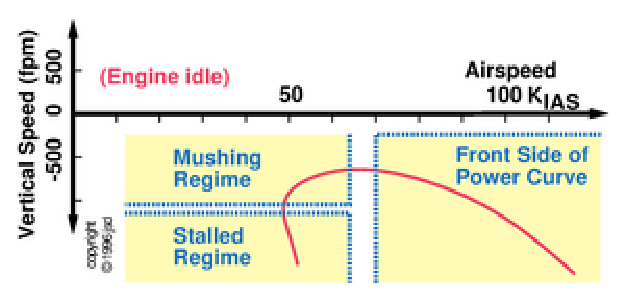
\includegraphics[width=\linewidth]{power-curve-regimes}

We plot airspeed on the X axis and vertical speed on the Y axis. The curve is decidedly not a function: it doubles back on itself. But we can piecewise define it as three functions. We draw a vertical tangent line on the left edge and a horizontal tangent line at the top edge. We'll talk about those tangent points later, they're important. But they define the limits of our three regimes of interest: normal, slow, and stalled. Or as Denker calls them, front side, mushing, and stalled.

Of course, this is at idle power. Since power makes us climb, but the power curve represents a fixed relationship between adjacent speeds that is always the same shape for the airplane, setting power moves the curve up or down. Denker wrote this for a fixed pitch prop, we can instead imagine 55, 65, and 75 percent power.

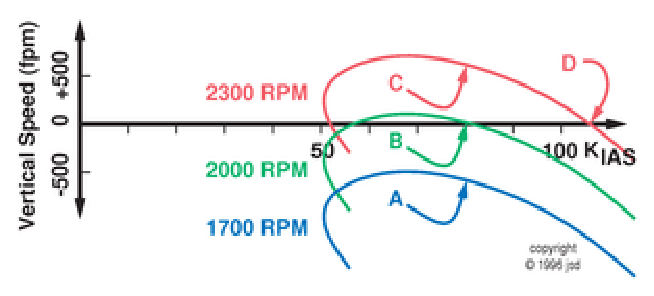
\includegraphics[width=\linewidth]{three-power}

The one gotcha with this explanation of the power curve is that it doesn't really explain what the flaps do directly. But we can derive it. Flaps change the shape of the airfoil and give us more lift in exchange for more drag. Low flap settings give us mostly more lift, high flap settings give us mostly more drag. More lift means moving the curve up. More drag meand moving the curve to the left.

\section{Speed Definitions}

Now that we've built a rigorous framework for describing airplane behavior using the power curve mode, we can go ahead and define some speeds. The following speeds are appropriate for a complex single engine airplane. We do quote the Lance's POH here heavily but I find the POH definitions sorely lacking.

$V_S$ or $V_{S0}$ are the stalling speeds in the cruise or clean configuration: gear up, flaps up. This is the leftmost point on the power curve, the barrier between the stalled and mushing regimes. From the Lance's POH: ``stalling speed, or the minimum steady flight speed at which the airplane is controllable.''

$V_{S1}$ is the stalling speed in the landing or dirty configuration: gear down, flaps down. Since extending the flaps moves the power curve to the left, stalling speed is lowered.

$V_R$ is the rotation speed. Denker suggests a few knots below $V_Y$ unless specifically doing a short or soft field takeoff. In those cases I'd lift off right at or around $V_X$.

$V_X$ is the best \emph{angle} of climb speed, which we use to clear an obstacle. Denker draws a tangent from the origin of his performance curve axes to the power curve, the point of intersection is $V_X$. That speed will get slower if the power curve moves up (more lift) or to the left (more drag).

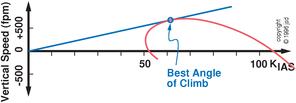
\includegraphics[width=\linewidth]{vx}

$V_Y$ is the best \emph{rate} of climb speed, which we use to gain altitude quickly. It corresponds to the maximum lift over drag speed, meaning, the most efficient point of operation. The maximum endurance speed is usually not far from this value. Denker draws this at the top of the power curve, or rather, where a horizontal line would be tangent to the curve. This does change with weight but as Denker points out the power curve is pretty flat here.

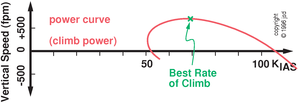
\includegraphics[width=\linewidth]{vy}

$V_G$ is the best glide speed. $V_Y$ is a reasonable guess.

$V_{FO}$ is the flap operation speed. We don't have a specific one for the Lance.

$V_{FE}$ is the flap extension speed. This is the speed at which the flaps may be extended. From the POH: ``the highest speed permissible with wing flaps in a prescribed extended position.''

$V_A$ is the maneuvering speed. It is ``the maximum speed at which application of full available aerodynamic control will not overstress the airplane.'' I talk about $V_A$ in a later chapter, but realize that it depends on weight, and tests \emph{a single control's full deflection at once}. Putting multiple controls to full deflection may overstress the airframe.

$V_{LO}$ is the landing gear operation (retraction) speed. This is the maximum speed at which the landing gear may be safely extended or retracted.

$V_{LE}$ is the landing gear extended speed. It is ``the maximum speed at which an aircraft can be safely flown with the landing gear extended.''

$V_{NO}$ is the ``normal operating'' speed. ``Maximum Structural Cruising Speed is the speed that should not be exceeded except in smooth air and then only with caution.''

$V_{NE}$ is the never exceed speed. Operations past this speed are likely to cause structural damage to the aircraft.

\section{Lift and Weight}

Recall the lift equation:

\begin{equation}
L = \frac{1}{2} \rho V^2 C_L S
\end{equation}

, where $\rho$ is the density of the air, $V$ is velocity, $C_L$ is the coefficient of lift and $S$ is the surface area of the airfoil.

That $V^2$ term is key, Lift is proportional to the \emph{square} of velocity. So what happens if we halve the weight, and thus, the needed lift? Well, it would drop by the square root of a half, which happens to be $\frac{\sqrt{2}}{2} \approx 0.707\ldots$ which is about 29 percent. At three-quarters weight, it drops by the square root of three quarters, which is $\frac{\sqrt{3}}{2} \approx 0.866\ldots$ which is about 13 percent.

Denker points out that the entire power curve shifts up and to the right, with both power off and power on. He even points out a Cherokee Six as a specific example of this - how interesting!

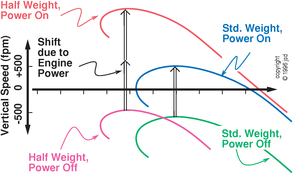
\includegraphics[width=\linewidth]{light-power}

The procedure to derive this curve is as follows:

\begin{enumerate}
\item Scale the entire standard weight, power off curve by the reduction factor. It will move up (since vertical speeds are chopped - a light airplane doesn't sink as much) and to the left (since airspeeds go down - a light airplane has a lower stalling speed).
\item Shift the curve up for power. Realize that, since the airplane is lighter, the curve will shift by a greater amount.
\end{enumerate}

\section{Center of Gravity and Performance}

There are some truths that the private pilot is expected to know about not only how the weight of the airplane affects performance, but also how the center of gravity affects performance.

First we can build some intuition. Fold a paper airplane (technically an ``origami glider''). Go ahead, I'll wait. Now fly it. Observe how it flies. No wrong or right here, just observe the behavior. We'll use this as a baseline.

Now take a paper clip and clip it to the nose. Fly it again. What changes? It's a bit more stable - it wants to fly where we throw it. But it wants to nose down and stops flying at a lower speed. We can make it fly further by bending some tabs in the back.

Now take the paper clip, remove it from the nose, and clip it to the tail. Fly it a third time. What happens? Does it even fly at all? Probably not.

These are the extremes. If we flew a real airplane this nose or tail heavy it would be bad news indeed. But the same truths apply.

A nose heavy airplane is more stable. Why? For the same reason a tightrope walker is more stable holding a stabilizing rod: distribution of weight. The larger arm between the center of gravity (or center of mass - we use the terms equivalently) and the center of pressure means that the weight can act in a more nuanced fashion. The elevator (on a normal airplane with a normal empennage, not some Burt Rutan designed contraption) has to fly heavier to counteract the nose heaviness, which means it has more authority.

With the nose being heavy, the nose wants to keep falling over. We eat into our angle of attack budget because we need to fight to keep the nose up with elevator trim and angle of attack - just like we saw on our paper glider earlier.

The thing about flying with a higher angle of attack is that it increases our drag in all regimes. It increases our induced drag because the plane has to generate more lift at lower speeds. It increases our parasite drag because the frontal area of a wing at a higher angle of attack is greater.

If we take a look at the usual form of the lift/drag diagram - the one out of the testing supplement - some truths about stalling speed and cruise speed become pretty obvious. (But it took ten years for me to think of it this way...)

Compare power available and power required (sum total of induced and parasite drag).

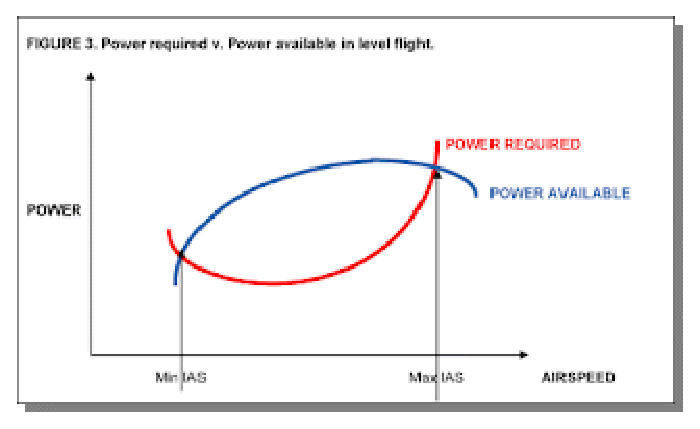
\includegraphics[width=\linewidth]{power-required-available}

Image borrowed from \url{http://airsoc.com/articles/view/id/59acd2623d2d2ebb7e8b4567/behind-the-power-curve} until I make a better one.

This is a different view of the power curve. This form is nice because the stalling and cruising speed of the airplane fall out nicely. They are the places where the red and blue curves intersect. The intersection point on the left is the stalling speed. The intersection point on the right is max cruise.

So what does the higher angle of attack required for a nose heavy airplane do? It moves the red curve UP. What happens to the points? They move \emph{closer together}.

A nose heavy airplane has a \emph{higher} stall speed and a \emph{lower} cruise speed. It is more stable.

Now. What happens to $V_Y$, our best climb speed? It so happens this speed is at $L/D_{max}$, the maximum lift over drag speed. Translating a curve up or down doesn't change that point. So $V_Y$ is \emph{unchanged}.

The converse is true for an aft heavy airplane: lower stall speed (!), higher cruise speed, lower angle of attack, less stable. The red curve moves DOWN.

If we look at the sort of spiral shaped view of the power curve we'd been looking at, a really high angle of attack from a nose heavy airplane would compress the curve about its best rate of climb. So what does this do to $V_X$? Well, recall that we had this clever tangent line definition of $V_X$ erarlier. If we compress the curve, that tangent point \emph{necessarily} moves to the left - as does \emph{every} point on the ``back of the power curve''! So $V_X$ will increase. Slightly.

\section{Altitude and Performance}

For this let's consider a naturally aspirated engine. Turbocharged, supercharged, and turbine engines have different properties.

As the airplane climbs the engine becomes starved for air. The power curve moves down.

What happens to $V_X$? Well we defined it earlier as a tangent point along that power curve. As the curve comes down, the tangent point moves to the right. $V_X$ increases.

How about $V_Y$? We have less excess power at any given airspeed. The curve shrinks a little bit. $V_Y$ slowly increases with altitude because we have less and less excess power.

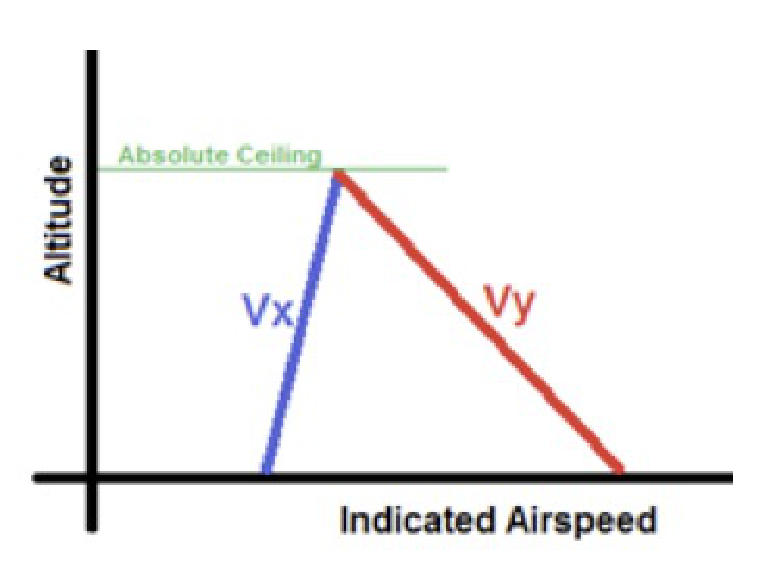
\includegraphics[width=\linewidth]{vx-vy}

See \url{https://www.advancedpilot.com/articles.php?action=article&articleid=1842}. Or for yet another take on this see \url{https://azpilots.org/news/17-safety/50333-climb-speeds}.

As altitude increases, our $V_X$ increases and our $V_Y$ decreases until they converge. At this point we have zero climb performance and one - only and exactly one - point on our power curve produces a nonnegative climb rate. That's our absolute ceiling.

If we're in a pinch and need to find $V_Y$ we can put on our test pilot hats and do so empirically. Set a speed and watch the VSI. Knock 5 knots off (one line on the airspeed indicator). Trim for it and hold it. Are we climbing at a faster or slower rate?

Remember, too, that $V_Y$ cannot go up, unless we swap engines.

\section{V Speeds for the Lance}

The Lance's POH defines a number of speeds. These speeds are commonly defined for single engine airplanes.

In this section, we explore the Lance's V speeds. For each V speed, we consider the definition of the speed, what it means operationally, and how it varies with respect to aircraft weight, aircraft loading (nose or tail heavy), density altitude, aircraft configuration (flaps, landing gear), and aircrat attitude.

The beginning of Section 4 of the POH provides many of these figures.

Recall the weights and speeds variation formula, which we can derive from two different values of the lift formula. It is written here for stall speed but applies to many speeds in this section.

\begin{equation}
V_S' = V_S \sqrt{\frac{New\ Weight}{Old\ Weight}}
\end{equation}

We can use this formula to calculate different speeds for a few different weights. I'll show values for 3600 lbs (max gross), 3200 lbs, 2800 lbs, 2400 lbs, and the airplane's minimum weight (with third row seats removed) of 2151 lbs as per the most recent POH.

Here is a cheat sheet with all the V speeds at max gross weight.

\begin{figure}
\begin{center}
\begin{tabular}{ |c|c|c| }
    \hline
    $V$ Speed & Value (KIAS) & Marking\\
    \hline
    \hline
     $V_{SO}$ &  52 & Bottom of White Arc \\
     $V_S$    &  53 & Bottom of Green Arc \\
    \hline
     $V_R$    &  87 & None \\
    \hline
     $V_X$    &  68-87 & None \\
     $V_Y$    &  92    & None \\
    \hline
     $V_{FE}$ &  109 & Top of White Arc \\
     $V_A$    &  132 & Placard \\
    \hline
     $V_{LO}$ &  106 & Placard \\
     $V_{LE}$ &  129 & Placard \\
    \hline
     $V_{NO}$ &  150 & Bottom of Yellow Arc \\
     $V_{NE}$ &  191 & Red Line \\
    \hline
\end{tabular}
\end{center}
\caption{V Speeds - P32T}
\label{fig:VSpeedsP32T}
\end{figure}

\subsection{$V_{S}$ - Stalling Speed}

52-53 KIAS.

Variation Chart: see Figure ~\ref{fig:StallSpeedsP32T}.

\begin{figure}
\begin{center}
\begin{tabular}{ |c|c| }
    \hline
    Weight & Stalling Speed \\
    (pounds) & (KIAS) \\
    \hline
     3600 &  53 \\
     3200 &  50 \\
    \hline
     2800 &  47 \\
     2400 &  43 \\
    \hline
     2151 &  41 \\
    \hline
\end{tabular}
\end{center}
\caption{Stalling Speed Weight Variance - P32T}
\label{fig:StallSpeedsP32T}
\end{figure}


\begin{itemize}
\item Markings: Bottom of green arc for flaps up. Bottom of white arc for flaps down.
\item Weight: a heavier airplane will require a higher angle of attack to fly and thus will have a higher stalling speed. A lighter airplane will have a lower stalling speed.
\item Loading: a nose heavy airplane will have a higher stalling speed due to the high angle of attack required to keep the nose flying. Conversely, an aft loaded airplane will have a lower stalling speed. But according to Denker the effect is relatively small, a few knots.
\item Density Altitude: In thinner air, there is a greater discrepancy between indicated and calibrated airspeed. The airplane will stall at the same indicated airspeed but a higher true airspeed.  
\item Configuration: Changing the shape of the wings by deploying flaps changes the effective angle of attack. Deploying flaps will usually make the stall speed decrease.
\item Attitude: Stalling speed increases in a turn since we are using a larger component of our lift vector to keep the airplane aloft. In turbulence, the angle of incidence may vary, leading to an earlier stall because the relocation of the relative wind causes us to exceed critical angle of attack earlier. 
\end{itemize}


\subsection{$V_{NE}$ - Never Exceed Speed}

191 KIAS or 189 KCAS

Variation Chart: None. This is an absolute value based on aerodynamic pressure, measured with the pitot tube. The wings and tail can crumple at any weight.

\begin{itemize}
\item Markings: Top of the yellow arc on the airspeed indicator. Red line on same indicator.
\item Weight: No factor.
\item Loading: No factor.
\item Density Altitude: Will occur at a higher true airspeed, but same indicated airspeed, at high density altitude.
\item Configuration: TODO
\item Attitude: TODO
\end{itemize}

\subsection{$V_{NO}$ - Maximum Structural Cruising Speed}

150 KIAS or 150 KCAS

Variation Chart: None. This is an absolute value based on aerodynamic pressure, measured with the pitot tube. The wings and tail can crumple at speeds beyond this in turbulence due to momentary increases in load factor. Operations in this region, including descents, are approved in smooth air. Proceed with caution!

\begin{itemize}
\item Markings: TODO
\item Weight: TODO
\item Loading: TODO
\item Density Altitude: TODO
\item Configuration: TODO
\item Attitude: TODO
\end{itemize}

\subsection{$V_A$ - Design Maneuvering Speed}

132 KIAS or KCAS at max gross weight. Also ``Turbulent Air Operating Speed''.

Variation Chart: Per POH, use linear interpolation to get $V_A$ at various weights. See Figure ~\ref{fig:ManeuveringSpeedsP32T}.

\begin{figure}
\begin{center}
\begin{tabular}{ |c|c| }
    \hline
    Gross Weight & Maneuvering Speed \\
    (pounds) & (KIAS) \\
    \hline
     3600 &  132 \\
     3400 &  129 \\
    \hline
     3200 &  126 \\
     3000 &  123 \\
    \hline
     2800 &  120 \\
     2600 &  117 \\
    \hline
     2400 &  115 \\
     2151 &  112 \\
    \hline
\end{tabular}
\end{center}
\caption{Maneuvering Speed Weight Variance - P32T}
\label{fig:ManeuveringSpeedsP32T}
\end{figure}

\begin{itemize}
\item Markings: Placarded for max gross weight.
\item Weight: TODO
\item Loading: TODO
\item Density Altitude: TODO
\item Configuration: TODO
\item Attitude: TODO
\end{itemize}

\subsection{$V_{FE}$ - Maximum Flaps Extended Speed}

109 KIAS or KCAS

Variation Chart: None. This is a structural limitation.

\begin{itemize}
\item Markings: TODO
\item Weight: TODO
\item Loading: TODO
\item Density Altitude: TODO
\item Configuration: TODO
\item Attitude: TODO
\end{itemize}

\subsection{Maximum Landing Gear Extension Speed}

129 KIAS or 130 KCAS

Variation Chart: None. This is a structural limitation.

\begin{itemize}
\item Markings: TODO
\item Weight: TODO
\item Loading: TODO
\item Density Altitude: TODO
\item Configuration: TODO
\item Attitude: TODO
\end{itemize}

\subsection{Maximum Landing Gear Retraction Speed}

106 KIAS or 109 KCAS

Variation Chart: None. This is a structural limitation.

\begin{itemize}
\item Markings: TODO
\item Weight: TODO
\item Loading: TODO
\item Density Altitude: TODO
\item Configuration: TODO
\item Attitude: TODO
\end{itemize}

\subsection{$V_{LE}$ - Maximum Landing Gear Extended Speed}

129 KIAS or 130 KCAS

Variation Chart: None. This is a structural limitation.

\begin{itemize}
\item Markings: TODO
\item Weight: TODO
\item Loading: TODO
\item Density Altitude: TODO
\item Configuration: TODO
\item Attitude: TODO
\end{itemize}

\subsection{Caution Range - Yellow Arc}

150 KIAS to 191 KIAS

Variation Chart: None. See prior discussion of $V_{NO}$.

\begin{itemize}
\item Markings: TODO
\item Weight: TODO
\item Loading: TODO
\item Density Altitude: TODO
\item Configuration: TODO
\item Attitude: TODO
\end{itemize}

\subsection{$V_Y$ - Best Rate of Climb Speed}

87 KIAS (gear down, flaps up) to 92 KIAS (gear up, flaps up)

Variation Chart: Yes. As this is a speed derived from the power curve, it is subject to translations and scalings of the power curve based on gross weight and configuration. See Figure ~\ref{fig:VYCleanP32T} for the clean configuration and ~\ref{fig:VYDirtyP32T} for the dirty configuration. I consider these speeds to be optimistic and generally add 2-3 knots.

\begin{figure}
\begin{center}
\begin{tabular}{ |c|c| }
    \hline
    Weight & Speed \\
    (pounds) & (KIAS) \\
    \hline
     3600 &  92 \\
     3200 &  87 \\
    \hline
     2800 &  81 \\
     2400 &  75 \\
    \hline
     2151 &  71 \\
    \hline
\end{tabular}
\end{center}
\caption{Best Rate of Climb Speed Weight Variance, Clean - P32T}
\label{fig:VYCleanP32T}
\end{figure}

\begin{figure}
\begin{center}
\begin{tabular}{ |c|c| }
    \hline
    Weight & Speed \\
    (pounds) & (KIAS) \\
    \hline
     3600 &  87 \\
     3200 &  82 \\
    \hline
     2800 &  77 \\
     2400 &  71 \\
    \hline
     2151 &  67 \\
    \hline
\end{tabular}
\end{center}
\caption{Best Rate of Climb Speed Weight Variance, Dirty - P32T}
\label{fig:VYDirtyP32T}
\end{figure}

\begin{itemize}
\item Markings: TODO
\item Weight: A higher weight causes a higher angle of attack and leaves less power available resulting in a higher best rate of climb speed.
Variation Chart: TODO
\item Loading: No variation. None! A nose heavy airplane will have higher induced drag and require more power to overcome this greater induced drag.
The POH provides a hint concerning takeoff performance for nose heavy CGs forward of 85 inches. This increase is due to the gadded drag of the nose heavy airplane.
\item Density Altitude: TODO
\item Configuration: TODO
\item Attitude: None. Attitude follows takeoff configuration, not the other way around. Fly coordinated now.
\end{itemize}

\subsection{$V_X$ - Best Angle of Climb Speed}

68 KIAS (gear down, flaps up) to 87 KIAS (gear up, flaps up)

Variation Chart: Yes. As this is a speed derived from the power curve, it is subject to translations and scalings of the power curve based on gross weight and configuration. See Figure ~\ref{fig:VXCleanP32T} for the clean configuration and ~\ref{fig:VXDirtyP32T} for the dirty configuration. I consider these speeds to be optimistic and generally add 2-3 knots.

\begin{figure}
\begin{center}
\begin{tabular}{ |c|c| }
    \hline
    Weight & Speed \\
    (pounds) & (KIAS) \\
    \hline
     3600 &  87 \\
     3200 &  82 \\
    \hline
     2800 &  77 \\
     2400 &  71 \\
    \hline
     2151 &  67 \\
    \hline
\end{tabular}
\end{center}
\caption{Best Angle of Climb Speed Weight Variance, Clean - P32T}
\label{fig:VXCleanP32T}
\end{figure}

\begin{figure}
\begin{center}
\begin{tabular}{ |c|c| }
    \hline
    Weight & Speed \\
    (pounds) & (KIAS) \\
    \hline
     3600 &  68 \\
     3200 &  64 \\
    \hline
     2800 &  60 \\
     2400 &  56 \\
    \hline
     2151 &  53 \\
    \hline
\end{tabular}
\end{center}
\caption{Best Angle of Climb Speed Weight Variance, Dirty - P32T}
\label{fig:VXDirtyP32T}
\end{figure}

\begin{itemize}
\item Markings: None.
\item Weight: A lighter airplane has a lower $V_X$. A heavier airplane has a higher $V_X$. See previous discussion.
\item Loading: A nose heavy airplane has a slightly higher $V_X$. See previous discussion.
\item Density Altitude: TODO
\item Configuration: TODO
\item Attitude: None. Attitude follows takeoff configuration, not the other way around. Fly coordinated now.
\end{itemize}

\subsection{Landing Final Approach Speed, Full Flaps}

75 KIAS

Variation Chart: TODO
\begin{itemize}
\item Markings: TODO
\item Weight: TODO
\item Loading: TODO
\item Density Altitude: TODO
\item Configuration: TODO
\item Attitude: TODO
\end{itemize}

\subsection{Maximum Demonstrated Crosswind Velocity}

17 knots.

Variation Chart: None.

\begin{itemize}
\item Markings: TODO
\item Weight: TODO
\item Loading: TODO
\item Density Altitude: TODO
\item Configuration: TODO
\item Attitude: TODO
\end{itemize}

%
%\subsection{$V_V$ - Speed Speed}
%Variation Chart: TODO
%\begin{itemize}
%\item Markings: TODO
%\item Weight: TODO
%\item Loading: TODO
%\item Density Altitude: TODO
%\item Configuration: TODO
%\item Attitude: TODO
%\end{itemize}
%

\section{Limitations}

Along with performance, we need to understand the limitations of the aircraft. This section focuses on the Lance's limitations as mentioned in the POH, Section 2. It references the performance charts in the Lance's POH. We also need to cross-reference Section 9, the Supplements, for optional equipment. The writeup here focuses on things that the pilot can control or needs to know, and not things that are set on the ground (like the propeller diameter).

\subsection{Airspeed}

We discussed the airspeeds extensively in the previous section.

\subsection{Engine}

Maximum RPM: 2700.

Maximum oil temperature: 245 F (POH figure) or 118 C.

Oil pressure: minimum 25 PSI (red line), maximum 100 PSI (red line). We do exceed this briefly on the ground when oil is cold regularly by about 5 PSI.

Fuel pressure: minimum 12 PSI, maximum 40 PSI.

Fuel grade: 100/130 - Green. We use 100LL - Blue in the airplane all the time.

\subsection{Weight Limits}

Maximum weight of the airplane is 3600 lbs. Maximum baggage is 200 lbs, with 100 lbs in each of the fore and aft compartments.

\subsection{Center of Gravity}

At 3600 lbs: CG from 91.4 to 96.0 inches aft of datum.

At 3000 lbs: CG from 84.0 to 96.0 inches aft of datum.

At 2500 lbs: CG from 82.0 to 96.0 inches aft of datum.

\subsection{Maneuvers}

No acrobatics. No spins.

\subsection{Flight Load Factors}

Positive load factor to 3.8G - this is a ``Normal'' category airplane.

No inverted maneuvers approved.

\subsection{Types of Operations}

Day and Night VFR and IFR. Non icing.

\subsection{Fuel Limitations}

98 gallons total, of which 4 gallons are unusbale and 94 gallons are usable. These are totals, divide in half for each wing.

\subsection{Rear Cabin Door Removal}

Such operations are authorized. Max speed 144 KIAS. No smoking. Articles and lines must be tied down, stowed, and kept clear of controls and control surfaces. VFR only.


\section{Performace}

Performance and limitations go hand in hand. In this section we take a closer look at performance.

``Remember: to get chart performance, follow the chart procedures.''

\subsection{Airspeed System Calibration}

Recall that calibrated airspeed is indicated airspeed corrected for installation and instrument errors.

The correspondence between KIAS and KCAS is largely linear. There is a slightly less linear region below max lift/drag speed.

Putting the flaps full down introduces about 2-3 knots of calibration error.

The reported calibration is at max gross weight.

There is no indication that calibrated airspeed varies with weight. Since we're simply concerned with the pressure differential in the pitot-static system, the weight should be no factor. If the airplane were infinitely heavy (tied down) the indications would be the same as if the airplane were neutrally buoyant (hovering just above the ground).

\subsection{Stall Speed versus Angle of Bank}

There is a well known correspondence between load factor and stall speed. This chart draws the correspondence between angle of bank, in degrees, and the stall speed with the flaps full down or the flaps full up.

Looking at the chart, we can tell that the airplane's stall speed with the flaps down is one knot lower.

The chart calls out maximum gross weight. As we know from earlier, the stall speed of the airplane varies with loading, which would cause the curve(s) to translate downward as stall speed lowers with reduced weight.

The chart does not provide stall speeds for bank angles beyond sixty degrees. Thus, we could take this to mean that a sixty degree bank is an operational limitation.

\subsection{Flaps Second Notch Takeoff Performance and Ground Roll}

This chart tells us our takeoff distance over a fifty foot barrier as a function of outside air temperature, pressure altitude, weight, and wind.

The chart numbers assume wide open throttle 2700 RPM, holding the brakes, and a paved, level, dry runway. They implicitly assume aft trim since the short field procedure calls this out.

We are cautioned that a nose heavy airplane has a harder time taking off. ``Takeoff distance is increased by approximately 25\% at CGs forward of 85 inches.'' 

The chart is divided into three sections. The relations are decidedly nonlinear, but they are at least first and second order smooth.

In the first section we are in effect calculating the density altitude based on pressure altitude and outside air temperature. Lower temperatures result in shorter takeoff distances (air is more sense). Lower pressures also result in shorter takeoff distances.

In the second section we are correcting for airplane weight. A lighter airplane takes off in less distance (less lift required).

In the third section we are correcting for wind. A headwind reduces takeoff distance. A tailwind increases takeoff distance.

I do not believe the borders of this chart to be regulatory. Certainly we can launch an airplane into a greater than 15 knot headwind, or even a 5 knot tailwind (not something I would want to do without quite a lot of runway). We should be able to take off at pressure altitudes above 7000 feet as well. But doing something off the borders of the chart would certainly give me pause.

For the record, these numbers are extremely optimistic. The chart gives lift off speeds of 62-63 knots and obstacle clearing speeds of 62-65 knots, varying by weight in what now is the usual manner. But in my airplane we're not off until 73 knots at the earliest. That is a 15\% discrepancy. So I make sure to pad these numbers by 15\% in my own operations.

The ground roll chart is largely identical to the prior chart. All of the prior discussion applies, including the caveats. The main difference is that we are calculating ground roll instead of distance over an obstacle.

\subsection{Flaps Up Takeoff Performance and Ground Roll}

This chart is the bread and butter of our operations. Most of our takeoffs will be normal. The discussion from the flaps second notch charts applies here as well.

The liftoff speeds, once again, are optimistic. They say we will be off at 66-70 knots. I find that hilarious. N36262 doesn't want to fly until about 85 knots, you can't even pull it off the ground without some difficulty. That's a 25\% discrepancy, and I would add a 25\% ``fudge factor'' to these figures.

\subsection{Gear Up and Gear Down Rate of Climb}

This chart provides the climb performance of the airplane as a function of density altitude, engine fuel mixture, and airplane weight. The climb rate may be zero, or as great as 1700 feet per minute according tot his chart.

To achieve these numbers, the provided configuration is: gear up or down, flaps up, mixture as noted, wide open throttle, maximum RPM of 2700, and $V_Y$, which is once again 92 (gear up) or 87 (gear down) knots indicated.

These numbers are optimistic as well. They imply a 16,000 foot service ceiling for the airplane. That's very interesting as I saw a demonstrated service ceiling of 12,500 feet on an ISA+05 day, seeing about 50-100 feet per minute when we should have been seeing 200 according to this chart. So I would knock off 100 to 200 feet per minute - I would shift the entire right hand section of these charts over to the left a little bit.

\subsection{Fuel, Distance, and Time to Climb}

This chart estimates the fuel (in gallons), time (in minutes) and distance (in nautical miles) to achieve a particular density altitude. We collect data at the density altitude of takeoff, and of cruise, and take their difference to get our expected performance.

As usual, these numbers are so optimistic as to be objectionable.

The numbers are given in this configuration: gear up, flaps up, 2700 RPM, full throttle, 92 KIAS, 3600 lbs gross weight, no wind.

My procedure is to pull the engine back to 2500 RPM once we're at least 500 AGL. The primary reason for this is noise abatement. The secondary reason is to reduce wear and tear on the engine. The Cirrus derates the engine to 2500 RPM. That costs some performance.

But do leave the throttle alone. We don't need to pull it back. It's just one more thing to mess with in a critical phase of flight.

John Deakin talks about engine performance on takeoff here: \url{https://www.avweb.com/features/pelicans-perch-63where-should-i-run-my-engine-part-1/} and \url{https://www.avweb.com/features/pelicans-perch-64where-should-i-run-my-enginepart-2-the-climb/}. These are part of the truly excellent \emph{Pelican's Perch} series of articles he wrote twenty years ago (!). [TODO: Add these articles to the bibliography, copy to the Takeoff section.]

As long as EGTs and CHTs are happy, with our GAMIjectors, we can lean to our heart's content. So I would pull the mixture back a little bit on climb out, and of course continue leaning as we climb into thinner air.

A 15-20\% correction is what we've been using, so maybe that's appropriate here as well.

This chart does not provide any limitations.

\subsection{Power Setting Table}

This chart provides expected RPM and manifold pressure values for 45, 55, 65, and 75 percent engine performance at a number of pressure altitudes. In practice, the engine computer helps us with these values. Note that in a number of situations ``over-square'' valies are explicitly okay, further debunking the square myth.

We add 0.18 inches of manifold pressure for every 10 degree Fahrenheit variation above standard (since we need more air). We subtract for temperature below standard.

The implicit limits of this chart are wide open throttle or stalling the engine.

\subsection{Cruise Performance}

A handful of charts collectively describe speed, power, range, and endurance in a number of cruise configurations. The fuel flows are excessive, with our GAMIjectors we can achieve these numbers about two gallons per hour lower.

\subsection{Fuel, Distance, and Time to Descend}

Much of the discussion for the analogous Climb chart applies here. The configuration specified is: Gear up, flaps up, power as required, 150 KIAS, 500 FPM, 3600 lbs gross weight (which is impossible, we burned fuel to get to this altitude and we didn't refuel in flight), no wind.

\subsection{Glide Range}

The glide ratio is decidedly linear.

The chart gives this configuration for best glide: Gear up, flaps up, $V_Y$ of 92 KIAS, power off, max gross weight (a lighter airplane glides further), propeller full decrease, no wind.

In real life, if the engine quits, you're losing oil pressure and thus governor authority not long after. In a single, the prop defaults to high RPM and acts as an air brake.

\subsection{Landing Performance and Ground Roll}

These charts are similar to the takeoff charts. But, since they assume a power off configuration, they omit a power section.

The associated conditions are: power off approach, full flaps, max gross weight (a lighter airplane stops in less distance), landing gear extended, 75 KIAS approach speed (appropriate for short field technique), full stall touchdown, maximum braking, paved level dry runway.

Performance charts are provided for the ``Optional Landing Gear Heavy Duty Group No. 1''. According to the equipment list, N36262 \emph{DOES} have these installed. These include a Cleveland Aircraft Products 40-120 wheel assembly, 30-82 brake assembly, and Type III tires with eight plies. With stronger brakes, we can reduce the ground roll some.

As usual, I like a 10-20\% margin here.














\chapter{Emergency Procedures}

Dealing with emergencies is a crucial part of operating any aircraft. As a commercial pilot, operations that push the comfort zones and limits of both the pilot and the aircraft will become that much more common. Further, abiding by the law of large numbers, accidents are more likely to happen with more hours in the aircraft. Thus it is critical to be familiar with general emergency procedures, as well as the specific procedures for the airplane. Like the rest of this book, this chapter focuses on the Piper Lance II, P32T.

Systems knowledge, and systems familiarity, play a large role in emergency procedures. Not every emergency will have a dedicated checklist or flow. Sometimes, the pilot may be required to think, slow down, and understand the situation.

The heart of all emergency procedures comes down to this list, provided by Mr. Roger Sharp:

\begin{enumerate}
\item What can go wrong?
\item How would I know?
\item How do I fix it?
\item If I can't fix it, how do I minimize impact?
\end{enumerate}

The first question involves some knowledge of aircraft systems. Thus, unlike the procedures in the POH, this chapter will focus more heavily on systems knowledge as it relates to emergency procedures.

The second question involves knowledge of general aerodynamics as well as the systems and quirks of the particular aircraft.

The third question involves following book procedure.

The fourth question involves aeronautical decision making, or ADM.

\section{Landing Gear}

\subsection{System Overview}

For starters, we begin reading about the landing gear in Chapter 7 of the POH. ``The Lance II is equipped with a retractable tricycle landing gear, which is hydraulically actuated by an electrically powered reversible pump. The pump is controlled by a selector switch on the instrument panel.''

The Landing Gear Electrical Schematic (Figure 7-5) provided an overview of the electrical systems connected to the gear. The landing gear actuator circuit breaker is a 25 amp circuit breaker which regulated the hydraulic pump motor, which is connected via relays to the actuator handle. The Gear Unsafe lamp is wired to the gear actuator and the up limit switches on each gear. The left, nose, and right bulbs are wired directly to the down lock switches.

Though not called out as such in the POH, the ``three greens'' pull right out of the instrument panel in case we need to swap them during emergency operations.

We do have a checklist for the landing gear in Section 3, Emergency Procedures. However, the title of the checklist, ``Emergency Landing Gear Extension'', is something of a misnomer. I would rename it to ``Landing Gear Malfunctions''.

Our airplane, thankfully, has the landing gear auto-extension system deleted. It is safe to ignore any sections of the POH that mention it. I confirmed this explicitly with Piper.

\subsection{Landing Gear Malfunctions - Checklist}

Prior to emergency extension procedure:

\begin{itemize}
\item Master Switch: Check ON.
\item Circuit Breakers: Check.
\item Radio Lights: Off (in daytime).
\item Gear Indicator Bulbs: Check.
\end{itemize}

If landing gear does not check down and locked:
\begin{itemize}
\item Airspeed: Below 87 KIAS.
\item Landing Gear Selector: Down.
\item Emergency Gear Lever: Override Engaged (while fishtailing airplane).
\end{itemize}

If landing gear still does not check down and locked:
\begin{itemize}
\item Emergency Gear Lever: Override Engaged (while fishtailing airplane).
\end{itemize}

If all electrical power has been lost, the landing gear must be extended using the above procedures. The gear position indicator lights will not illuminate.

\subsection{Landing Gear Malfunctions Discussion}

The POH, Section 3.27, provides a short discussion of the above checklist I find this discussion insufficient. So, I will expand upon it here.

The first part of the checklist involves dealing with electrical issues. After all, the hydraulic gear system has an electrical pump that actuates it. Maybe the master switch is off. Maybe the pump burned out.

On this airplane, the radio dimmers also dim the three greens of the landing lights. The suggestion to turn the radio lights off makes certain that the bulbs will be as bright as possible.

The POH says to ``check the landing gear indicators for faulty bulbs''. But it doesn't dare describe \emph{how} to do this. Fro crying out loud. They pull right out of the panel, and can be swapped. Note, from the electrical diagram, that the lights do offer some modicum of redundancy.

Has the airplane been flying in icing conditions? It's possible that the landing gear is frozen into place. Check the outside air temperature gage and fly into an area that has temperatures warm enough to melt the ice if able.

The recommendation to slow down - interestingly, to $V_Y$ in the dirty configuration (it would be helpful if they mentioned that in the POH) - is to pull aerodynamic drag off a weak mechanism.

The recommendation to fishtail the airplane is to help swing a faulty landing gear into place to lock it. But this will only work with the main gears. With the nose gear, some nose dives and recoveries may help to snap the gear into place.

If none of these procedures work, it's helpful to get some eyes on the ground to have a look. Phone a friend, call the tower, or go somewhere else. If it's night time - go to a big airport, maybe they have search lights. A big airport will have more runways and more emergency services. You did bring a 45 minute reserve, did you not?

At this point, it's time to consider a forced landing. Gear up or gear down? That is the question. With two wheels down out of three we can attempt a landing. Try to use aileron or elevator to keep pressure off of the ``bad'' tire for as long as possible, and expect a severe yawing or pitching moment when it finally does catch. Try to turn the engine off to minimize damage.

The POH does not give any specific guidance for a partial gear landing. It DOES give guidance for whether to attempt a power off landing with gear down or gear up. But it doesn't tell us to look there, now does it? The guidance in both cases is the same: lowest possible airspeed with full flaps, ignition off, master switch off, fuel selector off, mixture idle cutoff. Tighten seat belts and shoulder harnesses. I would also open the door and prop it with a jacket, and be ready to evacuate immediately. If there is time, I would prep the fire extinguisher.










\chapter{Weather}

Much as a submarine flies through the water, so too does an airplane fly through the air. Think of the atmosphere as a diverse, swirling, active mix of fluids - gases - creating pressure differentials and swirls and vortices and other phenomena. Weather is simply the study of these phenomena.

Once upon a time the authority on the FAA's weather resources was \href{https://www.faa.gov/regulations_policies/advisory_circulars/index.cfm/go/document.information/documentID/1030235}{AC 00-45H - Aviation Weather Services - Change 2}. As of 2022-12-22, that document is cancelled, in favor of the all encompassing \href{https://www.faa.gov/regulationspolicies/handbooksmanuals/aviation/faa-h-8083-28-aviation-weather-handbook}{FAA-H-8083-28, Aviation Weather Handbook}. That document is a primary reference for this chapter.

The new Handbook incorporates information from a number of now cancelled advisory circulars:

\begin{itemize}
\item AC 00-6, Aviation Weather.
\item AC 00-24, Thunderstorms.
\item AC 00-30, Clear Air Turbulence Avoidance.
\item AC 00-45, Aviation Weather Services.
\item AC 00-54, Pilot Windshear Guide.
\item AC 00-57, Hazardous Mountain Winds.
\end{itemize}





\chapter{Aeromedical Factors}


\chapter{High Altitude Operations}

In this chapter, we introduce high altitude operations.

Before we dive in, we must answer a couple of questions.

What are high altitude operations? Simply put, these are operations far outside the ``normal'' environment you might expect to find on a Standard Day at sea level. We're talking about altitudes that are not terribly comfortable for humans, and possibly altitudes that are so high above MSL that we won't find any terrain there at all. There are enough aeromedical factors and enough changes to aircraft performance that we need to consider these operations carefully.

Why do we care about high altitude operations? We might need to get high enough to cross some mountains and stay above terrain. But there is also the desire for speed. I'm not just talking about the speed limit of 250 knots below 10,000 feet - if we wish to go faster, we need to go higher. I'm talking about the fact that \emph{thinner air provides less drag}, which permits us to fly through the air more efficiently.

Mother Nature, of course, exists outside the realm of aviation. The challenges of high altitudes were present well before the first powered flights - just ask anyone who tried to climb Mount Everest in the 1800s. So, first, we must have a look at the atmosphere itself.

\section{The Atmosphere and Its Layers}

Recalling the basics from aviation weather, we know that the atmosphere is divided into several layers. Starting from the ground and going on up, we have the troposphere, the stratosphere, the mesosphere, the thermosphere, and the exosphere. All weather - and most of the earth's air! - reside in the troposphere. Flight operations rarely venture into the stratosphere (even more rarely now that Concorde is no longer flying).

So, when we say ``high altitude'', we mean ``higher than a short cross country flight but lower than Concorde''. We're talking altitudes below about 45,000 feet. If you ever manage to get above that, please let me know. (I'm looking at you, astronaut friends... you know who you are!)

\section{Density and Altitude}

In order to better talk about the atmosphere, can we all agree on a make believe, consistent, common, daresay, \emph{standard} atmosphere?

Well, apparently, we can. Aviators are all too familiar with the International Standard Atmosphere. This aviator only recently learned that when we say standard, we mean Standard, namely, International Standard (ISO) 2533 from 1975, which is identical to the ICAO Standard Atmosphere from -2 to 32 km, or up to about 100,000 feet.

Assuming you've paid the 198 CHF fee, or can otherwise access the standard, you would see an interesting thing happening. You would see the value of p, the pressure, and $\rho$, the density of the atmosphere, decrease as altitude increases - and rapidly at that. At sea level (zero elevation), pressure is the all too familiar 1013.25 hectopascals. At 3,000 meters or about 10,000 feet, we're down to 701.21 hectopascals - only 69\% of the pressure at sea level! That means 69\% as much air, 69\% as much oxygen available for breathing or combustion, 69\% as much drag.

Up at 10,000 meters or about 33,000 feet - typical airliner altitudes - we're down to 262 hectopascals. That's just over 25\% of the pressure at sea level.

This is a huge change! It's enough that we need to pay special attention to how we are powering our airplanes, how we are providing our bodies with oxygen, and how we are constructing our airplanes. It's enough that we need to take into account certain operational considerations.

\section{Propulsion}

One of the problems with high altitude flight is that the air is so thin, there may not be enough oxygen for the (internal combustion) engine to run properly.

Recall that a normally aspirated aircraft with a piston engine has a service ceiling. That ceiling is defined as the altitude at which the airplane's climb rate slows to 100 feet per minute \cite{marchman}. That exact altitude will vary based on aircraft loading and how the conditions compare to a standard day. Famously, Concorde would continue to climb while underway, going higher as it got lighter. But the fact remains: for a piston airplane, we can only go so high.

Since the limitation is oxygen, and not fuel, there are a few ways that we could gain power at a higher altitude.

What if we had an electric aircraft? That would be great - it doesn't need oxygen at all. Today, in 2022, battery technology isn't quite there, nor are solar cells, outside from a very few research aircraft.

What if we simply had supplemental oxygen on board? Certainly, if we carried oxygen tanks, we could supplement the oxygen in ambient air to gain more power. Operationally, this is not a great idea, since we now have to deal with the added weight, complexity, and risk of an oxygen system, and it will not last very long. But air-breathing rockets do exactly this, so it's not a bad idea per se, simply not the right one.

What if we could grab more air from the atmosphere, possibly by compressing the air before it gets to the engine intake manifold? Now we're on the right track.

The first approach we might take is simply inserting a compressor between the outside air intake and the engine's intake manifold. That compressor could be a piston pump, similar to the vacuum pum in the airplane. But that's not terribly efficient: it generates a fair amount of waste heat. For this application, a turbine is a better idea. We could power this compressor with the aircraft's engine, most likely with a belt or a gear drive off the engine crankshaft. Such a contraption has a name: supercharger. It requires more power from the engine, and there are some losses due to the belt or gear drive mechanism, but it is a new positive up to a point: we can shove more oxygen into the engine, and raise our service ceiling.

Some clever person (who?) looked elsewhere on the engine and found another possible source of energy for driving this compressor. They realized that the exhaust gasses coming out of the engine were quite warm and under a decent amount of pressure. What if this energy could be captured? We can add a \emph{second} turbine in line with the exhaust pipe, and use the torque generated by that turbine to drive our intake compressor! As it turns out, this works better than a supercharger. We call this a ``turbocharger''. Sometimes we have more than one.

(some diagrams should go here)

Operating a supercharged or turbocharged engine has some key differences from operating a normally aspirated engine. One, we need to re-calibrate our manifold pressures. By this I mean, in normal operation, a piston engine's intake manifold would achieve a pressure no higher than ambient pressure, likely no more than 32 inches of mercury. But, a turbocharged (or supercharged) engine may be able to go above this. I say ``may'' because some turbos simply give sea-level pressure at higher altitudes (turbonormalized), whereas others can go well above sea level pressure. Regardless, the turbo lets the engine run harder than it could otherwise, which means increased heat and risk of engine damaged. There are often limitations on how long an engine may run on a particular power setting as a result.

The turbocharger (or supercharger) turbines are themselves metal parts that are subject to fatigue and thermal stresses. After flights, we want to give the turbines some time to cool down, lest we shut them off entirely and subject them to thermal shock.

Recall that, when we compress air, it gets quite warm. This is unfortunate, since we recall from the application of carburetor heat that warm air will lean our mixture. What if there were a way to compress the air, and then cool it to get it as dense as possible? There is: it is called an ``intercooler''. But, as this requires even more heat to be dissipated from the aircraft, the intercooler must be carefully placed so that it can dissipate heat effectively.

With a turbocharged engine in particular, the concept of ``exhaust gas temperature'' takes on a new meeting. Where are we measuring: before the exhaust turbine, or after? It makes more sense to measure before, and we call this the ``turbine inlet temperature'' or TIT. We need to manage this temperature carefully: we want the TIT to be as high as possible for efficient leaning of the engine, but if it is too high, it could melt the exhaust turbine.

These turbines need to spin quite fast - think 100,000 RPM - in order to be effective. It is challenging and expensive to create machinery that can operate at this speed.

All of this seems awfully complicated for a little bit of extra power. What if there was a better way?

There is. It's called the jet engine.

The jet engine is, at is simplest, a single turbine. It ingests air and compresses it. We inject fuel into the compressed air and ignite it, causing it to heat and expand. The exhaust heats and expands so much that it exerts a force on a turbine, which serves as thrust for the airplane. Much like the turbocharger, the jet engine grabs some energy from the exhaust system to power the input compression phase.

More specifically, this single arrangement is called a "turbojet". It is simple, powerful, and reliable. So long as fuel usage and noise are of no concern, this is the best powerplant. The military often doesn't care about fuel or noise so we see turbojets on plenty of military aircraft. If we care more about efficiency and noise than (potentially supersonic) speed, we can also attach a really fast-spinning propeller to this, and capture the propeller's thrust in a duct for maximum efficiency. This combination of a turbojet with a ducted fan is called a "turbofan" and is the most popular way of powering large aircraft.

Of course, the propulsion system allows the aircraft to operate at a higher altitude. But what about the pilot, flight crew, and passengers? Do we need to do anything special for them if we are flying at high altitudes?

\section{Aeromedical Factors}

Much like the airplane's engine, the human body needs a certain amount of oxygen to perform.

\subsection{Hypoxia}

\subsection{Diving and Flight}

\subsection{Humidity}

\section{Supplemental Oxygen Systems}

\section{Operational Considerations}



\chapter{The Commercial Pilot}

So you want to become a commercial pilot? What are the privileges and limitations for such a pilot? What does that even mean?

One thing is for certain: the private pilot checkride is NOT simply a ``glorified commercial pilot checkride''. The expectations - and risks - for a commercial pilot are much higher.

Think of it this way. The private pilot checkride represents your first flight with a passenger (albeit a fairly picky one at that). The commercial pilot checkride is meant to simulate your first \emph{job interview} as a pilot. It's all about professionalism, polish, and positive control.

The private pilot checkride is your change to demonstrate competence. The commercial pilot checkride demonstrates fluency, professionalism, experience, and finesse. Of course, the ATP checkride takes this to another level, but we'll talk about that another day.

The PHAK \cite{PHAK} is a great reference. So is the AFH \cite{AFH}. It's good for commercial pilots to be familiar with hazardous attitudes \cite{adm} as well.

\section{Training}

The Commercial Pilot is held to a higher standard than the Private Pilot. Many of the maneuvers on the private pilot checkride make an appearance on the commercial pilot checkride as well. Quantitatively, the commercial pilot has less margin: tighter limits for airspeed, altitde, heading, bank, landing distance, etc. Qualitatively, the checkride examiner wants to see that the commercial pilot candidate is the clear master of the aircraft. They are looking for positive control, smoothness, rudder coordination (and cross-coordination when appropriate!), and appropriate use of trim or checklists.

With the private pilot we ask, would I trust the candidate to take my spouse or child flying? With the commercial pilot we ask, would I trust the candidate to take my entire family flying? Are they the clear master of the aircraft? Can they explain the aircraft's, as Doug De Muro would say, quirks and features? Do they make the airplane do what they want it to do, when they want it, for reasons they can clearly explain?

For the author, the process of commercial pilot training was humbling. I already had about 100 hours in my airplane, was already instrument rated, and felt like a safe, competent pilot. How hard could it possibly be? I thought I could knock out the training in about five hours of dual instruction (in addition to all the other requirements in 14 CFR 61.129 of course). I thought wrong.

Commercial pilot training forced me to be a student pilot again. It was frustrating. It was humbling. I was practicing many of the same things that I had already demonstrated as a private pilot, but in a larger, faster airplane that was not a Cessna 172. (The author feels that there is an implicit bias toward the Cessna 172 in pilot training materials.) I was being forced to look outside - after learning to fly as an instrument pilot. I was being asked to put G forces on my body and airplane that were not necessarily comfortable, and would be extremely concerning in an instrument environment. Not only was I having to re-learn things that I had previously learned in a different airplane with a different instructor, but I was also being held to a higher standard. That standard, of course, is the Commercial Pilot ACS \cite{acs-commercial}.

The ``good news'', at least for me, was that I was not immediately dependent on passing my checkride to gain any new privileges. I didn't have an airline job lined up. I could still fly myself and my family around if I wanted to. After some initial frustration, I learned to re-embrace the learning process, and that it's okay to postpone a checkride once, twice, or even more times. Cancellations are free, but disqualifications will cost you.

If I were to go back in time, and talk to myself when beginning, I would offer the following pieces of advice:

\begin{itemize}
    \item This is going to take longer than you expect.
    \item This is VFR training with an instructor. Schedules, airplane maintenance, and weather all need to align. Often times they won't.
    \item For every hour in the air, spend three hours on the ground, split evenly between debriefing the previous flight and preparing for the next flight.
    \item Try to remember to have fun with this! Flight training is an incredible privilege that not everyone is able to do.
    \item Just because examiners book a month out doesn't mean you need to book immediately. A concrete date can be a good thing (motivation) and a bad thing (an unnecessary stressor).
    \item The difficulty of commercial pilot training is a direct function of competency at the end of the private pilot checkride. If soft and short field operations, steep turns, and emergency descents remained regular operations, things will go easier. If, however, it has been two years since the words ``steep turns'' came out of your mouth, this might take a little while.
\end{itemize}

Ultimately, my own goals include being a flight instructor (for which the commercial rating is a prerequisite) and being competent in my airplane (commercial training certainly explores the flight envelope).

\section{Ground Operations}

TODO. Spend some time talking here about what makes a commercial pilot more senior than a private pilot on the ground. Do so in ACS order. Talk about airworthiness requirements, weather information, cross country flight planning, the National Airspace System, Performance and Limitations, Operation of Systems, Human Factors, Preflight Assessment, Flight Deck Management. This ends up reading like a checkride cheatsheet.

\subsection{Engine Starting}

At the commercial pilot we kick everything up a notch, even something as humdrum as starting the engine. Surely we've started an ending before?! But now, we should be able to talk a little more about what's going on.

TODO: talk about how in starting the engine, the prime makes the fuel mixture rich, and cranking makes the mixture progressively leaner until we catch.

TODO: talk about gear driven starters and how to not damage them.

TODO: discuss whether or not to leave the alternator on while starting. Depends on POH. Belt vs gear driven alternators.

TODO: discuss importance of ground lean.

\subsection{Taxiing}

On the checkride, make sure to use an appropriately slow taxi speed. Rushing on the ground will only make the checkride end faster by getting you disqualified. 10 knots is a good ground speed. Feet off the brakes and minimal RPM for this. Don't forget crosswind controls.

\subsection{Before Takeoff Check}

Follow the checklist.

What would you do if the engine ran rough?

Takeoff briefing. Describe what we would do if there were an obstruction on the runway. What kind of takeoff is this? Where do we expect to be airborne? What do we do if our engine quits on the ground roll? On rotation? At 100 AGL? At 500 AGL? Making a 360 is a bad idea. Making a 180 might be a good idea. Using a crosswind runway is an option. Maybe scope out landing sites just off the departure end of the runway ahead of time.

The Lance has an STC for GAMIjectors, which explicitly allow us to lean the mixture to peak EGT for takeoff. I use this as my justification for leaning the mixture to get the RPM drop in the mag check to where I need it to be. At this point, in the Lance, I might point out that the D in Lycoming IO-540-K1G5D stands for ``dual magneto'', meaning both magnetos are driven by a single gear. This is a single point of failure for the magnetos, which is an unfortunate design.

\section{Flight Operations}

The Commercial Pilot ACS \cite{acs-commercial} is the bible for the Commercial Pilot checkride. We refer to it frequently in this section.

The author has, as of this writing, spent the most time in the P32T type, a T-tailed Piper Lance II. The detailed procedures here implicitly refer to the Lance, and its airspeeds and quirks. Some details will differ based upon the particular aircraft.

The Lance has a wide range of flight envelopes. It flies very differently when nose loaded with a forward center of gravity (CG), as opposed to when aft loaded with a rear CG. The numbers and profiles in this section assume a ``checkride profile''. This includes a pilot and an observer in the front seat totaling 440 lbs, 50 gallons of fuel in the tanks, 20 lbs of baggage in the nose, 40 lbs of bags on the second row seats, and 50 lbs of baggage in the tail. This should give a CG station of about 86 inches. When practicing maneuvers for the checkride, it's important to get the plane set up almost the same every time. For me, this meant flying with a number of safety pilots, who were more than happy to provide ballast in the front right seat.

For consistency, I will explore these topics in the same order in which they appear in the Commercial Pilot ACS in the subsections that follow.

\subsection{Traffic Patterns}

By now, traffic patterns should be old hat. But there are still some improvements I made along the way.

I sometimes had a tendency to fly tight traffic patterns. While this is fine for a long succession of take offs and landings for currency, it's not ideal and reinforces bad habits. The traffic pattern should not be a racetrack. (Well, it should for the power off 180, but that's a topic for later.) It should have a clear crosswind, downwind, base, and final leg. The crosswind leg should be long enough so that the runway is off the Lance's wing tip, and so that the four legs of the traffic pattern hane a distinct ground track (since it's so easy to check with ForeFlight or FlightAware now).

A wider traffic pattern gives us more time to spot other aircraft and more time to get set up for short and soft field landings. The Lance has more energy than a 172 and doesn't want to slow down right away so we need to plan that out some.

The turn to base should be with the runway threshold 45 degrees behind.

Pay close attention to the wind. In the pattern, is the wind blowing you toward or away from the runway? Crosswind and base should have the same ground track distance. But, one will have a longer duration on account of winds.

Pay close attention to an RP on the sectional chart for a right hand traffic pattern. For the checkride, scope out potential right patterns ahead of time. Especially if much time has been spent doing left handed takeoffs, landings, and power off 180s, a right pattern could really cause a problem if they are unfamiliar!

A traffic pattern likely involves a landing. It may be a normal landing, a soft field landing, or a short field landing. Refer to the appropriate section for each landing.

\subsection{Normal Takeoff and Climb}

This one should be a gimme. We've taken off as many times as we've landed, and most of those have been normal take offs. So, instead of belaboring the basics, we'll jump to the gotchas.

Crosswind controls and left rudder application will be critical. The examiner will want to see that the airplane takes off smoothly and keeps going. No wing dip. No hunting for the center line. No getting blown off course.

We're looking for two callouts. ``Airspeed alive'' once the airspeed indicator is off the stops. ``Engine good'' to make sure the gages are in the green. It's okay for oil pressure to be momentarily high. The Lance uses Aeroshell W100 Plus, which has the consistency of treacle (molasses) at normal temperatures. Even if the oil temperature indicator is still in the green, the entire oil system is still coming up to temperature. We'll see oil pressure up to 107 PSI.

We'll also see the engine get up to 2720 RPM, 20 RPM over redline. This could be a governor or engine tweak that needs to be done or a slightly miscalibrated sensor. These are normal in the Lance.

In a retract, we're looking for an extra callout. ``Positive rate, no usable runway, gear up.'' Be familiar with the max landing gear retraction speed (109 knots in the Lance) and the maximum landing gear extended and extension speed (both are 129 knots in the Lance). When I take off in any airplane, I like to tap the brakes once a departure is assured. With a retract, there's no sense in storing spinning wheels, it just wears out the wheel brakes in the wheel wells. In any airplane, stopping the landing gear from spinning early on helps to avoid an unexpeted resonance through the landing gear mechanism. This was most prominent on a particular Cessna I used to fly: about ten seconds after takeoff, the aircraft would shake violently as an unbalanced wheel spinning down triggered a resonant mode in the fixed landing gear.

But! In the Lance we need a healthy dose of right rudder on takeoff. So, just before I reach for the gear knob, and with my right foot still on the rudder, I grab the parking brake to stop the wheels.

In the Lance, dirty configuration Vy is the same as clean configuration Vx: 87 knots.

Since the Lance is special I would make sure that the examiner is familiar with the quirks of a takeoff in the Lance. I would explain that the horizontal stabilizer, being small and out of the slipstream, doesn't become really active until about 80-85 knots.

My normal takeoff in the Lance involves keeping the plane on the ground (with neutral or slightly forward elevator) until 85, then smoothly rotating. At that point, even the tricky T-tail Lance can fly itself off the ground like a Cessna.

We don't need an excessive climb rate. Nose to the horizon or just above it in the Lance will give us a nice 500 to 1000 foot per minute climb. That's all we need.

As a personal minimum, I fly runway heading at Vy of 92 knots until we are 500' AGL.

In the Lance, we pull it back to 25-25 - meaning 25" of manifold pressure and 2500 RPM - once we're through 500' AGL. This is for noise abatement. There is some controversy as to how necessary this is for engine longevity, but I like to make things just a little quieter for passengers and for people on the ground. This does mean the black knob keeps coming forward as we get up to altitude.

Once we're 500' AGL, the fuel pump and landing light can come off. At night, I might keep the landing light on just a little longer if there is heavy traffic in the area. When switching the fuel pump off, watch the engine gages. If any substantial loss of power is indicated, get the fuel pump back on and consider a precautionary landing.

At this point, I either get ready to enter the traffic pattern, or establish a cruise climb. A good cruise climb in the Lance is 105 knots. That provides a good climb rate and plenty of airflow over the engine.

Yep. At least an entire page on just a normal takeoff. You can see how the rest of this section will go. Lots to think about as a professional pilot!

\subsection{Normal Approach and Landing}

A DPE friend once shared his thoughts on transitioning to a new airplane, such as a Cirrus. He said it would be better to do a hundred landings in the plane than fly it around for a bunch of hours.

I will start by saying that the Lance is a fairly difficult airplane to land. It's a little plane that flies like a big plane. It has high wing loading and relatively fast approach speeds for a single engine airplane. Unlike a Cessna, which will gladly float in ground effect for a long while, the Lance will gladly sink right through ground effect, depositing itself on the ground with an unwelcome thud.

At the commercial pilot level, we're all about precision. Even though the ACS gives us 100-200 feet of leeway for many of our landings, we want to practice being on the mark, every time. The 1000 foot markers are going to be our target for these and all other landings in this chapter.

Pundits on the Internet think that the Lance's landing quirks are due to that pesky T-tail, with a small horizontal stabilizor out of the wind. That may be somewhat true. I believe the relatively simple wing cross section and high wing loading are bigger factors.

Bigger airplanes - airliners - are flown ``by the book'' and ``by the numbers''. I've found, experimentally from flight, that the Lance has three landing profiles. Let's call them fast, medium, and slow. A normal landing is a medium landing profile.

Fast: We're coming down final at 105 knots. The airplane lands with a decent amount of energy and floating down the runway is somewhat inevitable. This is the instrument approach profile, and suitable for use at large airports with long runways and an abundance of fast, heavy traffic. If the pilot is successful in flying the airplane in ground effect - achieved by cutting the power and lifting the nose to the horizon or just above - the pilot will be rewarded with a gentle touchdown. The tradeoff is that we use a ton of runway - expect a 3000 foot ground roll on a standard day at 1000' MSL.

Since the Fast approach is the staple of the instrument approach, I'll relate it to an instrument approach here. At the initial approach fix (IAF) fly normally and become established on course and on glide slope. At the intermediate fix (IF) slow to 129 KIAS and get the landing gear down. At the final approach fix (FAF) complete a GUMPFSS check, which will include getting the first notch of flaps down and flying a stabilized approach at 105 KIAS. Put in the second notch of flaps at or by the decision point when the field is sighted (or go missed). Put in the third notch of flaps once close enough to the airfield that a landing is assured.

We probably won't see this one on a commercial checkride for a single engine airplane, since they don't make you fly an approach, but it will be a staple for the instrument checkride.

Medium: We're coming down final at 95 knots, slowing to 90 and then 85 knots as we round out. This is a typical VFR traffic pattern and visual approach. It's the approach the plane wants to fly without being too far on the backside of the power curve (recalling that L/D max in the Lance is 92 knots clean).

Let's walk through an entire normal approach and landing in the Lance.

The approach begins on the down wind leg. I like to give myself plenty of time to get set up for this correctly. This means I'm entering the traffic pattern well before the departure end of the runway of intended landing, already at altitude. My spacing is such that the runway is off and just past my wing tip. Wider approaches give us more room in the Lance. If challenged by an examiner, explain that the Lance is a bigger, heavier airplane than a Cessna and needs more time to bleed off energy. Airspeed should be gear extension speed at most.

Abeam the numbers, we are on airspeed (105-129 knots), on altitude (1000' AGL in most cases; this procedure may need to be scaled for airports that have nonstandard pattern altitudes like KPAO), on heading (reciprocal of runway heading plus wind correction), and at the correct spacing. A good landing begins with a good approach, and a good approach begins with a good set up.

Still abeam the numbers, we reduce the power and complete our GUMPFSS check. Gas - most full tank. Undercarriage - confirm 129 kias, gear comes down, plane starts slowing down. Mixture - full rich. Prop - forward for max speed. Flaps - confirm 109 kias, first notch of flaps comes down. Seatbelts and harnesses fastened. Fuel pump and landing lights on.

We should be established in a smooth 500-700 foot per minute descent at about 100-105 knots.

With the runway numbers 45 degrees behind us, it's time to turn from downwind to base. Make a smooth, coordinated turn, making sure to keep the descent and not exceeding 30 degrees of bank in the pattern. Once wings are level, put in the second notch of flaps. Still descending at 500-700 feet per minute, the airspeed should be right on 95 knots. Pitch for airspeed, power for altitude and sink rate. The power setting here varies wildly based on density altitude and airplane loading, it can be as low as 12 and as high as 20 inches.

When approaching the extended runway centerline, it's time to begin the turn to final. Maintain coordination and maintain the descent. Become aligned with the runway and establish a glide slope based on a VASI, PAPI, or visual estimation. (Be aware of airfields that have nonstandard PAPI angles. Runway 15 at KRYW is set up for a 4.0 degree glide slope. But the RNAV RWY 15 approach is configured for a three degree approach, so we can fly down at three degrees safely. Just be aware that you'll see all red lights when you do so.)

There will inevitably be a crosswind on final. It will probably be from the left (in the northern hemisphere). In the Lance, I strongly prefer to fly a crab angle as opposed to a forward slip. There are a few reasons for this. One, a crab angle is easier to stabilize - it is what I would use on a long instrument approach. Two, a crab angle doesn't require cross coordination of controls and is somewhat safer, especially as we have a more aft CG in the Lance. Three, a crab angle is naturally coordinated! I'll cross control closer to the ground, using yoke for left-right alighment on the runway centerline and rudder for rotational alignment of the nose with the runway. The Lance has enough adverse yaw that it takes less rudder than you might expect - still plenty, but not a ton. On the other hand, it does take slightly more yoke than I usually expect, and it needs to keep coming in as the airplane slows to a stop.

Once a landing is assured and the runway is made, put in the final notch of flaps. That last bit of flaps induces a decent amount of pitch-up moment. Be prepared for that. We should be slowing so that we're 90 knots across the runway threshold and 85 knots at wheels down. Confirm three greens here - the landing gear had better be down or else we're going around. A power adjustment may be necessary. Be careful not to get too slow.

Here's the secret to a perfect spot landing on the 1000 foot marks. Cut power 2-3 stripes before the marks. If we're on glideslope and on airspeed, this will work perfectly.

The roundout in the Lance for a normal landing involves bringing the nose to or a few degrees above the horizon and trying to keep the wheels off the runway as long as possible. Think about slow flight at 3' AGL with the engine out in the dirty configuration for as long as possible. Assuming we didn't allow ourselves to get super slow on final, the wheels will let down with light to moderate force and we can proceed to brake.

In the Lance, the flap selector and gear selector are very easy to tell apart. One is a small round knob. The other is a big long lever. Once we're on the ground, we can retract that flaps to get more weight on the wheels for braking.

I'll have more to say about go-arounds later, but for now, the procedure is: all three throttle controls forward, then in order: flaps, gear, flaps, flaps.

\subsection{Soft-Field Takeoff and Climb}

The soft field takeoff and climb demonstrates that the pilot is able to operate the aircraft safely on a dirt, grass, or other similar off-pavement airstrip. The constant theme is unweighting: keeping weight off of the tires, particularly the nosewheel. A secondary theme is smoothness.

We configure the aircraft with two notches of flaps and one or two turns of nose-up trim past the neutral point. Once we begin moving the aircraft, we continue to move until we are airborne or abort the landing. Back pressure on the yoke will transfer as much weight as possible from the nose wheel to the mains. The Lance has very little elevator authority at low speeds so this effect will be minimized.

Taxi smoothly and continuously onto the runway. Apply takeoff power, at perhaps half the rate as usual (taking 6-8 seconds to advance the throttles instead of 3-4) to help prevent kicking up debris. Holding firm backpressure, accelerate down the runway.

The Lance's $V_x$ speed with gear down is only 68 knots. The Lance usually doesn't climb until 70 knots. So, in this aircraft, it may not be necessary to accelerate in ground effect, as we might with many other aircraft. The pilot must be mindful of this.

Once we are airborne at rotation speed above $V_x$, we hold that to clear a 50- or 100-foot obstacle. Then, once positive rate is confirmed and the obstacle is clear, we retract the gear, lower the flaps one notch at a time, and continue accelerate to our gear up $V_x$ of 87 knots, which just so happens to be $V_y$ with gear down and flaps up. After that, we continue to accelerate to a clean $V_y$ of 92 knots, and continue to climb from there.

A soft-field takeoff is not necessarily a short-field takeoff as well. If it is we need best rate to clear an obstacle. If not, we don't. Best ti clarify this before beginning the maneuver.

Once airborne, the airspeed should be monotonically increasing. Don't sink! Don't stall! Don't let the stall warning go off. Keep the nose coming down and the airspeed and altitide coming up. Once 500' AGL, proceed as you would for a normal takeoff and departure.

Disqualifications might include: porpoising on the ground due to incorrect transition to ground effect flight (which we shouldn't need in the Lance), stopping once we begin the ground roll, inappropriate use of controls, incorrect airspeeds.

\subsection{Soft-Field Approach and Landing}

The soft field landing demonstrates that the pilot is able to manage the aircraft on a surface other than a paved runway. Much like the soft field take off, the goal of the maneuver is to keep as much weight off of the tires, particularly the nose tire, for as long as possible. Note that, by default, the soft field approach is NOT also a short field approach. However, the Lance's POH does not differentiate between them.

The landing begins as a typical short landing: wheels down at 75 knots, full flaps. In the Lance, a blip of throttle is needed to allow the main tires to gently set down on the ground as opposed to slamming down and potentially digging in. Then, we continue to hold back pressure and leave the flaps down to gently bring the nose down, doing so as late as able. We can lower the flaps to two notches as soon as able, and have the option of leaving them down as we taxi. We must not stop until we are clear of the active.

Another option is to do a power on approach and landing. This takes longer, but you can really take your time to grease the wheels onto the runway when doing so. This has become my preferred approach.

In the Lance, we typically do these maneuvers with half a tank of fuel and two front seat occupants pushing the station weight limit of 440 lbs. This leads to a fairly fore CG condition where the aircraft is nose heavy. When the aircraft is aft loaded, the nose becomes MUCH lighter, and it is possible to wheelie all the way down the runway unless we are very careful.

Note that the soft field landing has no aiming point specified. This is good, since a true grass strip won't have markings.

Disqualifications might include: bouncing, slamming the nose wheel, stopping on the runway.

\subsection{Short-Field Takeoff and Maximum Performance Climb}

In the short field takeoff, we are looking to use a minimum of runway, lifting off at the earliest spot possible, and to clear a 50 foot obstacle. To use the minimum runway, we position the aircraft as close to the very end of the runway as possible, using a displaced threshold to our advantage. In the Lance we use two notches of flaps. We hold the brakes, apply full power, lean if appropriate, and release the brakes. Seriously - feet off the brakes!

We recall that $V_x$ in the Lance is a mere 68 knots in the dirty configuration. We're lucky if we are airborne at 70-75. Maintain that airspeed until clear. Then it's gear up and flaps up as we accelerate through $V_x$ of 87 knots to $V_y$ of 92 knots.

Disqualifications might include: forgetting to position the airplane as far as possible on the end of the runway, incorrect flap settings, forgetting to run up with brakes held, incorrect airspeeds.

\subsection{Short-Field Approach and Landing}

The Lance doesn't like to be slow as this maneuver reminds us.

The short field approach is an important practical maneuver. On a checkride, we usually have the examiner give us an aiming point, and it's usually the 1000 foot markers. In real life, that aiming point is the numbers as we're looking to truly use minimal runway.

In the Lance, we set up for a full flaps stabilized approach diung 75 knots over the numbers. The plane will want to sink quickly when we cut power so a small dose of throttle will set us up for success. However, it's imporant to be within 100 feet of the required spot, so a hard landing is better than a failed checkride. Recalling that the 1000 foot markers are 200 feet ling (source?), the goal is to be ON the markers.

Once down, retract flaps (easy in the Lance, lower the lever to the ground), apply full back pressure, and call out ``maximum braking''. It's not necessary to actually brake hard, we don't need to leave tire marks on the runway.

Disqualifications - and there are many for this one - might include: improper configuration, missing the aiming point, bouncing so hard that we porpoise and have to go around, forget to call out ``maximum braking''.

\subsection{Power-Off 180$^\circ$ Accuracy Approach and Landing}

This maneuver is probably responsible for more failed commercial pilot and CFI checkrides than all the others combined. It is unforgiving and requires a very high degree of precision, particularly to correct for winds. The candidate gets one shot at this one. If they land short, or land long, or have to go around, that's a disqualification. It still makes sense to continue the checkride, but if this happens to you, expect to lick your wounds, spend an hour with a CFI for an additional signoff, and to take another shot in the coming weeks.

Recalling the old joke, ``you are never too high or too fast in a Piper'', the power off 180 will be faster and steeper than it would on a Cessna. I've had some safety pilots get really quiet and nervous as we do this maneuver, thinking we're going to crash and die, only to watch me put the plane down perfectly on the 1000 foot marks. I would be sure to brief the intricacies of this maneuver in the Lance prior to execution.

For this maneuver, we fly a traffic pattern with a closer than usual downwind leg ($\frac1 3$ of the way up the Lance's wing instead of just off the tip) and cut the power abeam our touchdown point, the 1000 foot markers. We immediately pitch for our best glide speed of 92 knots, turn a fairly tight pattern, put the gear down once the field is made, and execute a normal, possibly no flaps landing. This ends up being a fiarly aggressive, tight, rounded approach, with no real base leg, as downwind transitions smoothly to base and final.

DO NOT FORGET TO PUT THE GEAR DOWN. If you're less than 50' AGL and don't see three greens, GO AROUND. This isn't worth a new engine.

With respect to the aiming point, there are three possible outcomes:

\begin{itemize}
\item{Too short.} We've lost too much energy and have no hope of making the aiming point. Perhaps our pattern was too wide, we did not correct for wind, or we otherwise failed to manage energy. Identify and call out the situation, and immediately GO AROUND. Whether or not this is disqualifying, this is the correct course of action.
\item{On point.} This is ideal. But getting it magically right by chance means we're not really in control of the aircraft. So, even though this will pass the test, it's not the best place to be.
\item{Too far.} We have not lost enough energy. As long as we don't have \emph{such} an excess of energy that we cannot manage the airplane and the landing, this is fine. We have some tricks to get lower: cut the airspeed (down to 75 instead of 87-92), lower the flaps, slip with flaps extended (approved in the Lance!).
\end{itemize}

You've got 200 feet from the aiming point for this one. If the aiming point is the near side of the 1000 foot markers, the limit will be the end of them. You'll know immediately when you've done this one correctly, and so will your examiner.

Assuming you do this correctly, this is arguably the hardest part of the checkride. So spend plenty of time practicing.

Setup is absolutely critical for this one. If the setup isn't right, it's technically not a go around if you do a 360 in the pattern for spacing. The examiner may frown on this. Make sure to allow plenty of time for a complete, stabilized downwind leg. Also, we don't want to be \emph{too} fast downwind. Best glide is 92. Being at about 105 is right. If we're at 130, that's all that much more extra energy that we need to manage.

Even the Lance will float a tiny bit in ground effect, so we've started aiming for two lines prior, flaring and floating to the marks.

In the Lance, the bank angles and sink rates may seem excessive. I've had at least one safety pilot / right seat CFI get nervous. So, with an examiner, make certain to brief this.

Disqualifications include: failing to make the aiming point (obviously), failing to go around when appropriate.

Slamming the plane on the ground on the marks isn't great. Being off center line can be disqualifying. Failing to make a crosswind correction can be a huge problem. If the wind is blowing you toward the runway, consider a wider pattern. If there is a strong wind blowing away from the runway, consider an even tighter pattern. We've practiced these almost exclusively to the left, which is preferred with the airplane's left turning tendency (partially caused by even a windmilling propeller).

Instructors and examiners get really nervous if you take your hand off the throttle for this one. Keep the hand on the throttle, ready to go around.

\subsection{Go-Around/Rejected Landing}

Flaps, gear, flaps, flaps.

Go-arounds in the Lance are, for the most part, a non-event. The airplane has plenty of reserve power at lowland altitudes and ample power at higher density altitudes.

All of the knobs come forward at once. Full power, high RPM or low pitch propeller, full mixture. If it's known to be a high density altitude the mixture can come back slightly. As part of the landing checklist we should have already set the propeller and the mixture so it's just the throttle that is moving smoothly forward. (Smoothly means, about 4 seconds from idle to full power. Don't slam it forward in half a second and risk de-tuning the engine counterweights.)

Offset from the runway as appropriate. I will offset if there is any traffic on the runway at all. For all I know, they are not talking on the radio and could decide to take off. I will offset on the side opposite the traffic pattern and maintain visual separation.

In the Lance, since that last notch of flaps gives us so very much induced drag and includes a pitching moment, the very first thing we do is to get the first notch of flaps out. We confirm a positive rate of climb, then bring in the first notch of flaps.

Then the landing gear comes up. Making sure we are below the landing gear extension speed of 109 knots, we confirm a positive rate of climb and bring the landing gear up.

Now, I bring back the remaining two notches of flaps, one at a time, confirming a positive rate of climb before and after each one.

While doing all of this, I'm devoting most of my attention outside the cockpit, looking for traffic.

I'll maintain Vy of 92 knots up to 500 AGL.

\subsection{Steep Turns}

First of our maneuvers.

Clearing turns are critical or else we fail. S turns or 360.

Maneuvering speed. Power comes in. Pick reference points.

50 degrees bank. Overbanking tendency.

Critical to maintain sight picture.

HEAVY backpressure in the Lance. Two hands! Hard to trim in time. Don't enter a dive, fight for it.

You know you've done well when you hit your own wake turbulence. Bump bump.

Once to the left, once to the right.

\subsection{Steep Spiral}

Old joke: ``In a Piper, your best field is directly under you.''

Not the same as emergency descent. This is a ground reference maneuver. Purpose: getting set up for an emergency landing from altitude.

Power comes to idle. Pitch and trim for best glide in the clean configuration.

Which way is the wind coming from?

Tip: clear engine into the wind to help correct wind drift.

Easy to bust altitude on this one. We lose about 1200' every 360 degrees.

Easy to lose track of how many turns we've done. Set the heading indicator. Keep track on a kneeboard if need be. We're looking for three turns. We're ending on a particular heading or pointed at a reference, without busting 1500' AGL.

This is not an emergency descent. We'll talk about that later.

\subsection{Chandelles}

\subsection{Lazy Eights}

A lazy eight is a combination of a 180 degree turn, done at the same time as a shallow climb and descent. We turn one way, then turn the other. Its nearest living relative is the private pilot maneuver ``S-turns across a road''. The aerobatic maneuver ``wingover'' is a cousin.

The standard literature describes this as a ``graceful'' maneuver. It is supposed to be ``beautiful''. It is supposed to be ``ballet in the air''. It is supposed to demonstrate ``mastery of the aircraft'' or somesuch.

Such subjective descriptions are of zero use to the poor pilot who attempts this maneuver. We need some more rigor to derive and describe this maneuver.

The lazy eight is NOT a chandelle. It is a slow maneuver. The standard literature describes it as ``lazy''. Again, that's subjective. How slow? About 40 seconds for a Cessna 152, and about 60 seconds for the Lance. This largely comes down to how many knots of airspeed separate $V_A$ and $V_S0$ on your aircraft. I suspect it has to do with the square of that since we're talking about energy that needs to be dissipated. I'll get back to that.

Before we go too much further, let's at least talk through the conventional way of teaching this maneuver. It's not a bad start, and for many student pilots more skilled at the controls than the author, it's often enough.

First, let's consider a skateboarder shredding a half pipe. If not familiar, have a look at this video: \url{https://www.youtube.com/watch?v=FJfqcpnH6Ys}. The half-pipe in this case is a U shaped channel, about twice as tall as the skateboarder and about 30 times as long as the skateboard. The skateboarder starts at the top of the pipe. They skate down the ramp, raching maximum speed at the bottom. They climb up the other side, going about as high as the top. Once they reach the top, they turn and go back down. As they go up the pipe, they convert kinetic for potential energy, slowing down as they climb. The minimum speed is at the top of the pipe, where they turn around and go back down.

Usually, to stay on the pipe, the skateboarder makes all their turns in the same direction - to the left or to the right. But, if the pipe were sufficiently long, the skateboarder could do one to the left, then one to the right, continuing on indefinitely down the half-pipe.

One thing. The half-pipe happens pretty quickly. What if the pipe were more shallow? Well, then we could slow it down, and take our time turning around at the top.

A lazy eight is similar to shredding half-pipes (in alternating directions) in the sky with the airplane, except we make it take longer to demonstrate that we can control the aircraft.

In the airplane, we start out by flying straight and level. We pitch up and start turning. The plane climbs. As the plane climbs, it slows down, and our rate of turn naturally increases. At some point about halfway through, we've reached our minimum speed. The plane noses over and starts descending. We end up flying straight and level in the opposite direction.

Seems easy enough. What's so tricky about it? A couple of things. If we do the maneuver too quickly, we risk stalling or spinning the aircraft. If we do it too slowly, it's not really a maneuver, so much as just flying the airplane. So we pick a time scale somewhere in the middle.

Another tricky thing is that it's easy to get disoriented. For this we need good visual references. Not terribly surprising since the commercial pilot certificate is a visual certificate. I'll come back to this.

Another challenge is consistency. We need to impose some order on the maneuver so we can reproduce it consistently. I group being on the correct airspeed and heading under consistency.

The final challenge for now is airspeed management and airframe protection. Too fast and we could rip the wings off the airplane. Too slow and we could stall and spin.

Once you put all those constraints together, you arrive at the following procedure, which is usually how lazy eights are taught.

The pilot selects a clear visual reference line on the ground. A major highway, river, railroad, right of way for a power line, or other sufficiently long, straight feature is suitable for this maneuver. The keys are that the reference line be visible from all angles, and be distinct enough from other things on the ground to avoid confusion, disorientation, and ultimately, maneuver failure. A short road is not great. A small road among many other small roads is not great. The edge of a field is not great. If necessary, scope this out ahead of time using a sectional chart, Google Earth, or any other available resource.

The pilot plans to enter the maneuver flying perpendicular to the ground reference line. To protect the airframe, we want to be flying no faster than $V_A$, the design maneuvering speed for the aircraft. We likely want to be flying slower since we're probably not at gross weight. In the Lance, we enter at 120 knots indicated.

While flying straight at the reference line, but before crossing it, the pilot selects some key reference points. One is at 45 degrees off the nose in the direction of the turn. This point will represent the one-quarter point through the turn. One is at 90 degrees. More than likely this will simply be the reference line itself. Alignment with the reference line will represent the halfway point through the turn. The last reference point is at 135 degrees, or 45 degrees behind the reference line. That point represents the three-quarter point through the turn. Since the turn in one direction will immediately be followed by a turn in the other direction, it would be a good idea to get 45 and 135 degree references on both sides. Try to pick something obvious: a quarry, a silo, a castle, a lake, a river bend. Clouds aren't the worst choice but they do move. A particular field surrounded by other similar fields is probably not a great choice.

We break the maneuver down into quarters. We begin execution once we cross the reference line. This is a constant power maneuver, so don't touch the throttle - 18" of manifold pressure and 2400 RPM in the Lance on a standard day at 4500' MSL is about perfect. We shouldn't need to touch the trim either. Let's assume calm winds for now. Here we go!

In the first quarter, we are, at the same time, entering a shallow turn of about 5 degrees, and beginning to increase our pitch. Control inputs smoothly increase. At the 45 degree point, we are at 10 degrees of pitch, representing maximum pitch, and at about 15 degrees of bank, representing half of our maximum bank. We've gained about 200 feet.

In the second quarter, we are starting to let the nose down while increasing bank to the maximum. Just before the 90 degree point - let's say ten degrees prior - an interesting thing starts to happen with the nose. We are approaching maximum turn rate and minimum speed. Our lift vector is no longer pointing straight up. The nose wants to nose over and slice through the horizon. Let it!

At the half way point, our airspeed is about 10 knots above stall speed, 80 knots in the Lance. Our pitch attitude is level since we've already let the nose start falling. Our bank momentarily reaches maximum bank of 30 degrees. We're thinking about \emph{letting} the nose down and releasing the controls. We've gained about 200 more feet.

In the third quarter, we're rolling out from 30 degrees of bank and pitching down. Close to the three quarter point, we find that the Lance needs some nose-down help from the yoke, so we provide that. The airplane is accelerating and descending at this point. We need to manage that. At the three quarter point, we're back at 15 degrees of bank and whatever pitch is appropriate for our other goals - probably 5 or so degrees down.

In the fourth quarter, we're taking our time to make sure that we roll out on airspeed, and on heading.

We finish the maneuver at the same airspeed and altitude as our entry, but in the opposite direction, over the same reference line. Once we're there, we start a turn in the opposite direction. We can keep doing this indefinitely.

The hypothetical perfect VFR pilot can conduct this maneuver exclusively by looking at the airplane, so they say.

Simple enough, huh?

Well, the author didn't think so. Here are a few more tricks that the author found helpful.

First, watch this video: \url{https://www.youtube.com/watch?v=3Oxbr1PuoSQ}.

The video raises some important points.

First is that the lazy eight is an exercise in managing the overbanking tendencies of the aircraft. Past a few degrees of input, the airplane wants to keep turning. Or, as I see it, we tickle an unstable mode of the aircraft with this maneuver.

Second is the incredible importance of coordination. Sure, skidding or slipping is disqualifying on a checkride, but that's not the important or interesting part. The airplane has a left turning tendency, which we'll need to fight with right rudder. The Lance has a decent amount of adverse yaw that ends up helping us some here.

Third is an important reminder that this is a visual reference maneuver. In the video, the instructor has the panel covered with a sheet of paper. All he does is take a couple of quick peeks at the instruments to confirm altitude and airspeed.

Last is that we can complete the maneuver with fairly minimul control inputs. Well, at least, on a Cessna. But that's not true on the Lance. As my Navy test pilot friend points out, the Lance has \emph{extreme} roll stability, so we have to help it along some.

In addition to the video, I'll add my own observations.

Thinking about the timing of the maneuver helped me to quantify what it means to ``slow down''. As someone who regularly deals with events that happen in the span of about 5 \emph{milli}seconds at work, fifteen seconds feels like an eternity! But quantifying that helped tremendously. Each quarter should take about 20-30 seconds, and a complete turn should take about 90 seconds.

In particular, the first quarter will take a really long time. We use this quarter to try to gain some separation from our starting point. It helps us to fly a wider turn which gives us more options in the later segments. The second quarter sees the most control inputs. In the third quarter, it's important to get out of that 30 degrees of bank quickly or else the turn will be over too soon.

I also thought more carefully about what the aircraft was doing in each of the yaw, pitch, and roll axes individually, and what the aircraft's stability was doing for us.

In yaw: the airplane is turning 180 degrees. The rate of yaw increases through the first half and decreases through the second half. It's probably close to a perfect cosine. The Lance is lightly stable in yaw and doesn't need much help here.

In pitch: We're nosing up, than descending. Yoke back, let the nose fall over, yoke forward. Since we didn't touch power or trim, the airplane \emph{wants} to find its original airspeed and altitude. Zoom up, zoom down.

In roll: We start the plane rolling. We give it a bank angle and maybe a touch of momentum. The airplane wants to keep increasing the bank to some extent. But these things are happening at time constants that end up being faster than our maneuver. So we baby the airplane into, and out of, a gentle bank, not exceeding 30 degrees.

We haven't talked about crosswinds yet. Strictly speaking, this is not a ground reference maneuver. But if we don't correct for winds, we don't stay on our line. Instead, we start drifting. So, through the maneuver, just like in a traffic pattern, we can think about gaming the turn. If we're getting blown away from our reference line, maybe we want to hurry up the first quarter and start our turn sooner. If we're getting blown toward it, maybe we want to slow down through the first quarter and slow down the last quarter.

This maneuver comes back on the CFI checkride, where we might need to teach it. So approaching it with rigor up front pays dividends later.

For anyone who picked up this maneuver more easily, without all this rigor: I envy you.

If you're still stuck, have a look at \url{https://www.av8n.com/how/htm/maneuver.html#sec-lazy-eight}. I don't degree with teaching the attitude-centric or nose-centric view of that explanation, but it provides an interesting cross-check for what I've described above.

Anyway. All the quantification aside, this is supposed to be a \emph{smooth} maneuver. We're not fighting the airplane on the controls or micro-managing it. We're making small, subtle control inputs.

\subsection{Eights on Pylons}

\subsection{Maneuvering During Slow Flight and Stalls}

Nothing too special about these except the very tight commercial pilot ACS limits: $\pm50$ feet for altitude, $\pm10^\circ$ heading, $+5/-0$ for airspeed (which in the Lance is usually 70), and $\pm5^\circ$ angle of bank. The examiner may want to see these in the clean configuration, or an approach configuration, which could be one notch of flaps, two notches of flaps and gear down, full flaps and gear down. The may ask you to fly straight and level, to turn (usually 15 degrees is about right), to climb or descend, or to do more than one at the same time. If we're doing these power off, of course we cannot maintain altitude, so allow plenty of margin for descending just above stall speed. If we're doing these power on, correct rudder application is paramount.

Remember: pitch (and quite a lot of nose up trim in the Lance) for airspeed, power for altitude.

Give plenty of space above the ground for these. KMDD airport sits at 2805.4 feet MSL. We could be entering these maneuvers at 5500-6000 feet MSL.

For the commercial pilot, stalls may be to first indication (BEEEP!) or a full stall (BEEEP!, heavy buffet, and a very tiny nose drop and excessive sink rate in the Lance).

Disqualifications include: getting below 1,500 AGL. Make that 2000 AGL. Stall recovery can be up to 550 feet in the Lance. Call that 3000 AGL. Forgetting to make clearing turns is disqualifying. Forgetting to stay coordinated could be as well.

\subsection{Accelerated Stalls and Spin Awareness}

Fortunately, these are harder to enter than they are to exit. Also fortunately, we don't have an altitude requirement for this one. Well, except for one: DO NOT get below 3000 feet AGL. If we're especially ham fisted, we'll enter a stall, which - shocker! - is disqualifying.

Set up the airplane for $V_A$, configure as requested, set power appropriately, and enter a coordinated 45 degree banking turn. Don't worry about altitude as long as we're high enough.

Now: PULL. It will take a HEAVY two handed pull in the Lance to get a stall warning.

Hear the BEEEP? Wings level and go around. Done.

\subsection{Emergency Descent}

\subsection{Emergency Approach and Landing}

\section{Maneuver Checklists}

GUMPFSS Landing Check used on maneuvers in this section:
\begin{itemize}
    \item G - Gas: On the most full tank. Switch on fuel pump before changing tanks.
    \item U - Undercarraige: Extend if below 129 KIAS on the Lance. Leave up for upper air maneuvers or power off 180s.
    \item M - Mixture: Full rich. Lean the mixture if full rich causes a marked reduction in power. Leave alone for constant power upper air maneuvers.
    \item P - Propeller. Leave alone for upper air work, push forward for landings.
    \item F - Flaps. As needed.
    \item S - Seatbelts and Shoulder Harnesses. Must be fastened.
    \item S - Switches. Landing light as needed. Fuel pump: switch ON.

\end{itemize}

STEEP TURNS
\begin{itemize}
    \item CLEAR THE AREA + GUMPFSS
    \item Pick reference point on horizon.
    \item Set heading indicator.
    \item Roll right to 50
    \item Power comes in
    \item Substantial back pressure – both hands.
    \item Keep reference point on horizon. Reference point is oil port on top cowling left of nose.
    \item In left turns the nose is above the horizon.
    \item In right turns nose is below horizon.
    \item Lead roll out of turn by 25 degrees.
    \item Our standard is +-50 feet altitude.
\end{itemize}

CHANDELLE
\begin{itemize}
    \item CLEAR THE AREA + GUMPFSS
    \item 18”/2400 RPM or whatever speed is needed for 120 KIAS
    \item Pick a reference point and two side reference points.
    \item Roll to 30 degrees, power comes in.
    \item Pitch right up to 12-15 degrees nose up.
    \item Substantial back pressure – both hands.
    \item At the 45: Call out: On Pitch – On Bank
    \item 45-90: Back pressure continues to increase.
    \item 90: Reduce roll to 20. Keep the back pressure. Maneuver is about a third done.
    \item 90-135: make sure turn rate and loss of speed are not excessive.
    \item 135-180: game it so you’re right at 70 KIAS at 180 degrees.
    \item 180 degrees: BEEEEP on heading. Level off.
    \item Watch the nose. Don’t balloon or sink. Forward pressure as we accelerate.
\end{itemize}

ENGINE FAILURE
\begin{itemize}
    \item A – Airfield. Probably under you or close to it.
    \item B – Best Glide.
    \item C – Checklist. Touch anything related to fuel, oil, mixture, or outside air. GUMPFSS check.
    \item D – Declare emergency 121.5 MAYDAY x 3
    \item E - Execute.
\end{itemize}

POWER OFF SPIRAL aka STEEP SPIRAL (not an ``Emergency Descent'').
\begin{itemize}
    \item CLEAR THE AREA if able + GUMPFSS
    \item Pick a point below. Pick a heading reference.
    \item Heading bug.
    \item Straight to 92 KIAS clean. NOT an emergency descent. Trim for it.
    \item Where is wind blowing? Clear engine into it.
    \item Vary bank to keep point where it needs to be. No more than 60 degrees.
    \item Start high up enough for three turns.
    \item 1500 AGL plus 1200/turn is 5100 AGL MINIMUM.
    \item Smooth recovery after three turns.
\end{itemize}

LAZY EIGHTS
\begin{itemize}
    \item CLEAR THE AREA + GUMPFSS
    \item 18”/2400 RPM or whatever speed is needed for 120 KIAS (sometimes 19 works better")
    \item Pick a road.
    \item Slow slow slow.
    \item Roll to 15 degrees.
    \item Pitch up.
    \item Don’t touch the power.
    \item 0-45: pitching up. Slow slow slow.
    \item 45: Call out. ``Maximum pitch''.
    \item 45-80 work up to max pitch and max bank. You’ll gain 400-600 feet.
    \item 80-100 nose slices through horizon.
    \item 90: Call out. ``Maximum bank''.
    \item 100-135 baby the nose down, back to 120 KIAS.
    \item 135-180 keep pushing that nose down.
    \item Finish on altitude and on heading.
    \item Do it again.
\end{itemize}

EIGHTS ON PYLONS
\begin{itemize}
    \item CLEAR THE AREA + GUMPFSS
    \item 18”/2400 RPM or whatever speed is needed for 120 KIAS
    \item Pivotal altitude is about 800-1200 AGL.
    \item Pick points a mile apart. Wind blowing between them. Enter on a downwind and turn left first.
    \item Think about wind correction. Xs should be symmetrical.
    \item Don’t touch power.
    \item Spot ahead of the wing? DIVE.
    \item Spot is usually ahead.
    \item Spot behind the wing? CLIMB.
    \item You’re slowing up in the turn.
\end{itemize}

POWER OFF 180
\begin{itemize}
    \item Traffic pattern, runway 1/3 up wing.
    \item Cut power abeam numbers.
    \item 92 KIAS - GUMPFSS
    \item Rounded short approach
    \item GEAR DOWN when field is made
    \item HAND ON THROTTLE
    \item Touch down on 1000 foot markers
    \item GO AROUND if it’s not assured.
    \item FLAPS if needed.
\end{itemize}



\chapter{Commercial Pilot Checkride}

This chapter contains a hodge-podge of material that I prepared for checkride day.

\section{Commercial Operations}

There are more formal definitions of these terms. These are my informal working definitions of them in my own words.

Commercial Operator - the person or entity that makes the airplane available for a commercial operation. Being a commercial operator is a Big Deal and often involves a bunch of legal entanglement. An individual cannot legally serve as a commercial operator without a whole mess of paperwork (think Part 121 or Part 135 operations).

Holding Out - advertising! Posting to social media, putting up a flyer at the airport, or even word of mouth can serve as advertising. Don't do it!

Common Carriage - the transport of a member of the public by airplane. Generally not someone you know personally. Can't do this with my basic commercial certificate.

Private Carriage - the transport of a familiar person, such as a friend, family member, coworker, etc. It can also include serving as someone's personal pilot for some period of time. There is a spectrum here: if you're engaging in a different ``private carriage'' operating several times a week with people you barely know, that could be construed as common carriage.

So what can you do with a commercial pilot certificate? You can be paid for flying an airplane. But you don't get to be a commercial operator or engage in common carriage unless you work for a commercial operator.

Things you may do: flight instruction, banner towing, aerial surveillance and photography, crop dusting, ferry flights, sightseeing flights (is it 50 or 25 nmi?), glider towing.

14 CFR 61.33, 119.1, AC 120-12.

\section{Aeronautical Knowledge}

Talk about hydroplaning.

The examiner may ask about the different kinds of hydroplaning. They are:

Dynamic hydroplaning. The airplane landing on a water soaked surface will build a wedge of water in front of the wheel. The wedge does not compress and lifts the wheel off the ground, causing a marked reduction in traction.

Viscous hydroplaning. The airplane landing on a water coated surface will compress a thin film of water which will lift the contact patch of the tire. A very small amount of water is necessary for this phenomenon. The key is that the surface needs to be extremely smooth with nowhere for water to go.

Reverted rubber hydroplaning. The airplane's tire locks trapping some water underneath the contact patch. The water absorbs energy and turns to superheated steam, lifting the tire and de-vulcanizing or ``reverting'' the rubber on the tire.

The NASA report Phenomena of Pneumatic Tire Hydroplaning \cite{hydroplaning} is the primary source for this material from the late 1960s. Fairly early on that source introduces the hydroplaning equation, $V_P = 9 \sqrt{p}$, where $V_P$ is the hydroplaning speed in knots, $p$ is the tire pressure in PSI, and $9$ is a unitless conversion factor for knots. To get $V_P$ in miles per hour this conversion factor is instead $10.35$.

\section{Weight Shift Formula}

\begin{equation}
    \frac{weight\ of\ object}{Weight\ of\ aircraft} = \frac{Distance\ CG\ moves}{distance\ between\ stations}
\end{equation}

\section{NTSB}

Accident - death, serious injury, substantial damage, from first passenger boarding to last passenger deboarding

Incident - not an accident but affects safety

Immediate notification: accident, flight control system, unable to perform duties, turblne failure, in flight fire, release of propeller blade, mid air collision, 25k of damage, complete loss of information more than fifty percent of EFIS, overdue airplane believed to be in accident

Serious injury - fracture, hemmhorage, internal organ, 2nd or 3rd degree burn, hospitalization 48 hours within 7 days

Serious damage - affects safety, requires repair or replacement

\section{Checkride Flight Planning}

For my checkride I was posed with this problem:

\begin{enumerate}

\item Plan a VFR cross-country as follows: HOME AIRPORT-KAEX (GPS navigation will be unavailable to you in the airplane). (We clarified that KACT, the checkride airport, is the ``home airport'' here.)

\item Have your cross-country navigation logs (winds, estimated times en-route, etc.) and flight plan forms completed prior to your arrival for the practical test. Also bring with you a weather briefing packet for the trip. You can either call the F.S.S. or use FAA approved on-line resources. You don't have to print out everything, only the information that is pertinent to the trip.

\item When you select check points for flight, try to find points that are not too far apart, preferably no more than 10-20 nm. apart. Doing so will shorten the cross-country portion of the flight.

\item I weigh 210 lbs. We will take 5 lbs. of luggage as well. Please compute weight and balance, take-off and landing distance data for our flight. Determine your aircraft's maximum range using the cruise altitude, and other conditions for the first leg.

\item Be able to locate your aircraft's current Weight and Balance and Equipment List, supplements, and the other required aircraft documents (AROW).

\item Review the current Commercial Pilot ACS in its entirety (available on www.faa.gov). Also take time to review the Appendices in the ACS, including Stall/Spin Awareness/Avoidance, and Runway Incursion Avoidance (Hot Spots), etc.

\item \emph{Information on fees and payment intentionally omitted.}

\end{enumerate}

Lots to talk about here.

\subsection{Cross Country Planning}

We're going form KACT to KAEX. This is an interesting routing for a few reasons. There is no obvious direct route. There is no single highway, railroad, or power line we can follow. There are a bunch of airports and VORs in the area. There really aren't any useful radio aids to navigation on the direct route. There are also some MOAs along the way.

With passengers on board, I would avoid MOAs, assuming they are generally active. I could check the sectional chart for more information on those.

If I had a GPS and were going VFR I'd go direct to 3R4 or to the Natchitoches (OOC) NDB and then direct to KAEX. But we're no GPS.

My first thought is to go IFR without GPS. Off airways we could go KACT ACT LOA LFK AEX KAEX. This is 261.3 nmi where direct is 240.8. If we had to stick to airways we could go KACT ACT V15 CLL V565 LFK V212 AEX KAEX. Radar and VOR services should be good in this flat land area so those would be reasonably safe.

But we should expect to do this VFR. This is the VFR route that I've picked. It comes to a hair under 250 nmi. I would do this with flight following for sure.

\begin{enumerate}
    \item Take off from KACT having announced ``VFR to the southeast''. Fly a heading of 116 for about 7 nmi.
    \item Fly over or south of the Baylor stadium. Watch for game related TFRs! Flying south of the stadium avoids KCNW's airspace.
    \item Fly heading 086 for 8nmi to a small lake as a visual reference point.
    \item Fly heading 075 for 23 nmi to overfly Mexia KLXY airport. Top of climb should be in here somewhere as well.
    \item Fly heading 072 for 19 nmi to overfly the town of Fairfield, passing two small airfields and crossing a railroad line and a highway along the way.
    \item Fly heading 079 for 23 nmi to overfly Palestine KPSN airport.
    \item Fly heading 100 for 33 nmi to overfly the town of Alto, which is on Highway 69.
    \item Fly heading 102 for 19 nmi to overfly Nacogdoches KOCH airport.
    \item Fly heading 093 for 28 nmi to overfly San Augustine 78R airport, just before a highway, a power line, a railroad line, and the town of San Augustine.
    \item Fly heading 088 for 35 nmi to overfly Hart 3R4 airport. Along the way overfly Ammons private airport, which is on a prominent peninsula.
    \item Fly heading 079 for 23 nmi to intercept Highway 49 and the rail line well south of the Natchitoches town, airport, and NDB.
    \item Following Highway 49 south, fly a general heading of 130 for 21 nmi to overfly Lake Rodemacher. Establish two way radio communication with KAEX no later than the Lake.
    \item From the lake, I would expect to be vectored in, but flying a heading of 108 for 10 nmi would take me straight to the airport.
\end{enumerate}

I chose this route for a few reasons. Flying down to LFK and overflying the MOA would not be great flying VFR. There are plenty of airports along the way which provide opportune places to divert if needed. Early on, the waypoints are close together. Since it's a checkride I'd expect a diversion pretty early on.

If I were routed to fly through KCNW's airspace to avoid town, I could just follow Highway 84 to the west. Instead of the stadium and the lake, I would fly over KCNW, then proceed on a heading of 087 for 15 nmi until crossing an abandoned military airfield. Another 14 nmi on that same heading would get me to KLXY where I could resume the previous plan. But a transition through KCNW is not guaranteed, and I couldn't get to 3000' to overfly it in time.

\subsection{Navigation Logs, Flight Plan Forms, Weather Briefing}

I would calculate these with ForeFlight and print backups the day before.

\subsection{Cross Country Planning Cross-Check: Waypoint Distances}

The points I selected are generally about 10-20 nmi apart. Again, I'm expecting an early diversion to KPWG, which is an examiner favorite, but KCNW and KLXY are possibilities as well.

Pilotage, dead reckoning, fuel, emergency equipment, briefings, etc.

\subsection{Weight and Balance}

The examiner is 210 lbs and I am 230 lbs. Together that puts us at the station limit of 440 lbs for the front seats. The examiner's 5 lb bag can go on the second row seat. I plan on my own 15 lbs bag, 20 lbs of nose cargo and 50 lbs of aft cargo. We carry about 50 gallons of fuel because I like the way the airplane handles. We burn about 14 an hour at 145 knots so 50 gallons gives 3.5 hours of endurance or about 507 nmi of range. That's plenty for this flight of 250 nmi with IFR reserves of cruise to alternate (let's say KMKV) plus 45 minutes.

I would do all of this on ForeFlight.

\subsection{Aircraft Documents}

On the Lance, the airworthiness certificate, registration certificate, and radio certificate are on the wing spar bulkhead immediately aft of the pilot's seat. The owner's manual, supplements, and weight and balance are beind the copilot's seat. I'll take photos of all of these on my phone for ease of demonstration.

\subsection{Commercial Pilot ACS Review}

...still reviewing...

I didn't see a notice in the current Commercial Pilot ACS (DATE) for Stall/Spin Awareness/Avoidance, Runway Incursion Avoidance, Hot Spots, etc. I think he meant the ``Special Emphasis Areas'' from the PTS of days of old. The FAA seems to think that, instead of calling them out separately, they should just be inline with certain ACS items. However I find the combined presentation useful and still relevant. I was able to find a copy at \url{http://sethlake.aero/FAA_SpecialEmphasisAreas.pdf}.




% Define some commonly used terms.
% We did include xcolor, didn't we?
\newcommand{\vyse}{\textcolor{blue}{$V_{yse}$ }}
\newcommand{\vmc}{\textcolor{red}{$V_{mc}$ }}
\newcommand{\vxse}{$V_{xse}$ }

\chapter*{Multi Engine Airplanes:\\An Introduction}

\begin{center}

\includegraphics[width=0.9\linewidth]{pca-logo}
\end{center}

Do you want to fly the ``big iron''? Are you looking for more performance, capability,
and reliability? Do you enjoy engine management (and maintenance) so much that you want to
double the fun? Do you see a type rating in your future? If so, multi engine airplane training is for you.

This Manual focuses on the Beechcraft Duchess BE76, the multi engine trainer used at Pilot's
Choice Aviation, Inc. (PCA) at Georgetown, TX (KGTU).

The material in this book is based upon official resources from the FAA, as well as Beechcraft.

Beth Ann Jenkins authored the previos 2017 edition of this Multiengine Manual. Stephanie Fernihough
added numerous notes and edits from test flying and working with students.

Jos\'e reformatted the Multiengine Manual \LaTeX{} in Spring of 2025. At that time, it was also
updated to include notes eight years of students successfully using this document to become multi
engine pilots. System diagrams were upgraded to new, higher quality vector graphics. This Manual
contains updated material the latest FAA ACS testing documents as of this writing.

\newpage

\section*{Disclaimer}

The information contained in this publication is subject to change.

Aeronautical information, regulations, and aircraft information change regularly, therefore those relevant
publications should be referred to for any critical information.

The information in this manual is to be utilized for training purposes only. Always
refer to your aircraft's POH, AFM, and other certified documentation before flight!

\chapter{Single Engine Aerodymanics}

%Keep it above \vyse or bad things happen.
%Keep it above \vmc or really bad things happen.

With a few exceptions, flying a multiengine airplane in normal operations is similar to flying a
complex single. Most of the differences between single-engine and multi-engine flying relate to
emergency situations. Specifically, we are concerned with the airplane’s flight characteristics
when only one engine is fully operating.

The discussion to follow will focus on two key elements of multi-engine flying: performance and controllability.

Note: \emph{performance} and \emph{controllability} are complementary. As one increases, the other decreases, and vice versa.

\section{The Engine-Inoperative Condition}

\subsection{Asymmetric Thrust}

Engines on conventional twins are mounted on the wings. Unlike a single-engine airplane, the engine thrust is not
directed along the longitudinal axis of the airplane. Rather, each engine’s thrust produces a moment that attempts to
yaw the airplane around its vertical axis. On the Duchess (one counter-rotating prop) when both engines are
producing equal thrust, these moments balance each other out and the net thrust has no yawing moment. When one
engine is at reduced or zero thrust, there is a net yawing moment that will lead to a loss of directional control if not
counteracted.

Just like in a single, yawing moments (such as propeller left-turning tendencies in a climb) are counteracted with
rudder. When an engine fails in a multi-engine airplane, the yaw that occurs must be balanced out with enough
rudder pressure to keep the airplane straight. Rudder effectiveness is a function of airspeed – more air flowing over
the rudder airfoil gives it the ability to produce more horizontal lift.

\subsection{Accelerated Slipstream}

Because the engines on a conventional twin are wing-mounted, additional lift is produced by the accelerated
slipstream of the propeller wash over the wing surface. The loss of thrust on one wing results in a loss of lift on that
wing which produces an imbalance of lift between the two wings, leading to a rolling moment toward the
inoperative engine. This rolling tendency must be counteracted with aileron deflection.

\subsection{Summary}

Because of the above listed factors (asymmetric thrust and accelerated slipstream), both produced by the operating
engine, there is a tendency for the airplane to \emph{both} roll \emph{and} yaw into the inoperative engine!

\section{Engine-Inoperative Performance}

\subsection{Loss of Horsepower}

A common misconception is that with one engine out, a twin will have half the climb performance
that it would with both engines. In reality, for aircraft with a maximum gross weight of less than
6,000 pounds, there is no
requirement that they be capable of level flight or climb for \emph{any} weight or flight condition! The only requirement is
that the rate of climb or descent be determined. Many light twins are not capable of holding altitude with one engine.

The Duchess has two 180-HP engines for a total of 360 HP, and requires about 140 HP to maintain level flight.
Losing one engine drastically cuts the horsepower available for climb performance:

\begin{table}[h]
\centering
\begin{tabular}{cl}
\textbf{360}   & \textbf{total HP available}            \\
\textbf{(140)} & \textbf{HP for level flight}           \\ \hline
\textbf{220}   & \textbf{HP left for climb performance} \\
\textbf{(180)} & \textbf{HP -- loss of an engine}       \\ \hline
\textbf{40}    & \textbf{HP now available for climb}
\end{tabular}
\caption{Single engine performance for the Duchess.}
\end{table}

This means we now have only approximately 20\% (40/220) climb performance remaining. In addition,
it should be
stressed that the airplane must be cleaned up to climb. Anything that creates drag will
require additional horsepower
and will decrease the airplane’s climb performance.

Further, realize that 180 HP is the rated horsepower for sea-level standard conditions. Depending on density altitude
(pressure altitude and temperature) effective horsepower may be less than 180 HP. This means that you 
\emph{may not be able to maintain altitude with only one engine}. Maintaining \vyse (blue line) will give you a best rate of climb or the
least rate of descent.

\subsection{\vyse (\textcolor{blue}{Blue Line})}


\vyse is the maximum rate of climb (or minimum rate of sink) airspeed for a single-engine configuration.
It represents
the maximum lift over drag ratio ($L/D_{max}$) with one engine operating, and may be likened to the best glide speed in a
single-engine airplane. At slower airspeeds, induced drag becomes more prominent. At faster speeds, parasite drag
becomes more prominent.

\vyse is the minimum speed to use during all phases of flight and is to be exceeded until committed to land on short
final. \vyse is the minimum speed above which you can commit to a continued takeoff. \vyse is the minimum speed to
use during emergencies involving an engine failure. \vyse is marked by a \textcolor{blue}{Blue Line} on the airspeed indicator (85
KIAS on the Duchess).

\subsection{Drag Factors}

With one engine inoperative, several factors will determine whether or not you'll be able to maintain altitude, climb
or descend. These drag factors increase the horsepower required for level flight, and eat into the excess horsepower
which could be used for climb. All figures are approximate and will vary with density altitude:

\vbox{%
\begin{enumerate}
    \item Not at \vyse -- High or low by 5 knots: \textbf{100 fpm descent}
    \item Gear Down: \textbf{250 fpm descent}
    \item Full Flaps: \textbf{350 fpm descent} (flaps @ 20 = 150 fpm descent)
    \item Critical engine windmilling: \textbf{300 fpm descent}
\end{enumerate}}

Single engine goarounds may be impossible and \textbf{shall not be attempted with flap settings beyond 20 degrees}.

Each twin has a single engine service ceiling and an absolute single engine ceiling:

\begin{itemize}
\item The \textbf{single-engine service ceiling} (Duchess: 6000 ft @ ISA) is the maximum \emph{density altitude} the airplane can sustain a 50 fpm climb with max power on the good engine in the clean configuration.
\item The \textbf{single-engine absolute ceiling} (Duchess: approximately 7800 ft @ ISA) is the maximum \emph{density altitude} the airplane can maintain on one engine with max power in the clean configuration. This is also the altitude where \vyse
and \vxse meet.
\end{itemize}

\subsection{Engine-Inoperative Controllability}

In a single-engine airplane, keeping the aircraft under control (avoiding a stall) is critical. Even if performance is
below that required to maintain level flight, we accept a descent and a controlled landing rather than try to hold off
the descent and get into a stall/spin situation. While stalls are a concern in multi-engine aircraft, another important
consideration is the possible loss of directional control if airspeed is not managed correctly.

With all this in mind, it can be said that the battle for controllability is one between engine and rudder. Anything
that increases the difference in thrust between the two engines will decrease controllability, and anything that makes
the rudder more able to counteract the thrust difference will increase controllability.

\subsection{Critical Engine and Critical Engine Factors}

The critical engine is the engine whose failure most adversely affects the performance and controllability of the
airplane. In general, one of the engines will have a larger yaw moment and the airspeed needs to be higher in order
to balance it out. When the airplane has counter-rotating props (such as the Duchess) there is no critical engine. On
most twins, both propellers rotate clockwise when viewed from the cockpit. On these aircraft, the left engine is
critical. The reasons for this are explained below.

The following discussion assumes a conventional light twin, with two clockwise-rotating propellers. On such
airplanes, the critical engine is the left engine, because the left-turning tendencies of the right engine add to its
asymmetric thrust. The left turning tendencies are discussed below. (PAST)

\subsubsection{P factor}

The descending blade produces more thrust than the ascending blade. The descending blade on the right engine has
a longer moment arm (A2) than on the left engine (A1). This produces greater asymmetric thrust when the right
engine is operating than when the left engine is operating.

\begin{center}
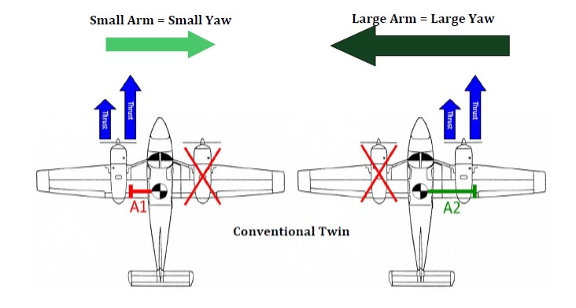
\includegraphics[width=0.9\linewidth]{pfactor}
\end{center}

\subsubsection{Accelerated Slipstream}

The loss of induced airflow created by the propeller over the dead engine wing results in a
loss of lift on that wing. This loss of lift causes a roll towards the dead engine and will
require additional aileron deflection into the operating engine. Due to P-factor, the
accelerated slipstream of the right engine has a longer moment-arm (A2) than the left
engine (A1) because the descending (greater-thrust) propeller blade is outboard.

\begin{center}
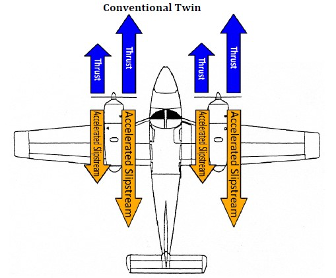
\includegraphics[width=0.5\linewidth]{accel1}
\end{center}

\begin{center}
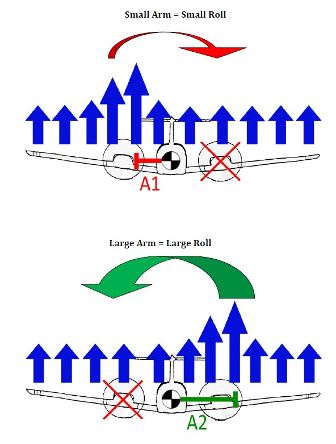
\includegraphics[width=0.5\linewidth]{accel2}
\end{center}

\subsubsection{Spiraling Slipstream}

Both engines produce spiraling slipstreams, but the left engine’s spiraling slipstream is directed towards the rudder, making it more effective. The right engine’s spiraling slipstream is directed away from the rudder. In the event of
left engine failure, the rudder becomes less effective due to the loss of the critical engine’s spiraling slipstream.
Therefore, with critical engine failure maintaining directional control requires more rudder authority.

\begin{center}
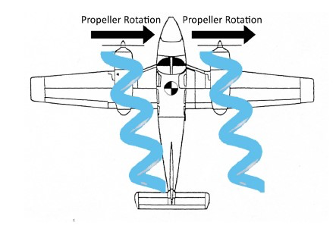
\includegraphics[width=0.5\linewidth]{spiraling}
\end{center}

\subsubsection{Torque}

Torque is the opposite reaction to the clockwise turning of the propellers. Both engines produce a rolling tendency
to the left. With the right engine operating (critical engine inoperative), torque adds to the yaw/roll produced by
asymmetric thrust. With the left engine operating, torque counteracts the yaw/roll produced by asymmetric thrust.

\begin{center}
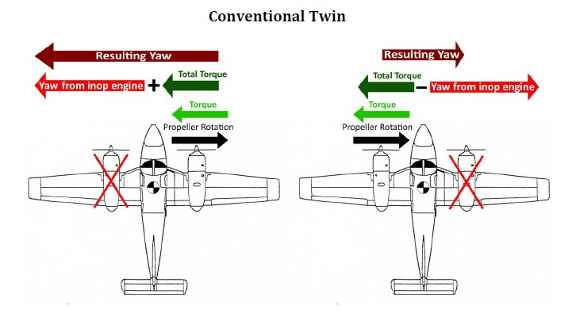
\includegraphics[width=0.9\linewidth]{torque}
\end{center}

\subsection{$V_{MC}$}

\vmc is defined as the minimum speed at which you can maintain directional control
with ithe sudden loss of the critical engine. The actual speed at which you will
lose directional control will vary depending on conditions on a
given day. The \emph{published \vmc airspeed} is dictated by a set of conditions in
14 CFR (FAR) 23.149. \vmc is marked with a \textbf{\textcolor{red}{red line}} on the airspeed indicator.
For the Duchess, this airspeed is \textcolor{red}{65 KIAS}.

On August 30, 2017, a substantial rewrite of 14 CFR (FAR) 23 went into effect. This
rewrite eliminated 23.149 from the current regulations. However, it remains the
certification basis for many of the light piston twin airplanes we fly today. For
light twins certificated under the new Part 23, such as the Tecnam P2006, we would
see similar requirements under 14 CFR (FAR) 23.2xxx. Since this document focuses on
the Duchess, we restrict our discussion to the ``old'' 14 CFR (FAR) 23, which is
archived on ecfr.gov.

\subsection{Determination of $V_{MC}$}

Under the ``old'' 14 CFR Part 23, manufactures of multiengine aircraft were required to demonstrate and publish a \vmc
(minimum control airspeed) under the following specific conditions, which are either set for Standardization (S), or are the Worst Case (W):

\vbox{%
\begin{enumerate}
    \item \textbf{Standard Day} (S) (15\degree C and 29.92" at sea level)
    \item \textbf{Maximum sea level takeoff weight} (S)
    \item \textbf{The most rearward allowable center of gravity} (W)
    \item \textbf{The critical engine failed} (W) and the propeller is
        \begin{enumerate}
            \item Windmilling, or
            \item Feathered, if the aircraft has an auto feather system (rare in light twins)
        \end{enumerate}
    \item \textbf{Takeoff at maximum available power on the good engine} (W)
    \item \textbf{Landing gear up} (W)
    \item \textbf{Flaps in the takeoff position} (S)
    \item \textbf{No more than 5\degree{} of bank into the good engine} (S)
\end{enumerate}}

A further factor is the pilot ability, Part 23 states that recovery from loss of directional
control at \vmc should not require more than average pilot technique and the recovery should
be accomplished within 20\degree{} of original heading.

Apart from the 5\degree{} bank, max gross weight, standard day, and flaps, the remaining factors
are all worst case, and they lead to the highest \vmc to be published by the manufacturer
(65 KIAS for the Duchess), or are related to the takeoff scenario.

When considering \vmc, realize that lower \vmc is better. Anything that lowers \vmc
will increase controllability at lower airspeed, giving more margin for error in
single-engine operation.

\subsubsection{Conditions that the FAA Requires for Published \vmc (14 CFR 23.149)}

What follows is a list of conditions required to be met by manufacturers in
determining the published \vmc value for certification. Understanding the
regulatory criteria is important for understanding how existing conditions and
aircraft control influence single-engine controllability.

The conditions required for certification represent the worst-case scenario
for controllability: an engine failure shortly after takeoff, with the
aircraft in the climb-out configuration. However, not every condition required for
certification is necessarily worst-case (W); some conditions are specified primarily
for standardization purposes (S).

\subsubsection{Standard conditions (ISA: 15\degree C and 29.92” Hg) (Standardization)}

\vmc decreases with increase density altitude. Any condition that decreases
power on the operating engine such as increased altitude, low air density or
high temperature will in turn mean less thrust, which creates less yaw, so \vmc
will decrease. The opposite is also true for any condition that increases power,
such as lower altitude, high density or low temperature, which will increase \vmc.

\emph{Memory aid: Hot = Good}

\subsubsection{Maximum sea-level power on operating engine (Worst case)}

Maximum power on the good engine increases \vmc due to increased asymmetric thrust.

\subsubsection{Critical engine windmilling or auto-feathered if installed (Worst case)}

The windmilling propeller creates drag, which is asymmetric. Therefore, more rudder
authority will be required to offset this asymmetric drag. \vmc is higher
with a windmilling propeller on the inoperative engine.

\subsubsection{Landing gear retracted (Worst case)}

The gear and gear doors extended tend to act like keels on a boat and resist rolling and yawing tendencies by
shifting the center of gravity down the vertical axis of the airplane. Additionally, on a tricycle-gear airplane, the
main gear are located aft of the center of gravity and produce \emph{stabilizing drag} when extended, like a drag chute
would. \vmc is \emph{lower with gear down}.

\subsubsection{Flaps in the takeoff configuration (Standardization)}

A number of considerations determine the relationship between flap setting and \vmc. With flaps extended a lesser
angle of attack is necessary to produce the same amount of lift. Therefore, P-factor is less as well as yaw.
Additionally, flaps increase drag aft of the C.G., providing a stabilizing effect. However, deploying flaps creates
additional lift on the wing with the operating engine since lift increases with the same airspeed. Therefore it is not
straightforward to say that \vmc changes one way or the other with flaps deployed, and this relationship may vary
depending on the airplane.

The Duchess procedures call for flaps fully retracted for takeoff.

\subsubsection{Maximum 5\degree{} bank into good engine (Standardization)}

The maximum bank allowed by the regulations for \vmc determination is five degrees. Any sideslip toward the good
engine increases controllability due to increased rudder effectiveness – the sideslip results in weathervaning
tendencies toward the operating engine. Likewise, sideslip toward the inoperative engine decreases controllability
by introducing a weathervaning moment away from the operating engine. Specifying a maximum of five degrees
limits the manufacturers to a realistic bank angle.

It should be remembered that a bank angle of three degrees towards the good engine with the ball 1/2 off-center
results in minimum drag and maximum climb. Five degrees of bank towards the good engine actually results in a
sideslip toward the good engine, increasing drag but increasing controllability.

\subsubsection{Maximum gross weight (Standardization)}

\vmc is determined at max gross weight. Primarily this is a reference point for standardization purposes.

When the airplane is banked, a sideslip occurs because a component of weight is acting along the wing (similar to
the idea of a wing-down crosswind approach). The spanwise component of weight and sideslip is greater at a higher
weight than a lower weight. Because of this, when the airplane is banked into the operative engine beyond the
zero-sideslip angle, \vmc increases with the decrease in weight, and vice versa.

\emph{Memory aid: Weight increases side slip effectiveness and lowers \vmc.}

\subsubsection{Most adverse CG (usually aft legal CG limit) (Worst case)}

As the CG moves aft, the moment arm between the rudder and C.G. is shortened, producing less leverage for the
rudder. The further aft the C.G., the more rudder authority is required to offset the asymmetric thrust, requiring
greater airspeed. \vmc is higher with an aft C.G.

\subsubsection{Ground effect negligible (Worst case)}

In ground effect there is a reduction in induced drag, so if an engine failure should occur while in ground effect a
lower than normal angle of attack would be required to create the same amount of lift as when out of ground effect.
A lower angle of attack would decrease the effect of P-factor, reduce yaw, and lower \vmc. Operating out of ground
effect results in a higher \vmc than in ground effect.

\begin{center}
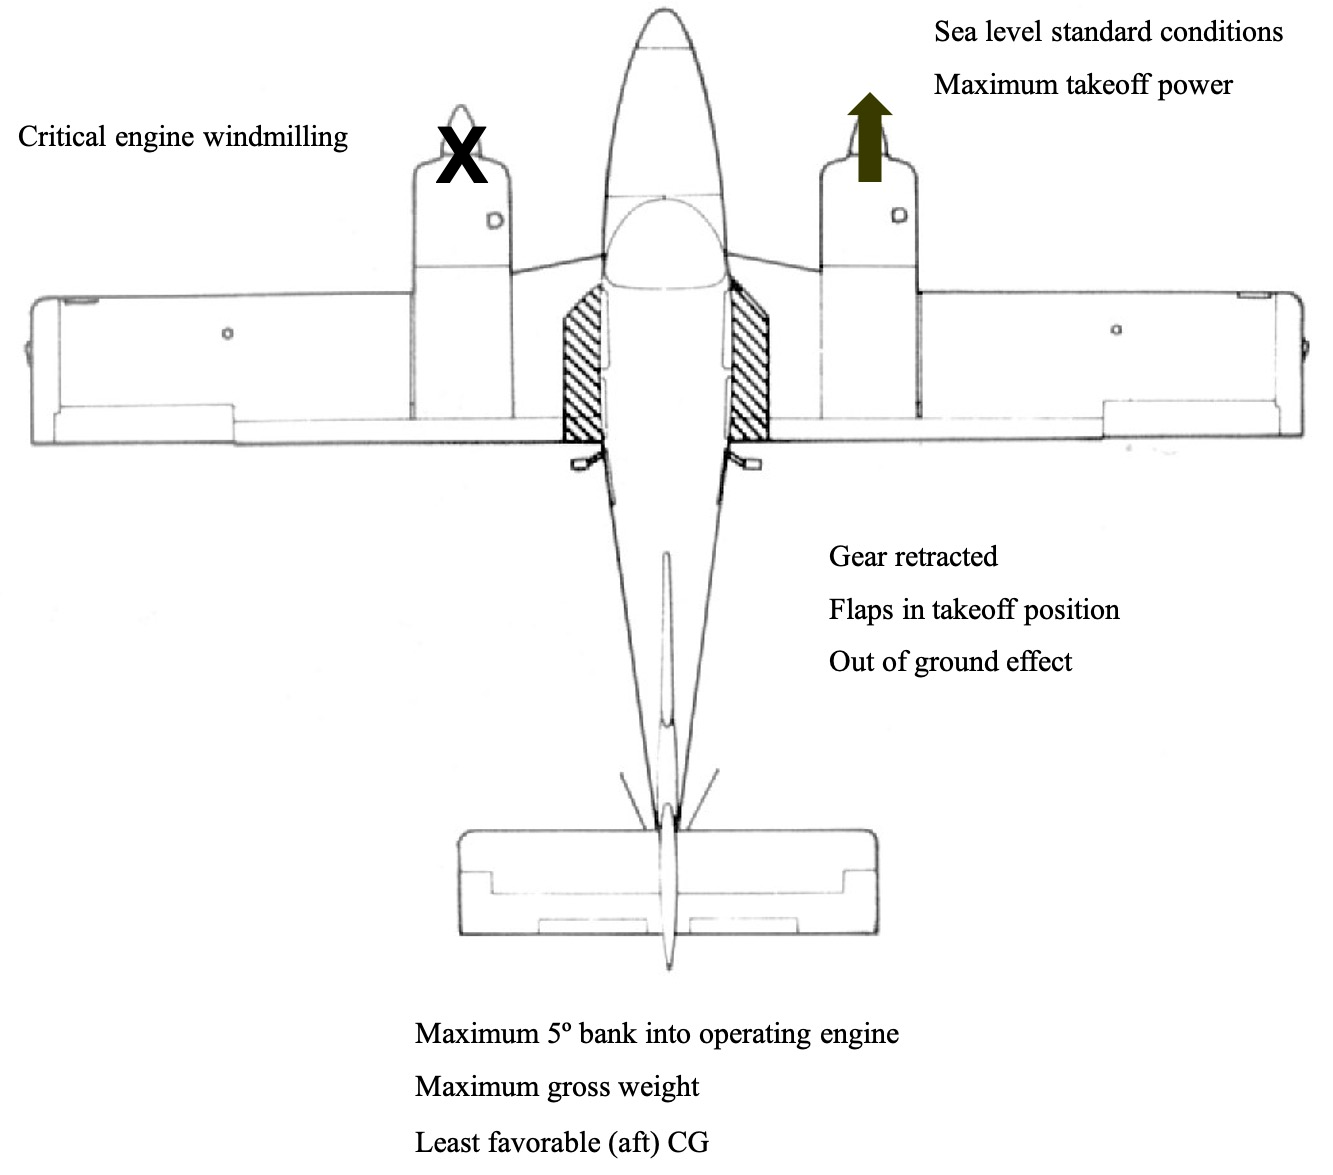
\includegraphics[width=0.9\linewidth]{vmc-conditions}
\end{center}

\emph{Memory aid: Any increase in yaw or decrease in rudder authority \textbf{increases} \vmc!}

\emph{Memory aid: In the least favorable (aft) CG, the arm to the rudder is reduced, so the rudder is less effective.}

\section{Altitude vs. $V_{MC}$ and Stall Speed}

As density altitude increases, \vmc will decrease due to less power output from the operating engine (you'll lose
directional control at a slower airspeed). Indicated stall speed remains relatively constant for all density altitudes.
Thus, it is easily possible for \vmc to be lower than stall speed. When this happens a possible spin could develop
during \vmc demonstrations or during other single-engine operation, real or simulated.

If loss of directional control occurs during single-engine operation, \textbf{IMMEDIATELY} reduce power on the good
engine and lower the nose to regain airspeed.

\begin{center}
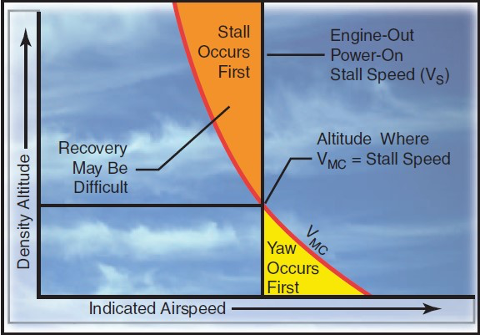
\includegraphics[width=0.8\linewidth]{vmc-stall}
\end{center}

\section{The Zero-Sideslip Condition}

As previously stated, a twin with only one engine operating must counteract the yaw and roll produced by
asymmetric thrust with rudder and aileron. The asymmetric thrust and the \textbf{horizontal lift} produced by the rudder
result in a net sideslip toward the \textbf{inoperative} engine when the wings of the airplane are held level,
causing a turn \emph{away} from the operating engine. This sideslip increases drag and degrades performance
just as a sideslip would in a single.

To overcome this sideslip, the airplane must be banked into the operative engine. The sideslip caused by the bank
angle and ball half-centered cancels out the sideslip created by the engine and rudder resulting in a
\textbf{zero-sideslip condition}. The zero-sideslip condition reduces
drag and therefore improves climb performance (or minimizes rate
of descent). In the Duchess, the bank angle that results in zero sideslip is approximately three degrees.

\begin{center}
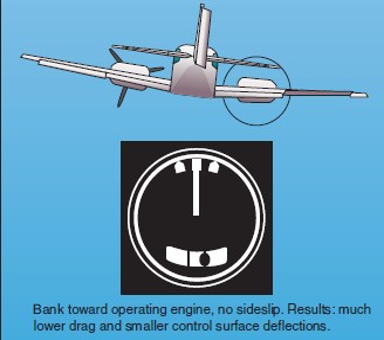
\includegraphics[width=0.6\linewidth]{zero-sideslip}
\end{center}

\emph{Memory aid: Heavier means good engine is less effective, which reduces \vmc.}

\emph{Memory aid: Tail induces centripetal force which turns the airplane. So, you have to counteract that turn
with a bank angle of \emph{3\degree}}.

\chapter{Limitations}

\section{Duchess Speeds}


\begin{table}[h]
\centering
\begin{tabular}{lll}
\textcolor{red}{\textbf{$V_{MC}$}}      & \textbf{65}      & Minimum control speed.                                           \\
\textbf{$V_{S0}$}                       & \textbf{60}      & Stall: landing configuration.                                    \\
\textbf{$V_{S1}$}                       & \textbf{70}      & Stall: clean configuration.                                      \\
\textbf{$V_{XSE}$}                      & \textbf{85}      & Best rate of climb, one engine.                                  \\
\textcolor{blue}{\textbf{$V_{YSE}$}}    & \textbf{85}      & Best angle of climb, one engine.                                 \\ \hline
\multicolumn{1}{|l}{\textbf{$V_{SSE}$}} & \textbf{71}      & \multicolumn{1}{l|}{Intentional one engine inoperative speed.}   \\ \hline
\textbf{$V_A$}                          & \textbf{132}     & Maneuvering speed (at Max gross weight).                         \\
\textbf{$V_{LO}$}                       & \textbf{140/112} & Landing gear operating extend/retract.                           \\
\textbf{$V_{LE}$}                       & \textbf{140}     & Max landing gear extended.                                       \\
\textbf{$V_{FE}$}                       & \textbf{120/110} & Max flaps extended 20/35.                                        \\
\textbf{$V_{NO}$}                       & \textbf{154}     & Max structural cruising speed.                                   \\
\textbf{$V_{NE}$}                       & \textbf{194}     & Never exceed speed.                                              \\
\textbf{$V_R$}                          & \textbf{71}      & Rotation speed. For training purposes, $V_R$ is increased to 80. \\
\textbf{$V_X$}                          & \textbf{71}      & Best angle of climb.                                             \\
\textbf{$V_Y$}                          & \textbf{85}      & Best rate of climb.                                              \\
\textbf{}                               & \textbf{140}     & Emergency descent. \emph{Do not exceed!}                         \\
\textbf{}                               & \textbf{100}     & Emergency landing gear extension (free fall), maximum.           \\
\textbf{}                               & \textbf{95}      & Best glide: 12:1 with propellers feathered.                      \\
\textbf{}                               & \textbf{25}      & Maximum demonstrated crosswind component.
\end{tabular}
\end{table}

\section{Weight Limits}

\begin{table}[h]
\centering
\begin{tabular}{ll}
\textbf{Maximum Ramp Weight}              & 3916 Pounds \\
\textbf{Maximum Takeoff Weight}           & 3900 Pounds \\
\textbf{Maximum Landing Weight}           & 3900 Pounds \\
\textbf{Maximum Zero Fuel Weight}         & 3500 Pounds \\
\textbf{Maximum Baggage Compartment Load} & 200 Pounds 
\end{tabular}
\end{table}

\chapter{Emergency Procedures}

\textbf{KNOW PROCEDURES BY MEMORY!}

\section{Engine Failure in Flight (above 3000' AGL)}

\subsection{Procedures}

\textbf{Maintain directional control!}

\textbf{ALL AVAILABLE POWER:}
\begin{enumerate}
    \item \textbf{PITCH FOR \textcolor{blue}{BLUE LINE} - \vyse (85 KIAS),\\OR maintain altitude at a higher airspeed if able.}
    \item \textbf{\textcolor{red}{MIXTURES} SET (max available power)}
    \item \textbf{\textcolor{blue}{PROPELLERS} Full Forward}
    \item \textbf{THROTTLES Full Power}
\end{enumerate}

\textbf{CLEAN UP:}
\begin{enumerate}
    \item \textbf{FLAPS UP (or as required)}
    \item \textbf{GEAR UP (or as required)}
    \item \textbf{Trim and bank into good engine.}
\end{enumerate}

\textbf{IDENTIFY/VERIFY:}
\begin{enumerate}
    \item \textbf{IDENTIFY Dead foot = dead engine.}
    \item \textbf{VERIFY Power idle on dead engine. No change in performance - verified.}
\end{enumerate}

\textbf{FIX OR FEATHER:}
\begin{itemize}
    \item \textbf{DECISION Based upon situation/altitude (Restart or Feather?)}
\end{itemize}

Rarely do engines fail suddenly and completely (fuel starvation is the exception). If an engine is running poorly, but
developing some power, \textbf{you are better off letting it run} (above 3000 AGL) until you sort out the problem. The
decision to feather should be made with some deliberation. A catastrophic engine failure would require feathering
the engine (avoiding a potential fire), however, a rough running engine should not be feathered as any horsepower it
is producing potentially helps.

\textbf{The exception is during a critical phase of flight}, such as initial climb-out,
approach or landing. During these phases of flight the propeller on the problem engine should be feathered
immediately, as there is not enough time to safely perform the fix procedures. Maintaining aircraft control is
\emph{the priority} and you should land as soon and as safely as possible.

\textbf{FIX:}

\textbf{CHECK (\textcolor{red}{Red Items}) - only on affected engine.}
\begin{enumerate}
    \item \textbf{Fuel - ON}
    \item \textbf{Carburetor Heat - ON}
    \item \textbf{Mixture - SET (max available power)}
    \item \textbf{Boost Pumps - ON}
    \item \textbf{Magnetos - CYCLE Left - Right - Both}
\end{enumerate}

\textbf{\textcolor{red}{WARNING} Feathering the wrong engine is incredibly dangerous!
Work methodically to make certain the correct engine is feathered.}

\textbf{FEATHER:}
\begin{enumerate}
    \item \textbf{Feather Propeller on inoperative engine.}
    \item \textbf{Power as needed on good engine to maintain altitude/airspeed.\\Minimum speed: \textcolor{blue}{BLUE LINE 85 KIAS}.}
\end{enumerate}

\emph{Memory aid: 3\degree{} bank for slip.}

\textbf{SHUTDOWN AND SECURE ENGINE:}
\begin{itemize}
    \item \textbf{Mixture - Idle Cutoff}
    \item \textbf{Fuel Selector - OFF}
    \item \textbf{Cowl Flaps - Open on operative engine, closed on inoperative engine.}
    \item \textbf{Fuel Pump - OFF}
    \item \textbf{Magnetos - OFF}
    \item \textbf{Alternator Switch - OFF}
    \item \textbf{Notify ATC.}
    \item \textbf{Land as soon as practical.}
\end{itemize}

\textbf{\textcolor{red}{** NOW REFER TO CHECKLIST. **}}


\section{Engine Failure During or After Takeoff}

\subsection{Procedures}

{\centering
\textbf{DURING INITIAL CLIMB OUT THE NOSE NEEDS TO BE LOWERED\\
5 DEGREES OR MORE TO MAINTAIN 85 KIAS!!!}
\par }

Bank approximately \textbf{3 degrees} toward the good engine with the rudder ball half out toward the good engine. This
will provide maximum climb performance. \textbf{Each degree of bank back toward the inoperative engine increases \vmc
by 3 knots per degree. Therefore, with only a 2 degree bank toward the operative engine, \vmc might be 3 knots higher
than published.}

If the pilot inadvertently or instinctively tries to hold wings level in an engine out situation, \vmc
\textbf{CAN INCREASE AS MUCH AS 15 KNOTS. THE AIRCRAFT COULD BE UNCONTROLLABLE AT A
SPEED AS HIGH AS \vyse!} This situation \textbf{WILL EXIST} if the pilot flies wings level and tries to maintain heading
with the ball centered.

\emph{Memory aid: Raise the dead (engine).}

\subsection{Power-Loss Briefing (Before Takeoff)}

A power loss briefing is to be given before takeoff to remind the pilot of the actions to be taken in the event of a
power loss during or after the takeoff roll. Time is critical so actions must be immediate but deliberate.

\bfseries{

Loss of directional control on the ground:
\begin{itemize}
    \item Throttles - IDLE
    \item Regain Control (mostly rudder)
    \item Brake straight ahead
\end{itemize}

Airborne loss of directional control: usable runway remaining and gear down:
\begin{itemize}
    \item Throttles – IDLE
    \item Land
    \item Brake straight ahead
\end{itemize}

Airborne loss of directional control: no usable runway remaining or gear up:
\begin{itemize}
    \item All available power (maintain Heading and Blue Line):
    \item Clean Up
        \begin{itemize}
            \item[\ding{226}] Flaps – UP
            \item[\ding{226}] Gear – UP
        \end{itemize}
    \item Identify dead engine
    \item Verify dead engine
    \item Feather dead engine
    \item Return for landing
\end{itemize}
%} % \bfseries
\mdseries

\section{Airman Certification Standards}

\emph{Source: FAA-S-ACS-7B, Commercial Pilot for Airplane Category Airman Certification Standards, November 2023} 

\subsection{X.A Maneuvering with One Engine Inoperative (AMEL, AMES)}

% From https://www.tablesgenerator.com/ with modifications for [H] and raggedleft/right.

\begin{table}[H]
\centering
\begin{tabular}%
  {>{\raggedleft\arraybackslash}p{0.15\linewidth}%
   >{\raggedright\arraybackslash}p{0.8\linewidth}%
  }
%\textbf{Task}                                                      & \textbf{A. Maneuvering with One Engine Inoperative (AMEL, AMES)}                                                                                                        \\ \hline
\textit{References:}                                                & \textit{FAA-H-8083-2, FAA-H-8083-3, FAA-H-8083-25; FAA-P-8740-66; POH/AFM}                                                                                              \\
\textbf{Objective:}                                                 & To determine the applicant exhibits satisfactory knowledge, risk management, and skills associated with maneuvering with one engine inoperative.                        \\
\textit{\textbf{Note:}}                                             & \textit{See Appendix 2: Safety of Flight and Appendix 3: Aircraft, Equipment, and Operational Requirements \& Limitations for information related to this Task.}        \\ \hline
\textbf{Knowledge:}                                                 & The applicant demonstrates understanding of:                                                                                                                            \\
\textit{CA.X.A.K1}                                                 & Factors affecting minimum controllable speed (VMC)                                                                                                                      \\
\textit{CA.X.A.K2}                                                 & VMC (red line) and best single-engine rate of climb airspeed (VYSE) (blue line).                                                                                        \\
\textit{CA.X.A.K3}                                                 & How to identify, verify, feather, and secure an inoperative engine.                                                                                                     \\
\textit{CA.X.A.K4}                                                 & Importance of drag reduction, including propeller feathering, gear and flap retraction, the manufacturer's recommended control input and its relation to zero sideslip. \\
\textit{CA.X.A.K5}                                                 & Feathering, securing, unfeathering, and restarting.                                                                                                                     \\ \hline
\textbf{\begin{tabular}[c]{@{}l@{}}Risk\\ Management:\end{tabular}} & The applicant is able to identify, assess, and mitigate risk associated with:                                                                                           \\
\textit{CA.X.A.R1}                                                 & Potential engine failure during flight.                                                                                                                                 \\
\textit{CA.X.A.R2}                                                 & Collision hazards.                                                                                                                                                      \\
\textit{CA.X.A.R3}                                                 & Configuring the airplane.                                                                                                                                               \\
\textit{CA.X.A.R4}                                                 & Low altitude maneuvering, including stall, spin, or controlled flight into terrain (CFIT).                                                                              \\
\textit{CA.X.A.R5}                                                 & Distractions, task prioritization, loss of situational awareness, or disorientation.                                                                                    \\ \hline
\textbf{Skills:}                                                    & The applicant exhibits the skill to:                                                                                                                                    \\
    \textit{CA.X.A.S1}                                                          & Recognize an engine failure, maintain control, use manufacturer’s memory item procedures, and use appropriate emergency procedures.                                     \\
    \textit{CA.X.A.S2}                                                          & Set the engine controls, identify and verify the inoperative engine, and feather the appropriate propeller.                                                             \\
    \textit{CA.X.A.S3}                                                          & Use flight controls in the proper combination as recommended by the manufacturer, or as required to maintain best performance, and trim as required.                    \\
    \textit{CA.X.A.S4}                                                          & Attempt to determine and resolve the reason for the engine failure.                                                                                                     \\
    \textit{CA.X.A.S5}                                                          & Secure the inoperative engine and monitor the operating engine and make necessary adjustments.                                                                          \\
    \textit{CA.X.A.S6}                                                          & Restart the inoperative engine using manufacturer’s restart procedures.                                                                                                 \\
    \textit{CA.X.A.S7}                                                          & Maintain altitude ±100 feet or minimum sink rate if applicable, airspeed ±10 knots, and selected headings ±10°.                                                         \\
    \textit{CA.X.A.S8}                                                          & Complete the appropriate checklist(s).                                                                                                                                 
\end{tabular}
\end{table}
  
% Engine Failure During Takeoff Before VMC (Simulated) (AMEL, AMES)

\newpage

\subsection{IX.E Engine Failure During Takeoff Before VMC (Simulated) (AMEL, AMES)}

\begin{table}[h]
\centering
\begin{tabular}%
  {>{\raggedleft\arraybackslash}p{0.15\linewidth}%
   >{\raggedright\arraybackslash}p{0.8\linewidth}%
  }
\textit{References:}       & \textit{FAA-H-8083-2, FAA-H-8083-3, FAA-H-8083-25; FAA-P-8740-66; POH/AFM}                                                                                                        \\
\textbf{Objective:}        & To determine the applicant exhibits satisfactory knowledge, risk management, and skills associated with engine failure during takeoff before minimum controllable airspeed (VMC). \\
\textit{\textbf{Note:}}    & \textit{See Appendix 2: Safety of Flight and Appendix 3: Aircraft, Equipment, and Operational Requirements \& Limitations for information related to this Task.}                  \\ \hline
\textbf{Knowledge:}        & The applicant demonstrates understanding of:                                                                                                                                      \\
\textit{CA.IX.E.K1}        & Factors affecting minimum controllable speed (VMC).                                                                                                                               \\
\textit{CA.IX.E.K2}        & VMC (red line) and best single-engine rate of climb airspeed (VYSE) (blue line).                                                                                                  \\
\textit{CA.IX.E.K3}        & Accelerate/stop distance.                                                                                                                                                         \\ \hline
\textbf{\begin{tabular}[c]{@{}l@{}}Risk\\ Management:\end{tabular}}  & The applicant is able to identify, assess, and mitigate risk associated with:                                                                                                     \\
\textit{CA.IX.E.R1}        & Potential engine failure during takeoff.                                                                                                                                          \\
\textit{CA.IX.E.R2}        & Configuring the airplane.                                                                                                                                                         \\
\textit{CA.IX.E.R3}        & Distractions, task prioritization, loss of situational awareness, or disorientation.                                                                                              \\ \hline
\textbf{Skills:}           & The applicant exhibits the skill to:                                                                                                                                              \\
\textit{CA.IX.E.S1}        & Close the throttles smoothly and promptly when a simulated engine failure occurs.                                                                                                 \\
\textit{CA.IX.E.S2}        & Maintain directional control and apply brakes (AMEL), or flight controls (AMES), as necessary.                                                                                   
\end{tabular}
\end{table}

\newpage

\subsection{IX.F Engine Failure After Liftoff (Simulated) (AMEL, AMES)}

\begin{table}[H]
\centering
%\begin{tabular}{rl}
\begin{tabular}%
  {>{\raggedleft\arraybackslash}p{0.15\linewidth}%
   >{\raggedright\arraybackslash}p{0.8\linewidth}%
  }
\textit{References:}                                                                    & \textit{FAA-H-8083-2, FAA-H-8083-3, FAA-H-8083-25; FAA-P-8740-66; POH/AFM}                                                                                                                                                 \\
\textbf{Objective:}                                                                     & To determine the applicant exhibits satisfactory knowledge, risk management, and skills associated with engine failure after liftoff.                                                                                      \\
\textit{\textbf{Note:}}                                                                 & \textit{See Appendix 2: Safety of Flight and Appendix 3: Aircraft, Equipment, and Operational Requirements \& Limitations for information related to this Task.}                                                           \\ \hline
\textbf{Knowledge:}                                                                     & The applicant demonstrates understanding of:                                                                                                                                                                               \\
\textit{CA.IX.F.K1}                                                                     & Factors affecting minimum controllable speed (VMC).                                                                                                                                                                        \\
\textit{CA.IX.F.K2}                                                                     & VMC (red line), VYSE (blue line), and safe single-engine speed (VSSE).                                                                                                                                                     \\
\textit{CA.IX.F.K3}                                                                     & Accelerate/stop and accelerate/go distances.                                                                                                                                                                               \\
\textit{CA.IX.F.K4}                                                                     & How to identify, verify, feather, and secure an inoperative engine.                                                                                                                                                        \\
\textit{CA.IX.F.K5}                                                                     & Importance of drag reduction, including propeller feathering, gear and flap retraction, the manufacturer’s recommended control input and its relation to zero sideslip.                                                    \\
\textit{CA.IX.F.K6}                                                                     & Simulated propeller feathering and the evaluator’s zero-thrust procedures and responsibilities.                                                                                                                            \\ \hline
\multicolumn{1}{l}{\textbf{\begin{tabular}[c]{@{}l@{}}Risk\\ Management:\end{tabular}}} & The applicant is able to identify, assess, and mitigate risk associated with:                                                                                                                                              \\
\textit{CA.IX.F.R1}                                                                     & Potential engine failure after lift-off.                                                                                                                                                                                   \\
\textit{CA.IX.F.R2}                                                                     & Collision hazards.                                                                                                                                                                                                         \\
\textit{CA.IX.F.R3}                                                                     & Configuring the airplane.                                                                                                                                                                                                  \\
\textit{CA.IX.F.R4}                                                                     & Low altitude maneuvering, including stall, spin, or controlled flight into terrain (CFIT).                                                                                                                                 \\
\textit{CA.IX.F.R5}                                                                     & Distractions, task prioritization, loss of situational awareness, or disorientation.                                                                                                                                       \\ \hline
\textbf{Skills:}                                                                        & The applicant exhibits the skill to:                                                                                                                                                                                       \\
\textit{CA.IX.F.S1}                                                                     & Promptly recognize an engine failure, maintain control, and use appropriate emergency procedures.                                                                                                                          \\
\textit{CA.IX.F.S2}                                                                     & Establish VYSE; if obstructions are present, establish best single-engine angle of climb speed (VXSE) or VMC +5 knots, whichever is greater, until obstructions are cleared. Then transition to VYSE.                      \\
\textit{CA.IX.F.S3}                                                                     & Reduce drag by retracting landing gear and flaps in accordance with the manufacturer’s guidance.                                                                                                                           \\
\textit{CA.IX.F.S4}                                                                     & Simulate feathering the propeller on the inoperative engine (evaluator should then establish zero thrust on the inoperative engine).                                                                                       \\
\textit{CA.IX.F.S5}                                                                     & Use flight controls in the proper combination as recommended by the manufacturer, or as required to maintain best performance, and trim as required.                                                                       \\
\textit{CA.IX.F.S6}                                                                     & Monitor the operating engine and aircraft systems and make adjustments as necessary.                                                                                                                                       \\
\textit{CA.IX.F.S7}                                                                     & Recognize the airplane’s performance capabilities. If a climb is not possible at VYSE, maintain VYSE and return to the departure airport for landing, or initiate an approach to the most suitable landing area available. \\
\textit{CA.IX.F.S8}                                                                     & Simulate securing the inoperative engine.                                                                                                                                                                                  \\
\textit{CA.IX.F.S9}                                                                     & Maintain heading ±10° and airspeed ±5 knots.                                                                                                                                                                               \\
\textit{CA.IX.F.S10}                                                                    & Complete the appropriate checklist(s).
\end{tabular}
\end{table}

\chapter{Normal Procedures}

Refer to aircraft checklists for detailed procedures. The procedures listed below
should be memorized and chair-flown until familiar.

% vim :set indentexpr=

\section{Takeoff}

\begin{itemize}[label={}]
\item Takeoff briefing – GIVEN (see Emergency Procedures)
\item Taxi into position on the runway for takeoff
\item Brakes – APPLY AND HOLD
\item Throttles – 20 MP
\item Engine Gauges – CHECK IN THE GREEN
\item Brakes – RELEASE
\item Throttles – FULL
\item Airspeed Indicator – CHECK ALIVE
\item Rotate at 80 KIAS
\item Gear Up (when positive rate of climb)
\item Climb at 90 KIAS
\end{itemize}

\section{Climb}
\textbf{At 500' AGL:}
\begin{itemize}[label={}]
\item Throttles – 25” MP
\item Propellers – 2500 RPM
\item Cruise climb at 100 KIAS
\item Turn Crosswind or Depart, as Required
\end{itemize}
\textbf{If staying in the pattern, at pattern altitude:}
\begin{itemize}[label={}]
\item Throttles – 20” MP
\item Propellers – 2400 RPM
\end{itemize}

\section{Approach to Landing}
\textbf{Before reaching midfield:}
\begin{itemize}[label={}]
\item Power – 20” MP / 2400 RPM or as required for 100 KIAS
\item Gas: Fuel Selectors – ON; Aux Pumps – ON
\item Undercarriage – DOWN BELOW 140 KIAS
\item Mixtures – SET (max available power)
\item Propellers – 2400 UNTIL FINAL
\item Cowl Flaps – CLOSED
\item Seat Belts – FASTENED
\end{itemize}

\textbf{Abeam the numbers:}
\begin{itemize}[label={}]
\item Throttles – 15” MP
\item Flaps – ID, VERIFY, 10 DEGREES (3 SEC.)
\item Pitch – HALF GROUND / HALF SKY
\item Airspeed – 100 KIAS
\end{itemize}

\textbf{Base leg:}
\begin{itemize}[label={}]
\item Gear Indicators – 3 GREEN
\item Flaps – ID, VERIFY, 20 DEGREES (2 SEC.)
\item Airspeed – 95 KIAS
\item Power – AS REQUIRED
\end{itemize}

\textbf{On final approach (left-to-right flow check):}
\begin{itemize}[label={}]
\item Gear Indicators – 3 GREEN
\item Propellers – FULL FORWARD
\item Mixtures – FULL FORWARD
\item Flaps – FULL (DN)
\item Windsock – CHECK
\item Airspeed – 85 UNTIL SHORT FINAL
\end{itemize}

\textbf{Over the threshold –} CONFIRM 3 GREEN

\section{Touch and Go}

\textbf{Touch and go landings are to be performed only with a Pilot’s Choice Instructor!}

\textbf{On the runway:}
\begin{itemize}[label={}]
\item Flaps – IDENTIFIED (wait for instructor to call VERIFIED) and RETRACTED
\item Cowl Flaps – OPENED
\item Throttles – ADVANCE FOR TAKEOFF \emph{All Available Power}
\end{itemize}

\section{Go-Around}


\begin{itemize}[label={}]
\item \textbf{CRAM} Power - FULL \emph{All Available Power}
\item \textbf{CLIMB} Climb at 85 KIAS (\vyse)
\item \textbf{CLEAN} Flaps – RETRACT ABOVE 71 KIAS
\item \textbf{............} Landing Gear – RETRACT AT 85 AND POSITIVE RATE OF CLIMB
\item \textbf{COOL} Cowl Flaps - OPEN
\item \textbf{CALL} Intentions - ANNOUNCE
\end{itemize}

\newpage

\section{VFR Approach Airspeeds and Power Settings}

\subsection{Traffic Pattern}


% Please add the following required packages to your document preamble:
% \usepackage[normalem]{ulem}
% \useunder{\uline}{\ul}{}
\begin{table}[H]
\begin{tabular}{llll}
              & {\ul Airspeed} & {\ul MP/RPM}             & {\ul Flaps/Configuration}      \\
DOWNWIND      & \textbf{110}   & \textbf{20”/2400}        & \textbf{0}                     \\
Abeam NUMBERS & \textbf{100}   & \textbf{15”/2400}        & \textbf{10\degree{} (3 seconds)}       \\
BASE          & \textbf{100}   & \textbf{15”/2400}        & \textbf{20\degree{} (2 seconds)}       \\
FINAL         & \textbf{90}    & \textbf{12-15”/High RPM} & \textbf{Full flaps (optional)} \\
Over NUMBERS  & \textbf{85}    & \textbf{12-15”/High RPM} & \textbf{Full flaps (optional)}
\end{tabular}
\end{table}


\subsection{Take Off and Climb Out}

% Please add the following required packages to your document preamble:
% \usepackage[normalem]{ulem}
% \useunder{\uline}{\ul}{}
\begin{table}[H]
\begin{tabular}{llll}
         & {\ul Airspeed}              & {\ul MP/RPM}          & {\ul Flaps/Configuration}                       \\
ROTATION & \textbf{80}                 & \textbf{Max/High RPM} & \textbf{0}                                      \\
CLIMB    & \textbf{90 (\vyse or faster)} & \textbf{25”/2500}     & \textbf{0 / Gear up:}     \\
         &                             &                       & \textbf{positive rate, no runway.}
\end{tabular}
\end{table}

\subsection{\textcolor{red}{Single-Engine Pattern}}

% Please add the following required packages to your document preamble:
% \usepackage[normalem]{ulem}
% \useunder{\uline}{\ul}{}
\begin{table}[H]
\begin{tabular}{llll}
         & {\ul Airspeed} & {\ul MP/RPM}              & {\ul Flaps/Configuration}   \\
DOWNWIND & \textbf{\textcolor{blue}{85+}}   & \textbf{As Required/2600} & \textbf{None.}              \\
NUMBERS  & \textbf{\textcolor{blue}{85+}}   & \textbf{20”/2600}         & \textbf{As Required.}       \\
BASE     & \textbf{\textcolor{blue}{85+}}   & \textbf{17-20”/2600}      & \textbf{As Required.}       \\
FINAL    & \textbf{\textcolor{blue}{85}}    & \textbf{Reduce/2600}      & \textbf{20º (for training)}
\end{tabular}
\end{table}

{\centering
\textbf{\textcolor{red}{*GEAR \& FLAPS DOWN \underline{ONLY} WHEN LANDING IS ASSURED!}}
\par }


{\centering
\emph{\textcolor{red}{Memory aid: Gear Mandatory - Do Early. Flaps Optional - Do Late.}}
\par }


\begin{large}

{\centering
\textbf{\textcolor{red}{WARNING!}}
\par }

{\centering
\textbf{\textcolor{red}{\underline{DO NOT} ATTEMPT A ONE-ENGINE INOPERATIVE GO-AROUND AFTER FLAPS HAVE BEEN \underline{FULLY} EXTENDED!}}
\par }

\end{large}

\newpage

\section{Instrument Approach Procedures}

\emph{Memory aid: Recall that VSI depends on ground speed.}

\subsection{Precision Approach, Two Engines}

% Please add the following required packages to your document preamble:
% \usepackage[normalem]{ulem}
% \useunder{\uline}{\ul}{}
\begin{table}[H]
\begin{tabular}%
  {>{\raggedright\arraybackslash}p{0.1\linewidth}%
   >{\raggedright\arraybackslash}p{0.25\linewidth}%
   >{\raggedright\arraybackslash}p{0.4\linewidth}%
   >{\raggedright\arraybackslash}p{0.1\linewidth}%
  }
{\ul Airspeed} & {\ul MP/RPM}      & {\ul Configuration}              & {\ul VSI}     \\
\textbf{110}   & \textbf{18”/2400} & \textbf{Gear down @ Glide slope} & \textbf{-500}
\end{tabular}
\end{table}

\subsection{Precision Approach, Single Engine}

% Please add the following required packages to your document preamble:
% \usepackage[normalem]{ulem}
% \useunder{\uline}{\ul}{}
\begin{table}[H]
\begin{tabular}%
  {>{\raggedright\arraybackslash}p{0.1\linewidth}%
   >{\raggedright\arraybackslash}p{0.25\linewidth}%
   >{\raggedright\arraybackslash}p{0.4\linewidth}%
   >{\raggedright\arraybackslash}p{0.1\linewidth}%
  }
{\ul Airspeed} & {\ul MP/RPM}      & {\ul Configuration}              & {\ul VSI}     \\
\textbf{110}   & \textbf{23”/2500} & \textbf{Gear down @ Glide slope} & \textbf{-500}
\end{tabular}
\end{table}

\subsection{Non-Precision Approach, Two Engines}

% Please add the following required packages to your document preamble:
% \usepackage[normalem]{ulem}
% \useunder{\uline}{\ul}{}
\begin{table}[H]
\begin{tabular}%
  {>{\raggedright\arraybackslash}p{0.1\linewidth}%
   >{\raggedright\arraybackslash}p{0.25\linewidth}%
   >{\raggedright\arraybackslash}p{0.4\linewidth}%
   >{\raggedright\arraybackslash}p{0.1\linewidth}%
  }
{\ul Airspeed} & {\ul MP/RPM}            & {\ul Configuration}      & {\ul VSI}      \\
\textbf{110}   & \textbf{15”/2400 @ FAF} & \textbf{Gear down @ FAF} & \textbf{-1000} \\
\textbf{110}   & \textbf{18”/2400 @ MDA} & \textbf{No change}       & \textbf{0}    
\end{tabular}
\end{table}

\subsection{Non-Precision Approach, Single Engine}

\begin{table}[H]
\begin{tabular}%
  {>{\raggedright\arraybackslash}p{0.1\linewidth}%
   >{\raggedright\arraybackslash}p{0.25\linewidth}%
   >{\raggedright\arraybackslash}p{0.4\linewidth}%
   >{\raggedright\arraybackslash}p{0.1\linewidth}%
  }
{\ul Airspeed} & {\ul MP/RPM}            & {\ul Configuration}                & {\ul VSI}      \\
\textbf{110}   & \textbf{15”/2500 @ FAF} & \textbf{Clean}                     & \textbf{-1000} \\
\textbf{110}   & \textbf{22”/2500 @ MDA} & \textbf{Gear down landing assured} & \textbf{0}    
\end{tabular}
\end{table}

\subsection{Holding Pattern}

\begin{table}[H]
\begin{tabular}%
  {>{\raggedright\arraybackslash}p{0.1\linewidth}%
   >{\raggedright\arraybackslash}p{0.25\linewidth}%
   >{\raggedright\arraybackslash}p{0.4\linewidth}%
   >{\raggedright\arraybackslash}p{0.1\linewidth}%
  }
{\ul Airspeed} & {\ul MP/RPM}      & {\ul Configuration} & {\ul VSI}  \\
\textbf{110}   & \textbf{18”/2400} & \textbf{Clean}      & \textbf{0}
\end{tabular}
\end{table}

\chapter{Performance}


{\centering
\emph{All of the following charts have been included for instructional purposes only.\\Please refer to POH for all calculations of performance.}
\par }

There are two types of charts available for the Duchess that many students are unfamiliar with. A description of these two follows. The rest of the charts are standard.

\section{Accelerate-Stop Distance Defined}

Accelerate-stop distance is the distance required to accelerate to decision speed (71 KIAS for the Duchess) and
brake to a complete stop in the event an engine failure occurs at decision speed. It’s important to realize that
accelerate-stop speed is determined by factory test pilots with prior knowledge of where the failure is to occur.
Therefore, the distances given in the performance charts should be considered the absolute best-case scenario.

\section{Accelerate-Go Distance Defined}

Accelerate-go distance is the distance required to accelerate to decision speed (71 KIAS for the Duchess) and to
continue the takeoff and clear a 50 FT obstacle in the event an engine failure occurs at decision speed. An
accelerate-go distance is only applicable if the airplane can get airborne under the prevailing conditions (weight,
density altitude); single-engine climb performance may not be possible with the gear down.

As with accelerate-stop distance, accelerate-go distance figures are determined by factory test pilots with prior
knowledge of where the failure is to occur. Regard the distances given in the performance charts as the absolute
best-case scenario.

\emph{Memory aid: Any weight 3,600 lbs or more is \underline{always} a no-go!
Do an \underline{accelerate-stop} instead.}

\section{Takeoff Distance}

\begin{figure}[H]
\begin{center}
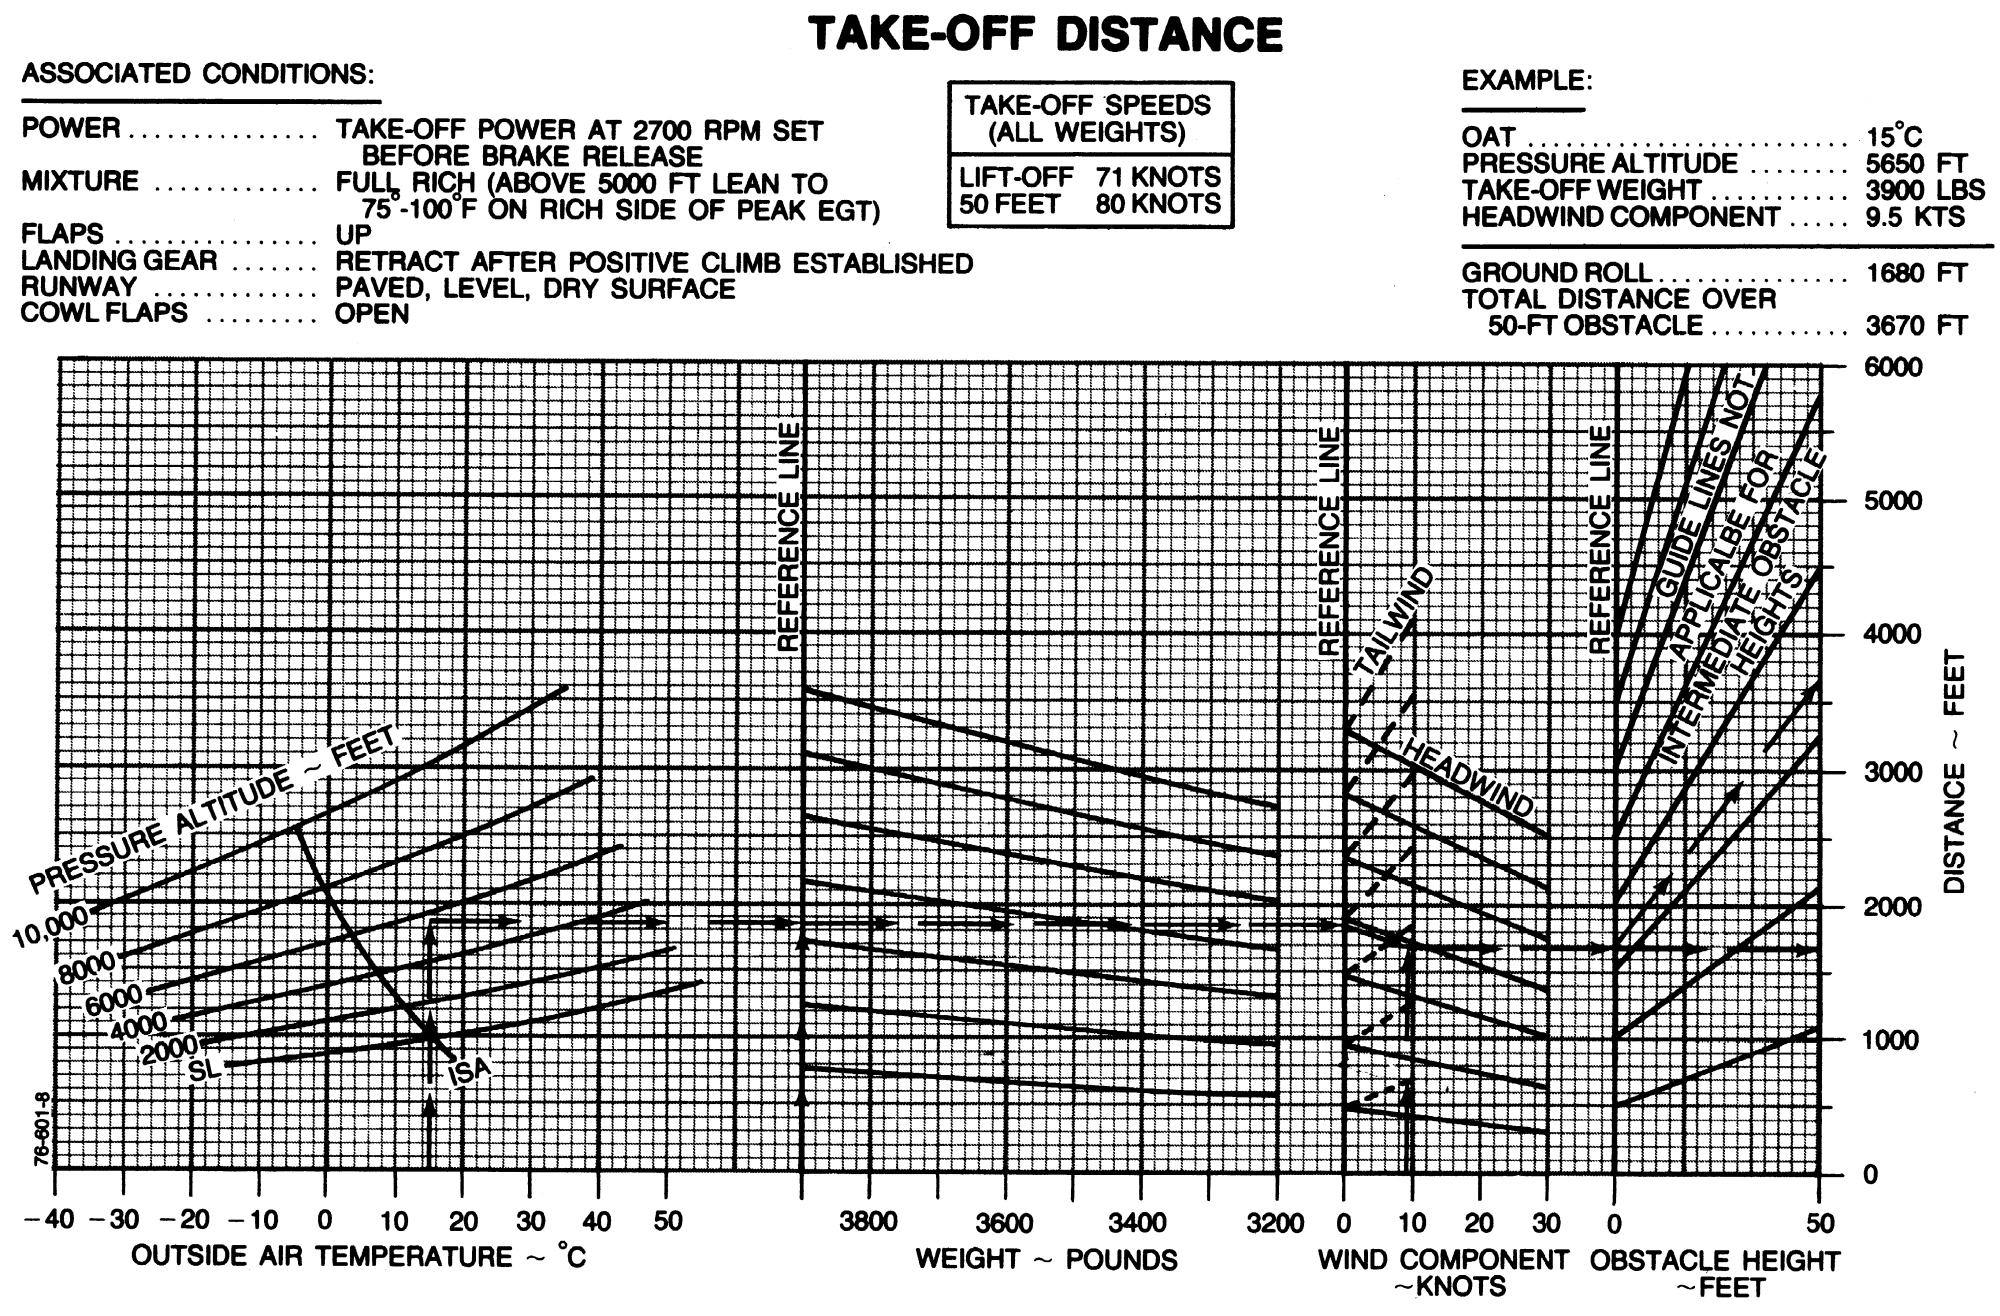
\includegraphics[width=0.95\linewidth]{duchess-takeoff-distance}
\end{center}
\end{figure}

\section{Accelerate-Stop Distance}

\begin{figure}[H]
\begin{center}
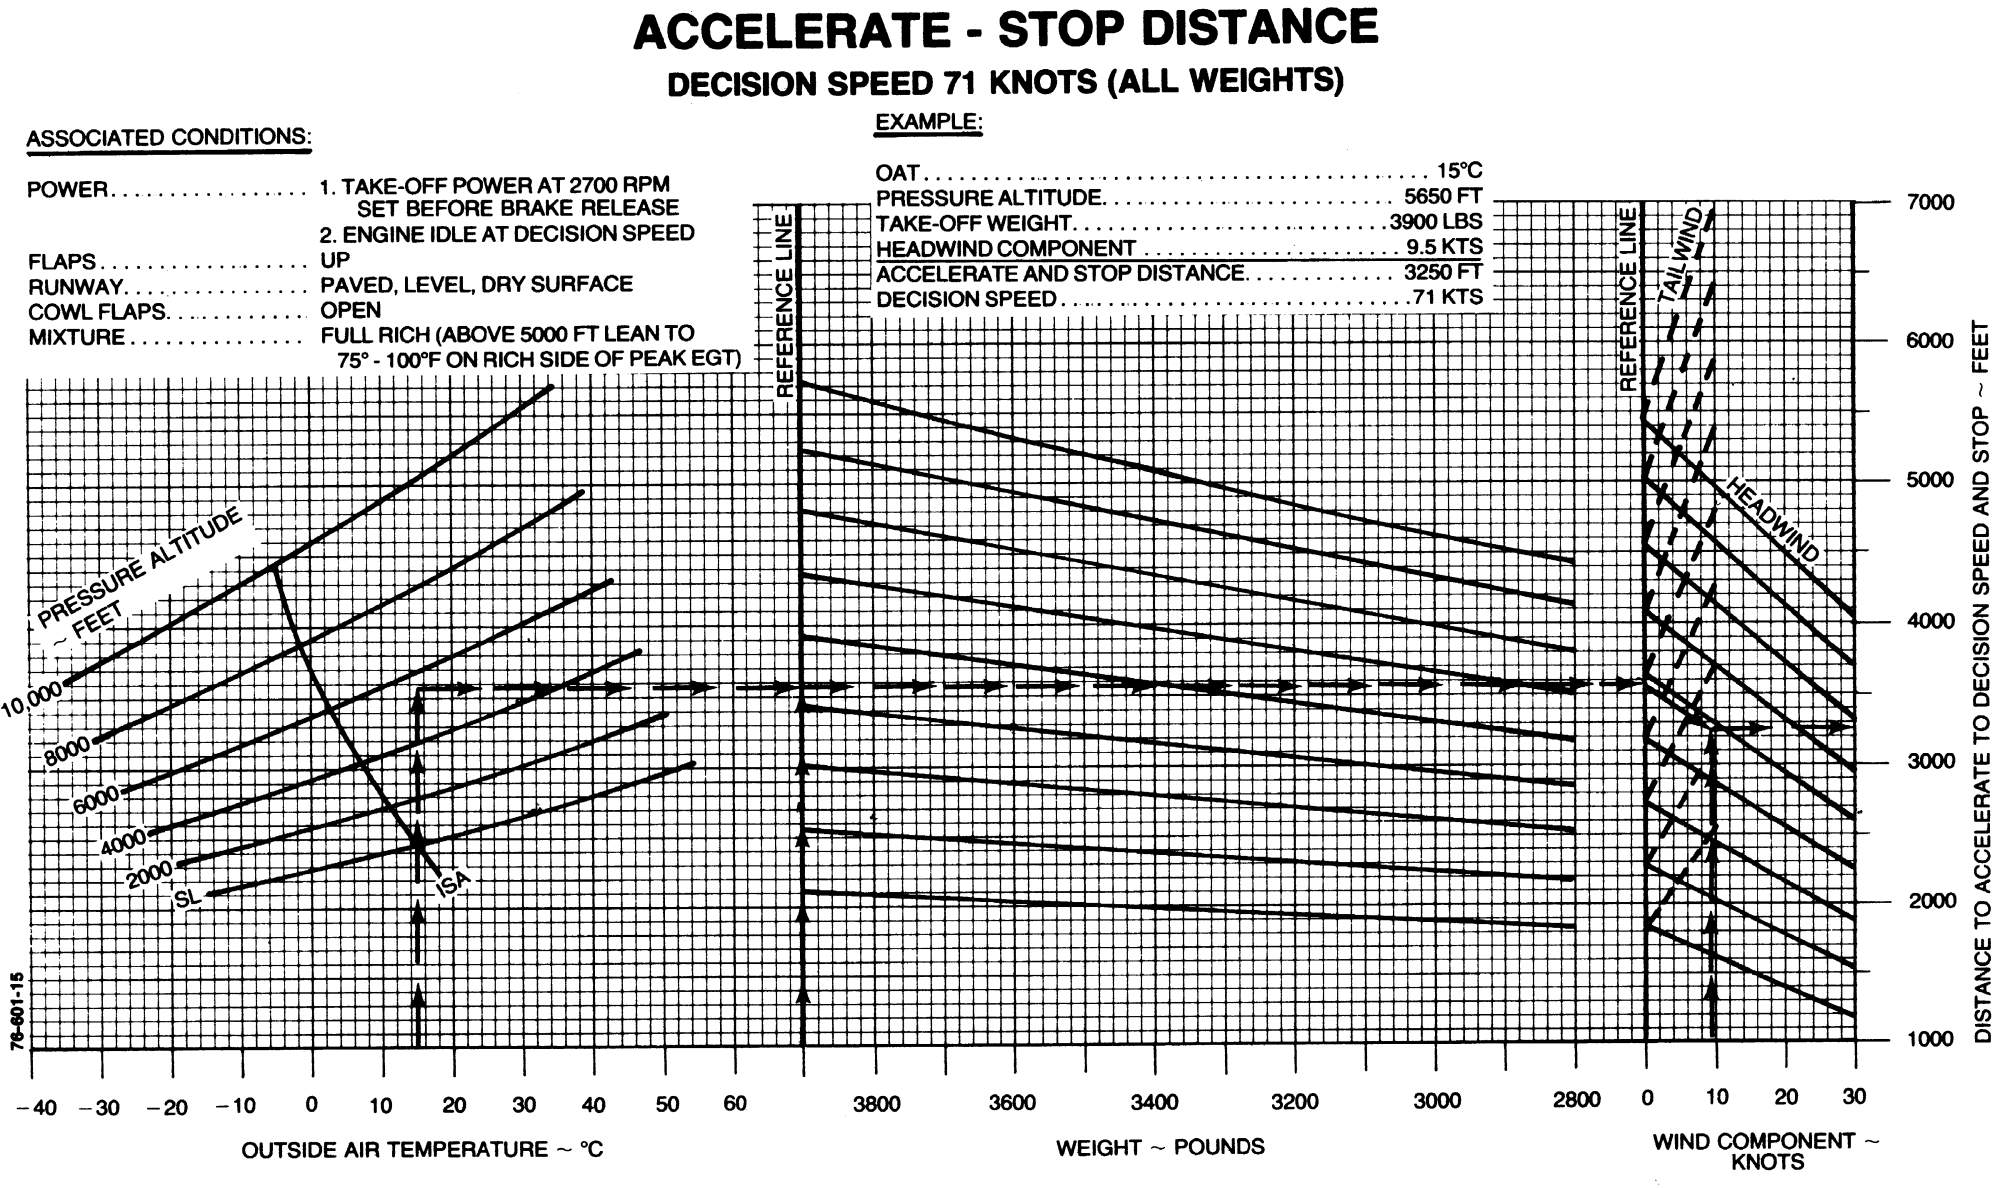
\includegraphics[width=0.95\linewidth]{duchess-asda}
\end{center}
\end{figure}

\section{Accelerate-Go Distance}

\begin{figure}[H]
\begin{center}
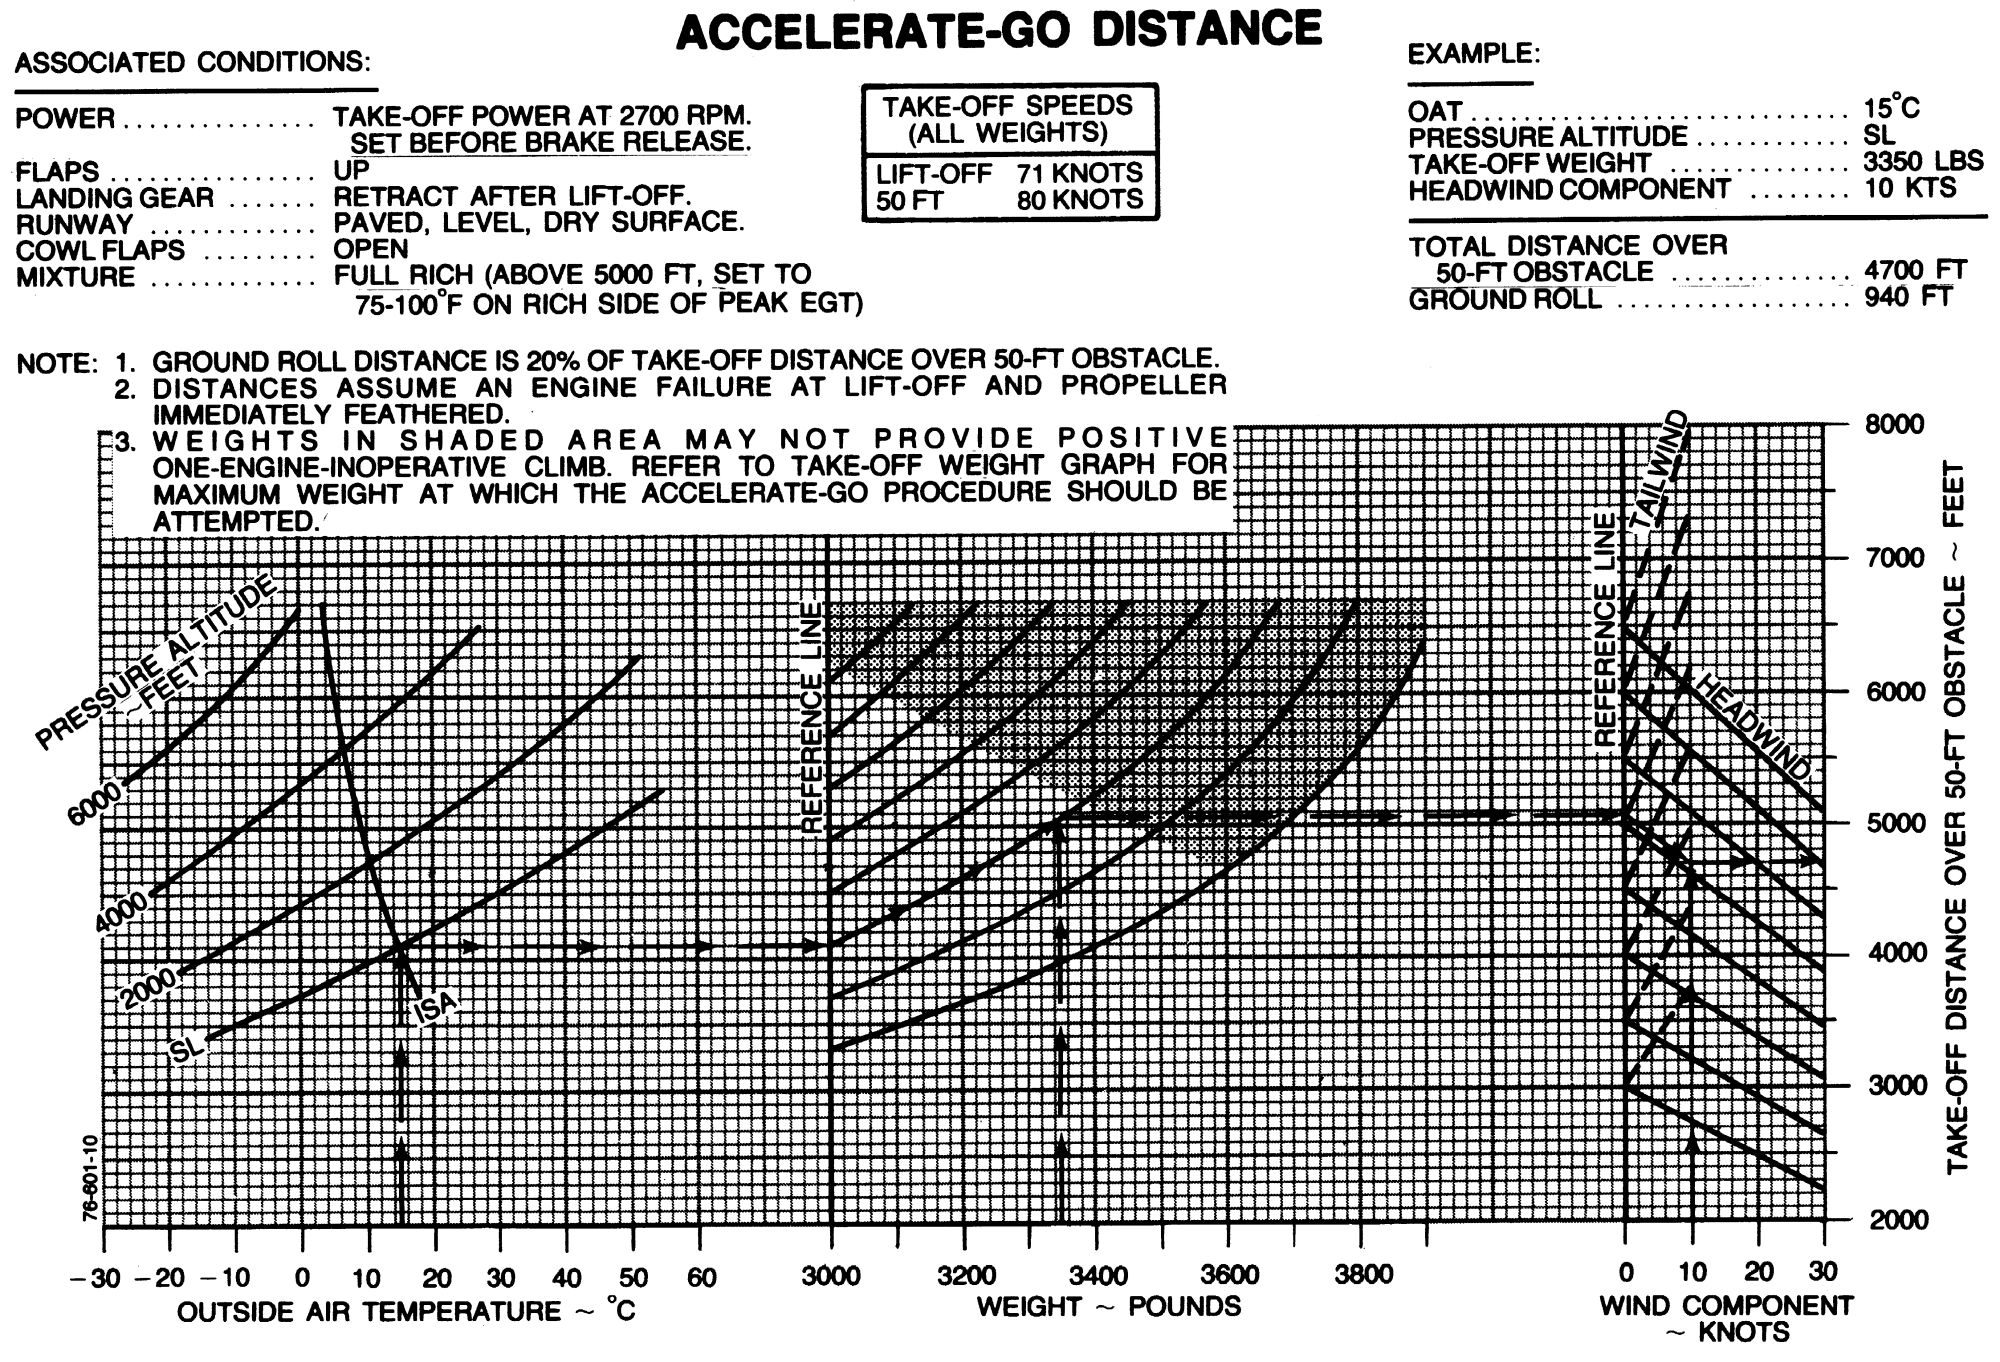
\includegraphics[width=0.95\linewidth]{duchess-accel-go}
\end{center}
\end{figure}

\newpage

\section{Two-Engine Climb Rate}

\begin{figure}[H]
\begin{center}
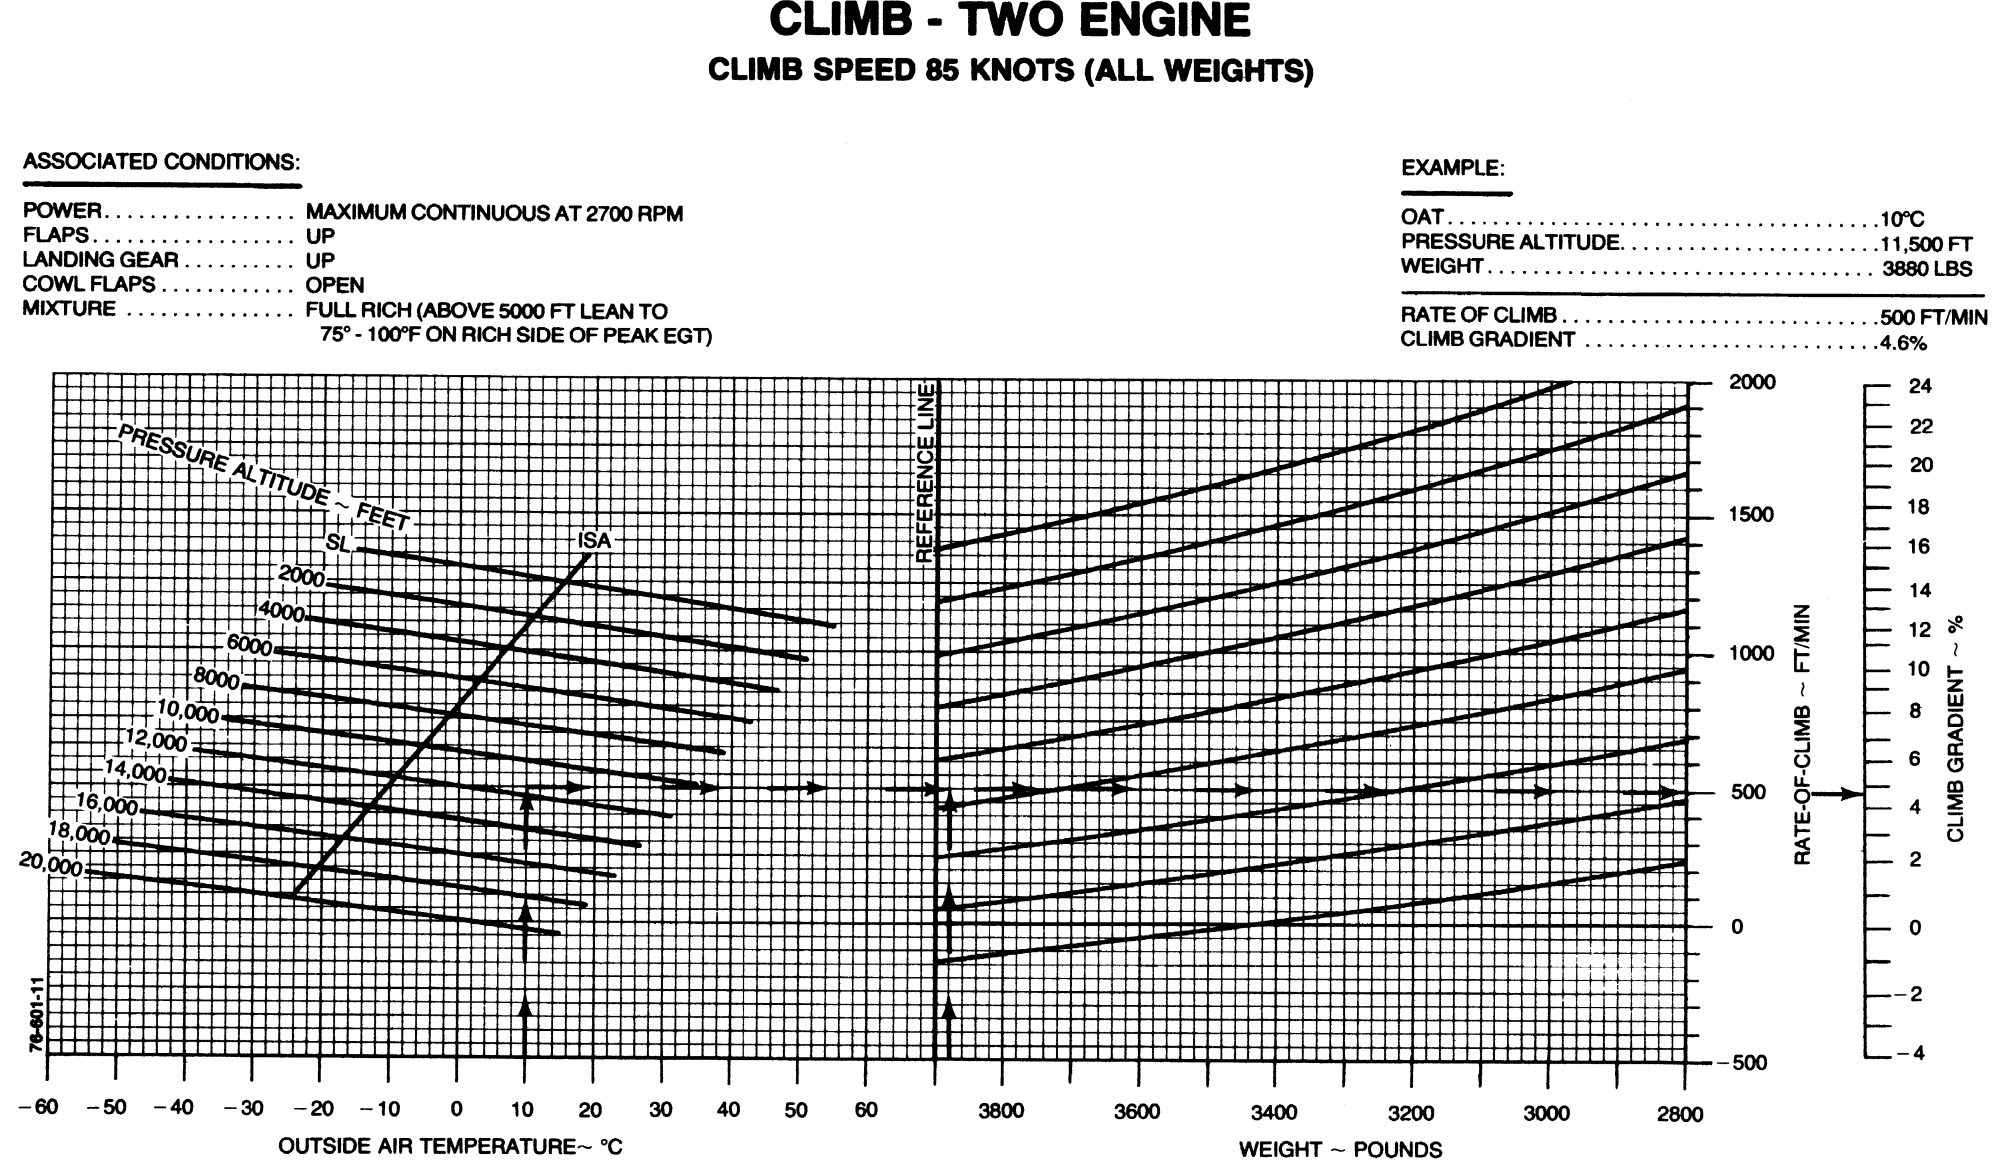
\includegraphics[width=0.9\linewidth]{duchess-2ec}
\end{center}
\end{figure}


\section{Single-Engine Climb Rate}

\begin{figure}[H]
\begin{center}
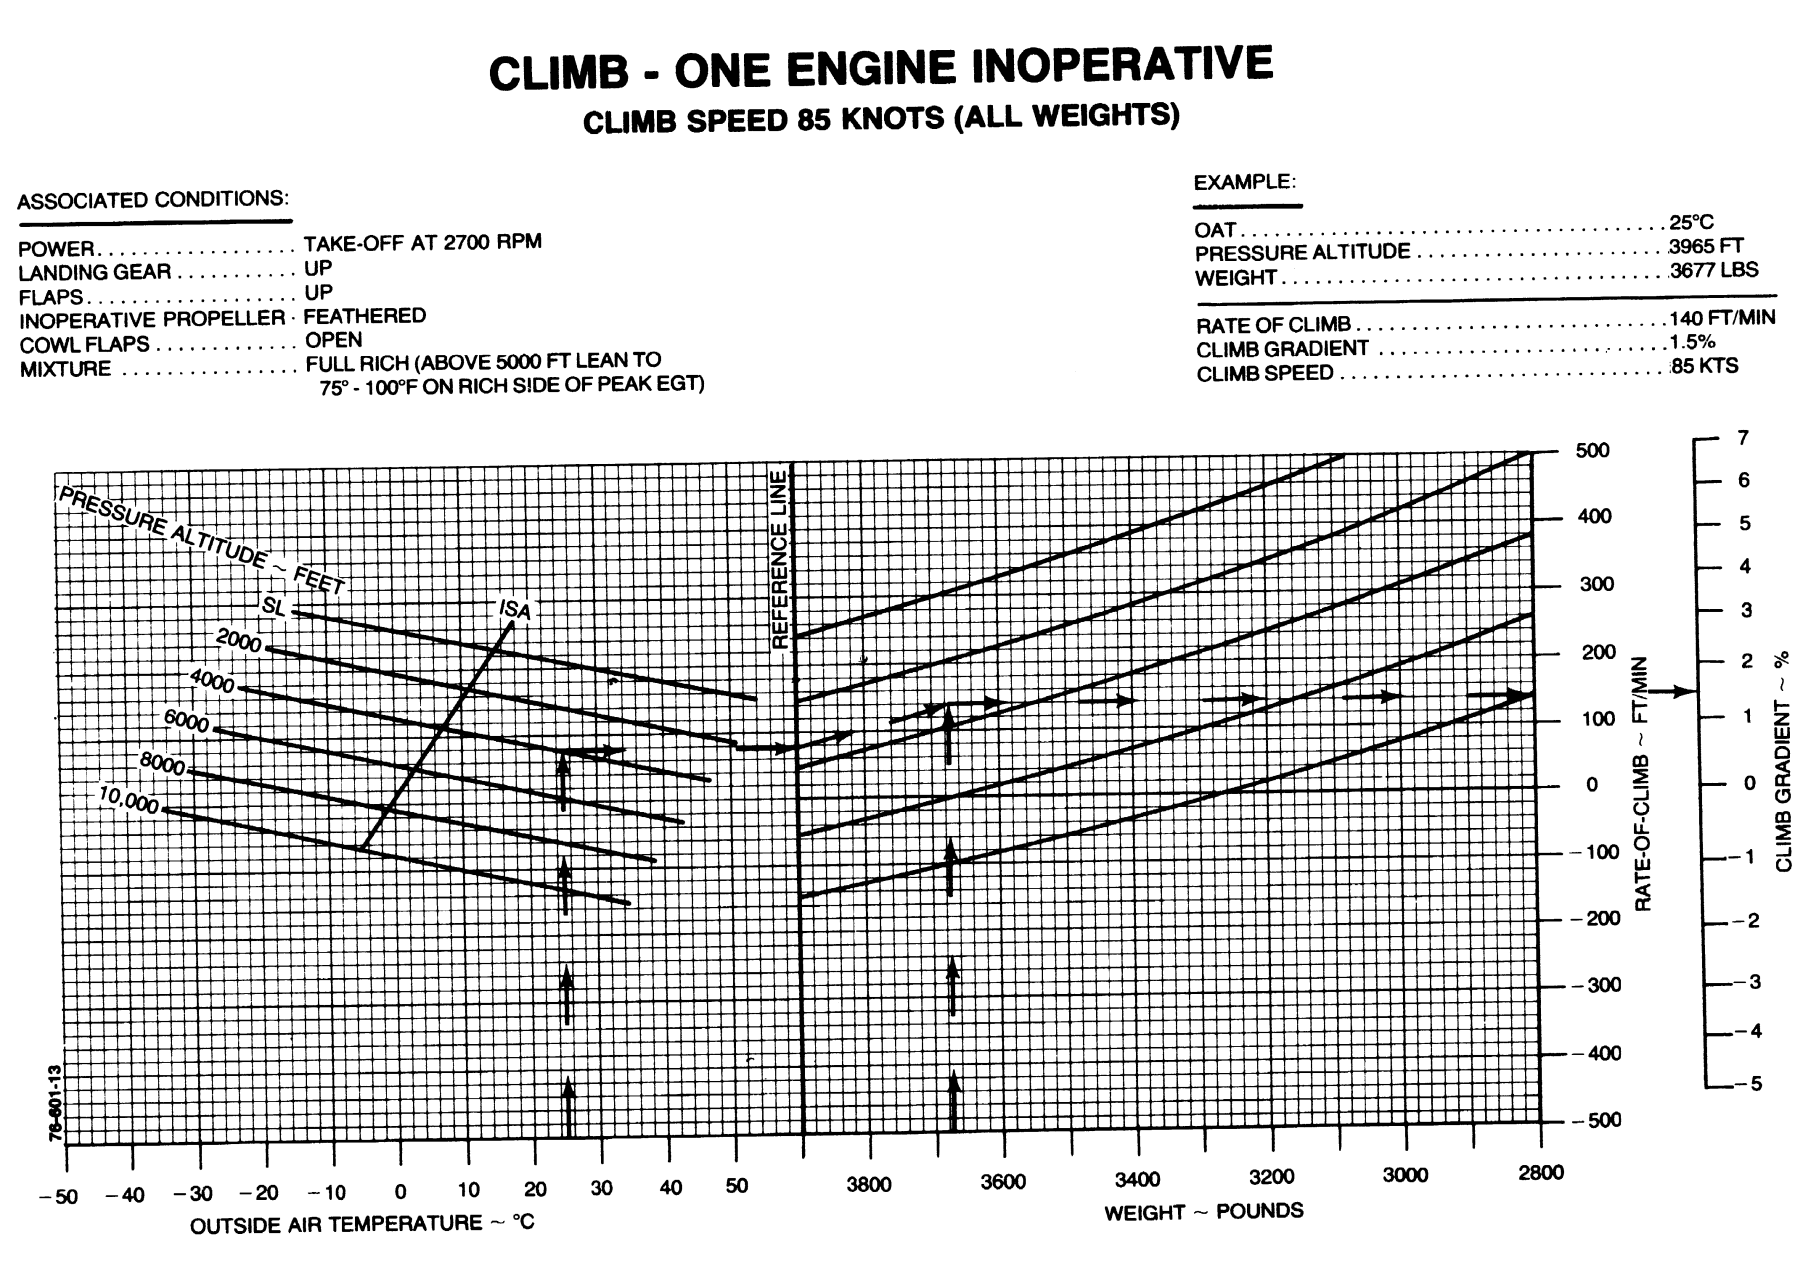
\includegraphics[width=0.9\linewidth]{duchess-1eo}
\end{center}
\end{figure}

\section{Time, Fuel, and Distance to Climb}

\begin{figure}[H]
\begin{center}
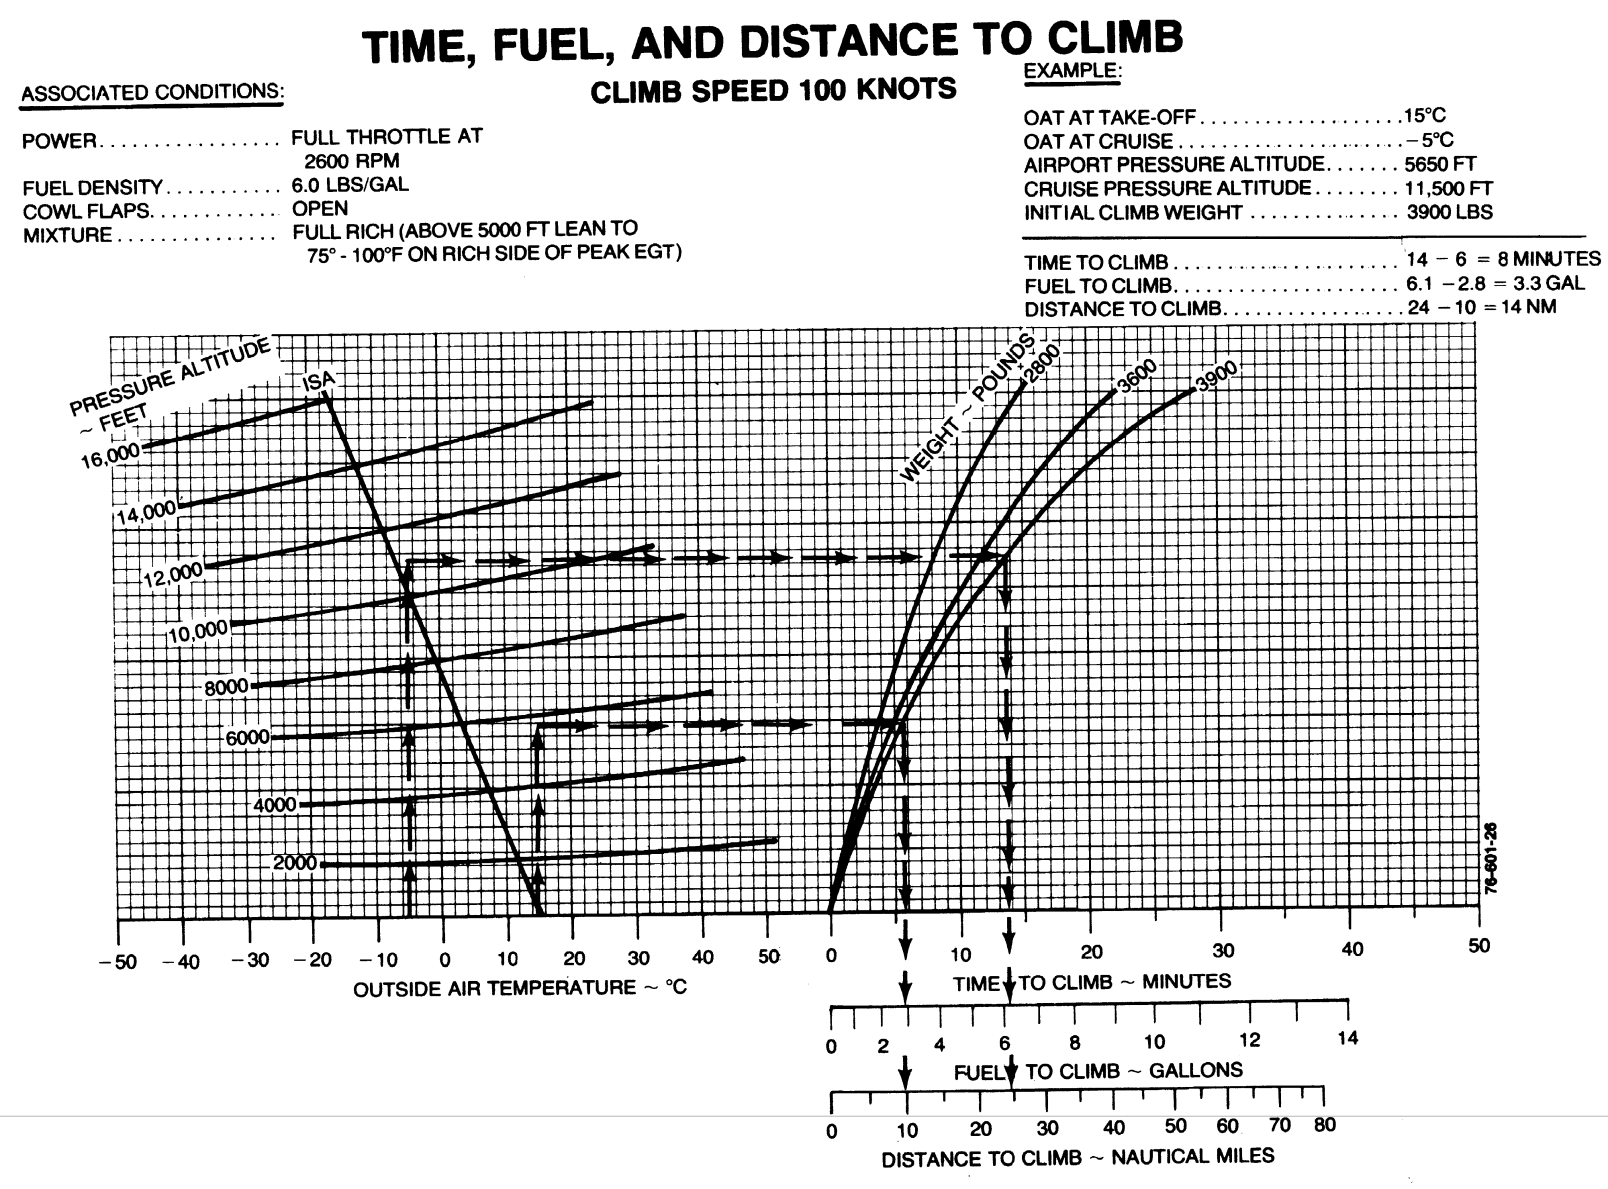
\includegraphics[width=1.0\linewidth]{duchess-tfd}
\end{center}
\end{figure}

\emph{Memory aid:}

\begin{table}[H]
\begin{tabular}{l|l|l|l}
      & \multicolumn{1}{c|}{\begin{tabular}[c]{@{}c@{}}min\\ T\end{tabular}} & \multicolumn{1}{c|}{\begin{tabular}[c]{@{}c@{}}gal\\ F\end{tabular}} & \multicolumn{1}{c}{\begin{tabular}[c]{@{}c@{}}nmi\\ D\end{tabular}} \\ \hline
4500  & 3.5                                                                  & 1.9                                                                  & 6                                                                   \\ \hline
GTU   & 0.2                                                                  & 0.1                                                                  & 1                                                                   \\ \hline
climb & 3                                                                    & 1.8                                                                  & 5                                                                  
\end{tabular}
\end{table}

\newpage

\section{Single-Engine Service Ceiling}

\begin{figure}[H]
\begin{center}
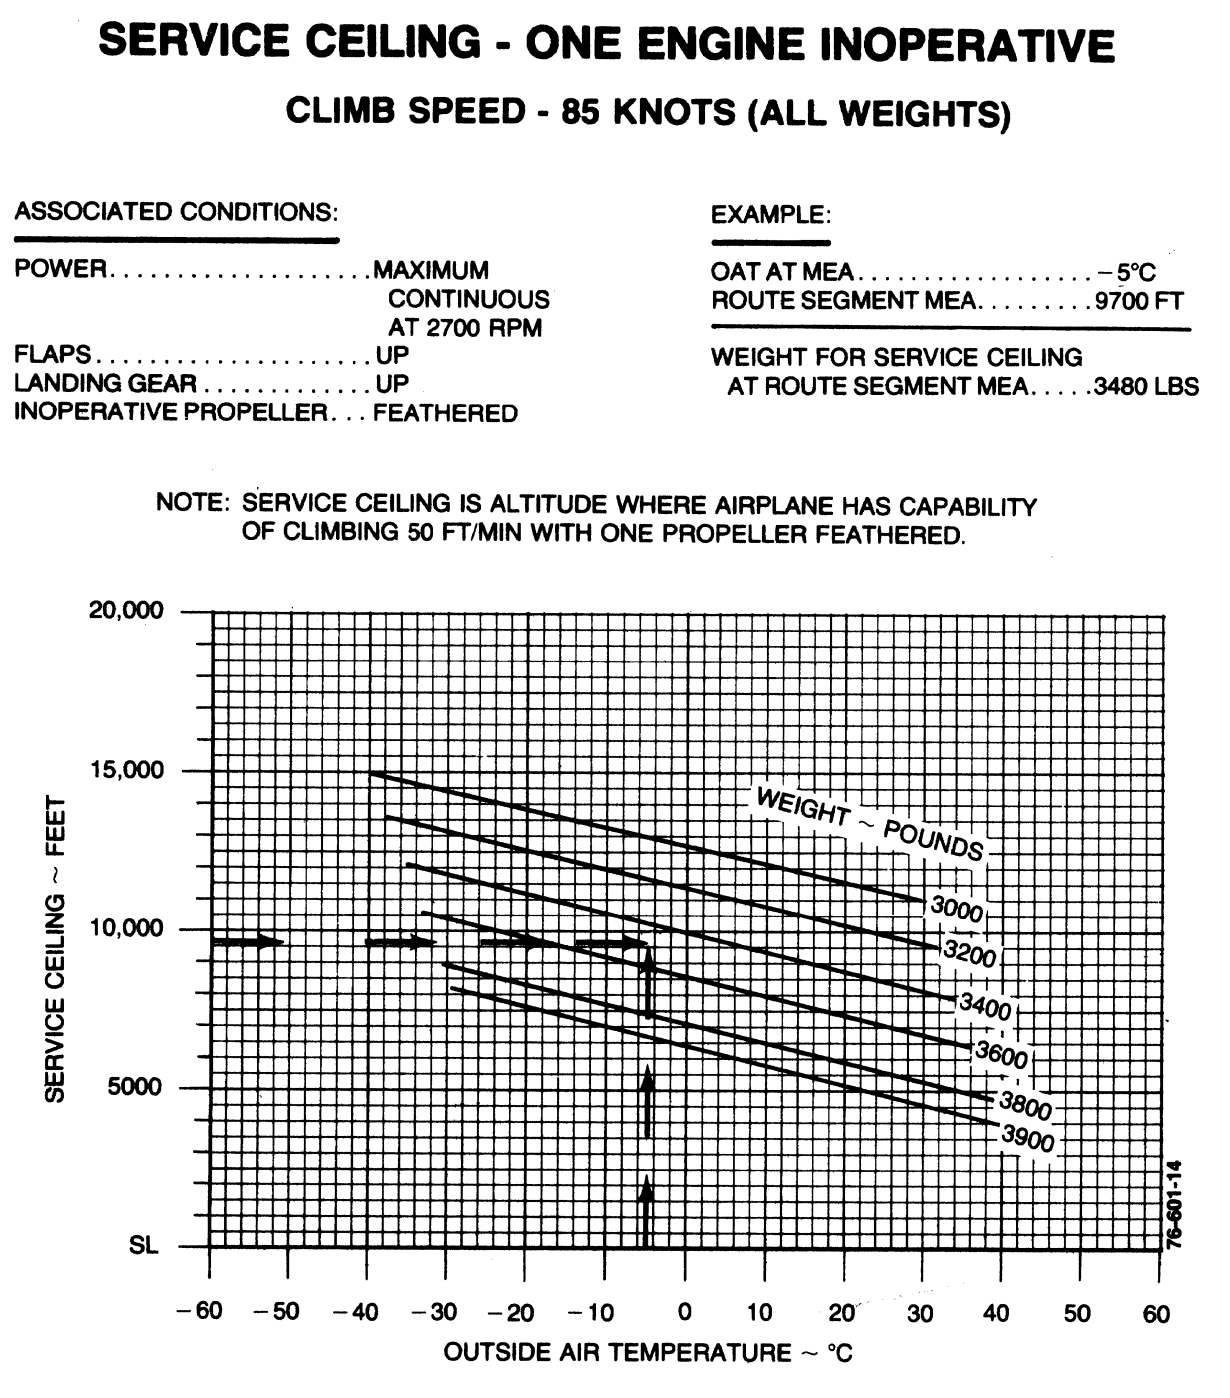
\includegraphics[width=1.0\linewidth]{duchess-secc}
\end{center}
\end{figure}

\newpage

\section{Cruise Performance, 24” Hg}

\begin{figure}[H]
\begin{center}
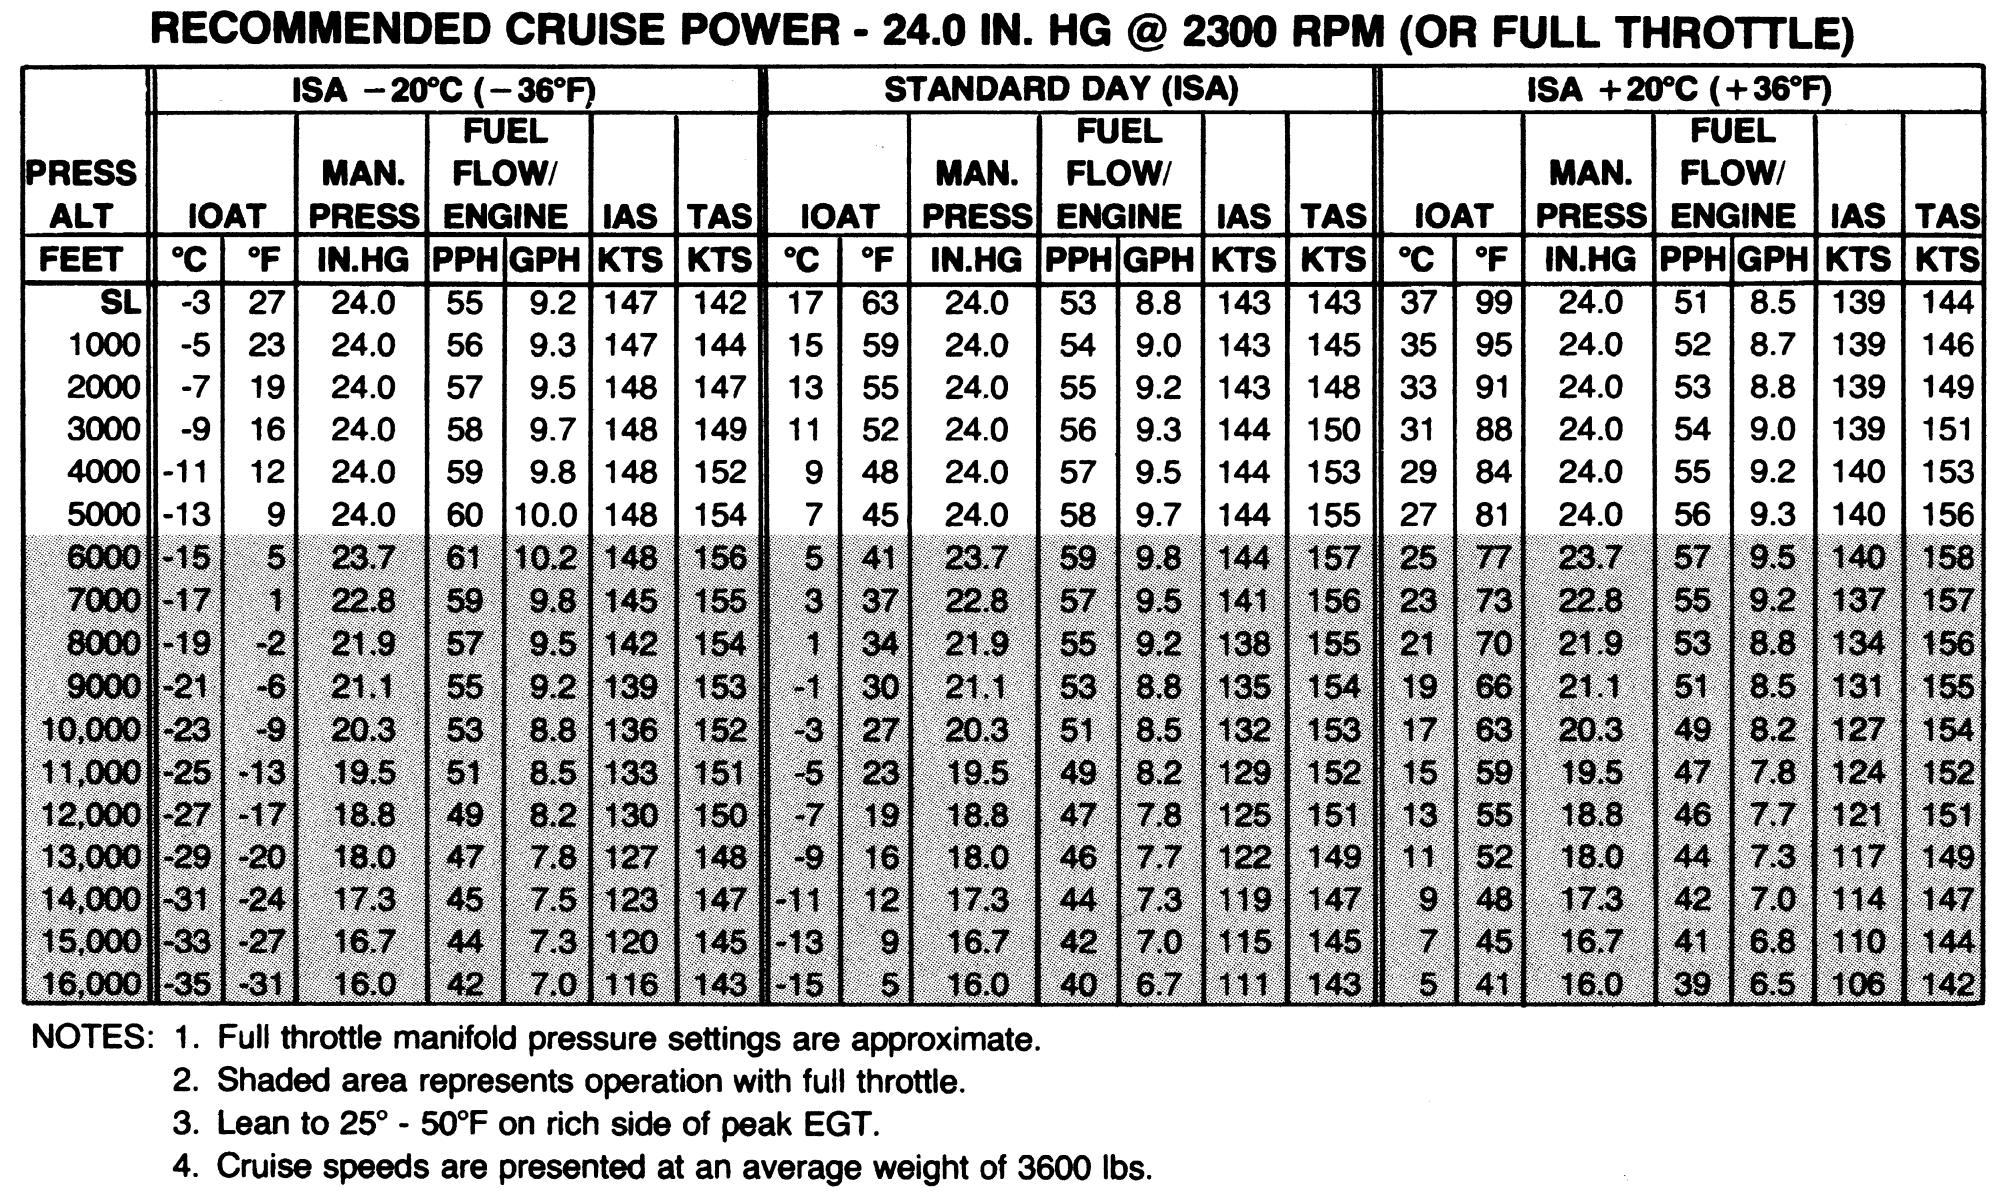
\includegraphics[width=0.9\linewidth]{duchess-24in}
\end{center}
\end{figure}

\section{Cruise Performance, 20” Hg}

\begin{figure}[H]
\begin{center}
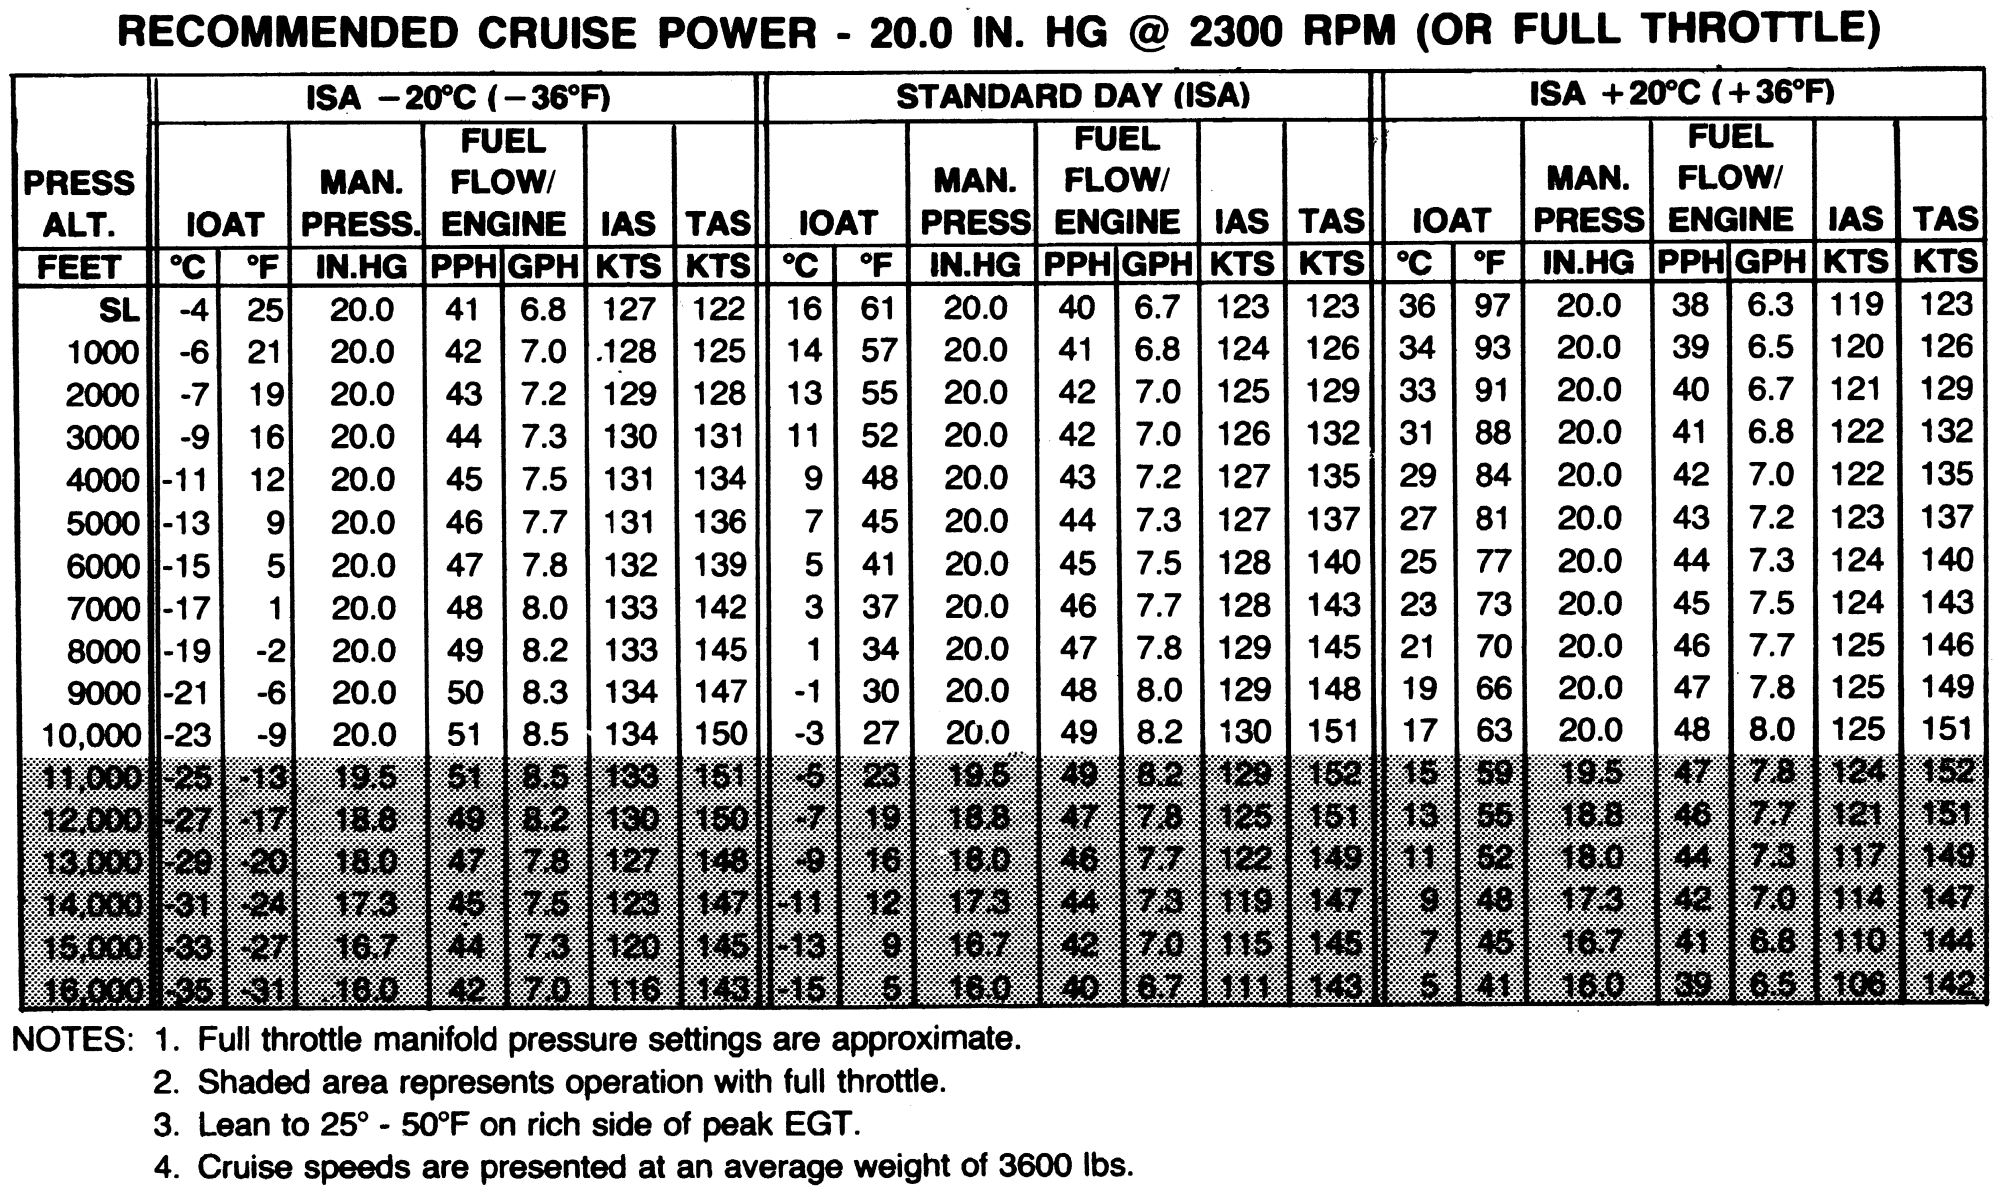
\includegraphics[width=0.9\linewidth]{duchess-20in}
\end{center}
\end{figure}

\newpage

\section{Landing Distance}

\begin{figure}[H]
\begin{center}
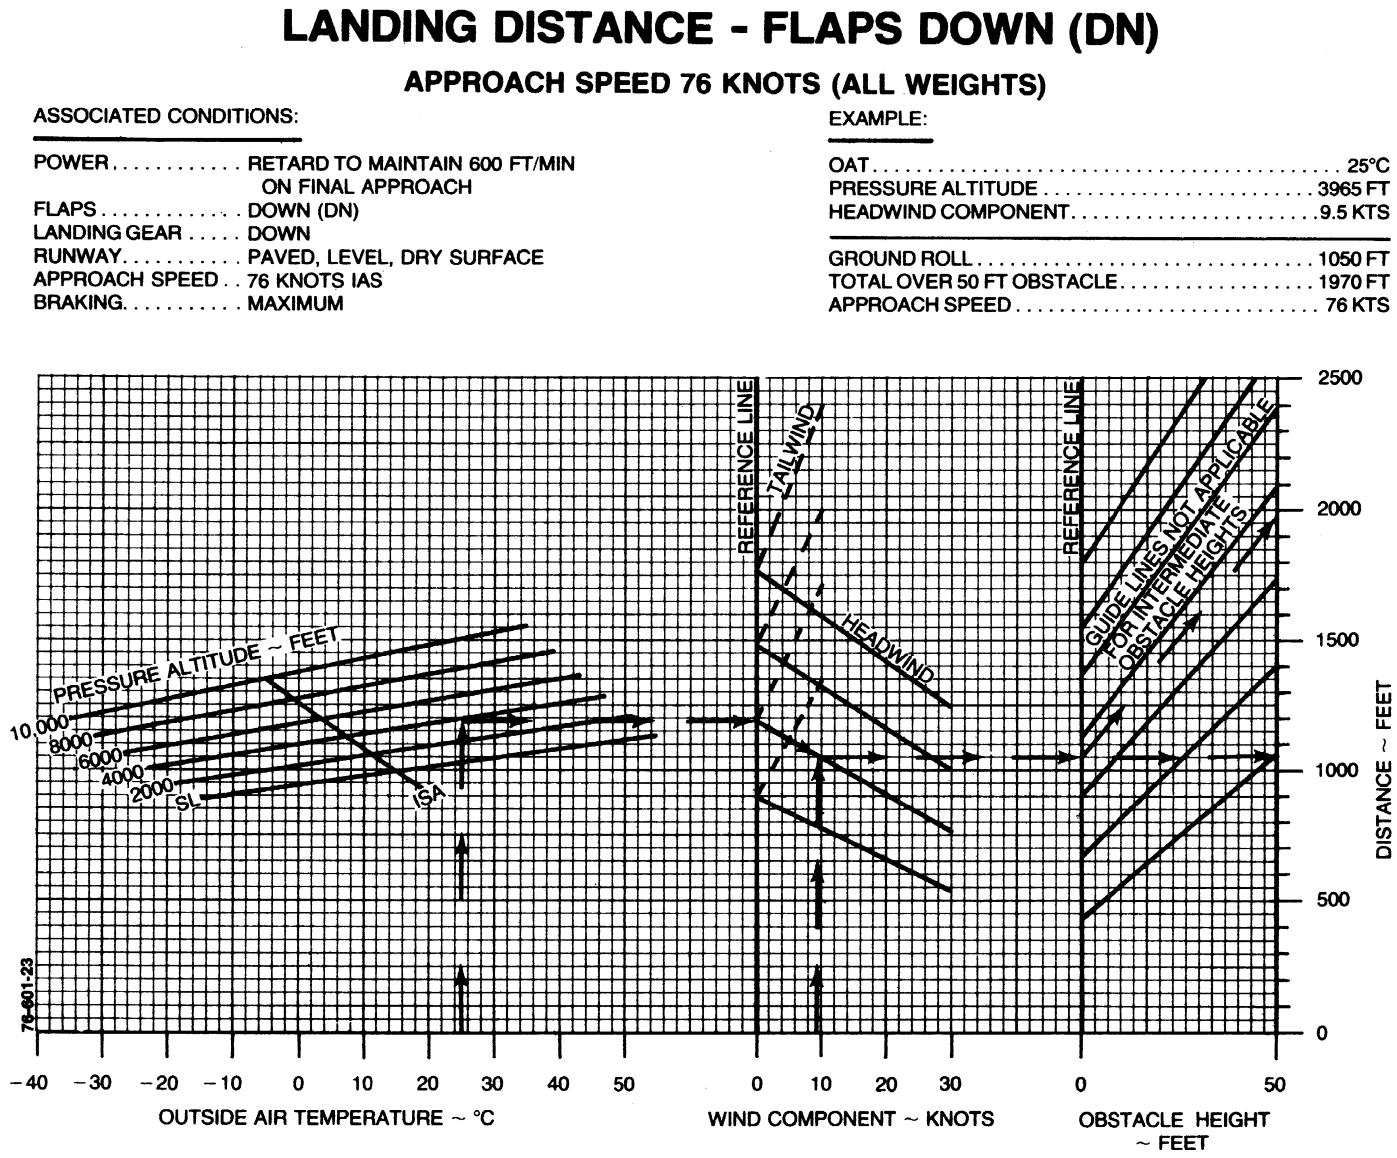
\includegraphics[width=1.0\linewidth]{duchess-ldg}
\end{center}
\end{figure}

\chapter{Weight and Balance}

Calculation of weight and balance in the Duchess is straightforward.
Note that the Duchess has a maximum zero
fuel weight, which restricts the useful load carried as passengers
and cargo. The maximum weight of the airplane
plus passengers and baggage must not exceed 3500 pounds – the rest
of the useful load must be carried as fuel.

See the figures available in the POH for information on loading arms and C.G. limits.

\begingroup
\renewcommand{\arraystretch}{1.1} % Default value: 1

\begin{table}[H]
\begin{tabular}%
  {>{\raggedright\arraybackslash}p{0.15\linewidth}%
   >{\centering\arraybackslash}p{0.2\linewidth}%
   >{\centering\arraybackslash}p{0.2\linewidth}%
   >{\centering\arraybackslash}p{0.2\linewidth}%
  }
                                                                                                        & \textbf{Weight}       & \textbf{x Arm}                                                                         & \textbf{= Moment}     \\ \cline{2-4} 
\multicolumn{1}{l|}{Basic Empty Condition}                                                              & \multicolumn{1}{c|}{} & \multicolumn{1}{c|}{}                                                                  & \multicolumn{1}{c|}{} \\ \cline{2-4} 
\multicolumn{1}{l|}{Pilot \& Front Passengers}                                                          & \multicolumn{1}{c|}{} & \multicolumn{1}{c|}{\begin{tabular}[c]{@{}c@{}}105 (forward)\\ 112 (aft)\end{tabular}} & \multicolumn{1}{c|}{} \\ \cline{2-4} 
\multicolumn{1}{l|}{Passengers – Row 2}                                                                 & \multicolumn{1}{c|}{} & \multicolumn{1}{c|}{144}                                                               & \multicolumn{1}{c|}{} \\ \cline{2-4} 
\multicolumn{1}{l|}{Baggage (200\# max)}                                                                & \multicolumn{1}{c|}{} & \multicolumn{1}{c|}{167}                                                               & \multicolumn{1}{c|}{} \\ \cline{2-4} 
\multicolumn{1}{l|}{\textbf{\begin{tabular}[c]{@{}l@{}}Zero Fuel Weight\\ (3500\# max)\end{tabular}}}   & \multicolumn{1}{c|}{} & \multicolumn{1}{c|}{}                                                                  & \multicolumn{1}{c|}{} \\ \cline{2-4} 
\multicolumn{1}{l|}{Fuel}                                                                               & \multicolumn{1}{c|}{} & \multicolumn{1}{c|}{117}                                                               & \multicolumn{1}{c|}{} \\ \cline{2-4} 
\multicolumn{1}{l|}{Ramp Condition}                                                                     & \multicolumn{1}{c|}{} & \multicolumn{1}{c|}{}                                                                  & \multicolumn{1}{c|}{} \\ \cline{2-4} 
\multicolumn{1}{l|}{Start/Taxi/Takeoff}                                                                 & \multicolumn{1}{c|}{} & \multicolumn{1}{c|}{}                                                                  & \multicolumn{1}{c|}{} \\ \cline{2-4} 
\multicolumn{1}{l|}{\textbf{\begin{tabular}[c]{@{}l@{}}Takeoff Condition\\ (3900\# max)\end{tabular}}}  & \multicolumn{1}{c|}{} & \multicolumn{1}{c|}{}                                                                  & \multicolumn{1}{c|}{} \\ \cline{2-4} 
\multicolumn{1}{l|}{Load Adjustments:}                                                                  & \multicolumn{1}{c|}{} & \multicolumn{1}{c|}{}                                                                  & \multicolumn{1}{c|}{} \\ \cline{2-4} 
\multicolumn{1}{l|}{Front seat}                                                                         & \multicolumn{1}{c|}{} & \multicolumn{1}{c|}{\begin{tabular}[c]{@{}c@{}}105 (forward)\\ 112 (aft)\end{tabular}} & \multicolumn{1}{c|}{} \\ \cline{2-4} 
\multicolumn{1}{l|}{Passenger}                                                                          & \multicolumn{1}{c|}{} & \multicolumn{1}{c|}{144}                                                               & \multicolumn{1}{c|}{} \\ \cline{2-4} 
\multicolumn{1}{l|}{Baggage}                                                                            & \multicolumn{1}{c|}{} & \multicolumn{1}{c|}{167}                                                               & \multicolumn{1}{c|}{} \\ \cline{2-4} 
\multicolumn{1}{l|}{Fuel}                                                                               & \multicolumn{1}{c|}{} & \multicolumn{1}{c|}{117}                                                               & \multicolumn{1}{c|}{} \\ \cline{2-4} 
\multicolumn{1}{l|}{\textbf{\begin{tabular}[c]{@{}l@{}}New Takeoff Weight\\ (3900\# max)\end{tabular}}} & \multicolumn{1}{c|}{} & \multicolumn{1}{c|}{}                                                                  & \multicolumn{1}{c|}{} \\ \cline{2-4} 
\multicolumn{1}{l|}{Fuel Burn}                                                                          & \multicolumn{1}{c|}{} & \multicolumn{1}{c|}{117}                                                               & \multicolumn{1}{c|}{} \\ \cline{2-4} 
\multicolumn{1}{l|}{\textbf{Landing Condition}}                                                         & \multicolumn{1}{c|}{} & \multicolumn{1}{c|}{}                                                                  & \multicolumn{1}{c|}{} \\ \cline{2-4} 
\end{tabular}
\end{table}
\endgroup


\chapter{Systems - Beechcraft Duchess BE-76}

\emph{Memory aid: N6001Y ME-119; N3733G ME-364}

\section{Engines}

The Duchess has two Lycoming 4 cylinder-engines – an O360 on the left, and an LO-360 (the ``L'' is for ``left'' turning) on the right. Both engines produce 180 horsepower at 2700 RPM and are air-cooled, direct drive,
horizontally opposed, reciprocating, normally aspirated engines. Oil capacity is 8 quarts maximum.

\section{Propellers}

\subsection{Propeller System Basics}

The Duchess has two 76-inch diameter, constant speed, full-feathering Hartzell propellers. The propellers are
counter-rotating: the left propeller turns clockwise and right propeller turns counterclockwise. Unlike most light
twins which have conventional propellers where both turn clockwise, there is no critical engine with counter-
rotating propellers. See the definition of critical engine in Section 1.

The propeller controls on the control console allow the pilot to select the governor's RPM range. Propeller governors
regulate oil pressure to control RPM by varying the blade angle (pitch) of the propeller to make it more efficient.
Oil pressure and aerodynamic twisting send the propeller out of feather to high RPM settings (low pitch=small blade
angle, taking small ``bites'' of air). Nitrogen pressure and a large spring, aided by counterweights, send the propeller
to low RPM (high pitch=high blade angle).

The oil pressure and nitrogen/spring pressure constantly oppose each other. When the propeller control is moved to
the feather position, the opposing oil pressure is released and the spring, air pressure and counterweights cause the
propeller to ``feather'' - a pitch of approximately 80\degree; this is a minimum drag condition. The propellers can be
unfeathered with the aid of unfeathering accumulators. When the propeller control is moved forward, stored oil
pressure is released which forces the propeller into a lower pitch. If this is done above 100 knots, the propeller
should windmill, allowing the engine to be re-started without the aid of the starter.

A feathering lock, operated by centrifugal force, prevents feathering during engine shut down by making it
impossible to feather any time the engine speed falls below 950 RPM. For this reason, when the pilot wishes to
feather a propeller, he must be sure to move the propeller control into the FEATHER position before the engine
speed drops below 950 RPM. This will not happen while airborne since the propeller will windmill faster than 950
RPM with normal propeller control settings. \emph{(see schematic)}

\subsection{Propeller Governor Operation}

The propeller governor is mounted on the accessory case on the rear of the engine. It contains a speeder spring,
which is directly controlled by the propeller lever in the cockpit, and flyweights which spin at engine RPM (see
propeller system diagram). When the pilot sets an RPM value with the propeller control, the engine attempts to
maintain that RPM setting by pitching the blades as required by the existing airspeed and power setting.

The propeller governor operates by regulating the flow of high-pressure oil into and out of the propeller hub.
Increasing oil pressure into the hub pitches the propeller blades flatter (higher RPM) and allowing oil to flow out of
the propeller hub allows the propeller to achieve a higher pitch (lower RPM or feather). The flow of oil is controlled
by a pilot valve in the governor which blocks the flow of oil to and from the propeller hub under normal conditions.

When the propeller RPM starts to increase (because of a momentary dive, for example) the flyweights are slung
away from the rotating shaft because of centrifugal force. This raises the shaft, which allows oil to flow from the
propeller hub to the oil sump, moving the blades to higher pitch and reestablishing the set RPM value. When the
propeller RPM starts to decrease, the counterweights have less centrifugal force slinging them away from the shaft,
and the speeder spring forces them inward. This moves the pilot valve in the opposite direction, which allows the
flow of high-pressure oil into the propeller hub, moving the blades to a flatter position and increasing RPM to the set
value.

At lower power settings and airspeeds, the propellers may be fully flat and RPM will decrease below the set value.
At this point, moving the propeller control fully forward will have no effect on engine RPM, since the blades are
already at their flattest pitch.

\emph{Memory aid: This is why the throttles change RPM when at idle.}

\section{Landing Gear}

The retractable tricycle landing gear uses shock absorbers on the main gear (approximately 2" extension) and an
oleo strut on the nose gear (approximately 4 1/4" extension) for shock absorption. The nose gear is steerable
through a spring-loaded linkage connected to the rudder pedals. A hydraulic dampener on the nose strut eliminates
shimmy. Toe brakes aid in steering the aircraft. The minimum wingtip turn radius is approximately 27' with the use
of differential power.

Retraction and extension of the gear is accomplished through the use of an electrically driven reversible hydraulic
pump and hydraulic system terminating in a hydraulic actuator assembly mounted in each wheel well. Retraction or
extension requires 6-8 seconds. The gear is held in the retracted position by 1250 to 1550 PSI of hydraulic pressure;
there are no locks to hold the gear in the retracted position. The landing gear may be hydraulically extended or
retracted, and may be lowered manually (below 100 knots) by turning a dump valve which releases pressure from
the retract side of the system allowing the gear to free fall to the down and locked position. If you lose hydraulic
pressure for some other reason, the gear will lower (free fall) to the down position and you will not be able to raise
it. If you lose electrical power the gear can be lowered manually but not raised. For any gear malfunction
ALWAYS refer to the checklist.

\emph{Memory aid: Gear is electrically driven, hydraulically actuated. Pressure holds it up. Lack of pressure causes gear to free fall. That lets us drop gear in an emergency.}

Three green lights, one for each landing gear, are illuminated whenever the landing gear are down and locked. The
red light illuminates any time the gear is in transit, indicating that the hydraulic pump is active. All of the lights will
be extinguished when the gear is up. Pressing the face of each indicator light will verify that the lights are
functional. The intensity of the lamps can be controlled by turning the lens holder on each lamp (counterclockwise
is brighter, full clockwise will appear that the bulb is out). In addition, the 4 gear indicator lights are
interchangeable with each other to verify that you do not have a burned out bulb.

In the retract mode the electric pump/motor forces hydraulic fluid to the retract side of the system. A pressure
switch shuts off the motor (and extinguishes the red in-transit light) when the system pressure reaches approximately
1550 PSI. If pressure drops to approximately 1250 PSI the motor will again be activated, and the red in-transit light
will illuminate. An uplock check valve in the pump retains this pressure to hold the gear up. In addition, landing
gear retraction operation is protected by a time-delay relay, which will disengage electrical power to the pump/motor
after 30 seconds of continuous operation. If the landing gear in-transit light remains illuminated, it indicates
improper response of the landing gear. The relay can be reset by moving the gear switch to the down position.

\emph{Memory aid: Watch for gear in transit light illuminating in flight, this could indicate a failing pump or a leak in the system.}

In the extend mode the electric motor forces hydraulic fluid to the extend side of the system. Main gear downlock is
accomplished by over-center travel of a spring-held side brace. Nose gear downlock is accomplished by over-center
travel of the drag link and a mechanically actuated downlock. After the gear are down and locked, system pressure
will bleed back to zero. Down limit switches, located on each gear, will allow the pump/motor to run until all three
gear are down and locked.

To prevent inadvertent retraction of the landing gear on the ground, a safety pressure switch is installed in the pitot
system to deactivate the hydraulic pump circuit when impact air pressure is below approximately 59 to 63 knots.

\emph{Memory aid: Do not retract the gear on the ground! What if the safety pressure switch is inoperative?}

If either or both throttles are retarded below an engine setting sufficient to sustain flight and the landing gear are not
fully extended, the landing gear warning horn will sound intermittently. An optional gear warning silence button
\emph{(not installed in either of the PCA Duchess aircraft as of this writing)}
allows the pilot to silence the alarm if one throttle is retarded. Additionally, when the flaps are extended beyond
about 16\degree, the warning horn will sound, regardless of throttle position, if the landing gear is not down and locked.
\emph{(see schematic)}

System Operation Notes:
\begin{enumerate}
\item The pilot moves the propeller control, which applies or relieves pressure from the speeder spring.
\item Flyweights and speeder spring move up and down, pushing or opening the pilot valve.
\item Oil from the engine driven governor oil boost pump is pushed toward the pilot value.
\item Oil moves past the pilot valve toward the propeller hub.
\item Oil fills the propeller hub in the direction of the low pitch stop.
\item The low pitch stop sets the high RPM limit.
\end{enumerate}

\section{Brakes and Tires}

Single-disk, double-piston Cleveland hydraulic brakes are fitted to the main gear. Each rudder pedal is fitted with a
master cylinder, which pressurizes the two pistons on either of the brake assemblies, forcing the linings to press
against the disk. To set the parking brake, pull the control out and pump both toe pedals until solid resistance is felt.
Push the control in to release the brakes. The hydraulic brake fluid reservoir is accessible through the nose
compartment. Fluid level is checked with the attached dipstick. The hydraulic system for the brakes is independent
of the gear. The main gear have 6.00-6 tires, and the nose gear has 5.00-5 tires. Normal inflation is 38 PSI for all
tires.

\section{Flaps and Trim}

Electrically actuated wing flaps are controlled by a three-position switch: UP, OFF, and DOWN. A dial type
indicator has position markings for UP, 10, 20, and DN (max is 35\degree{}). Limit switches interrupt power to the motor
when the flaps reach the extremes of travel. Intermediate flap positions can be obtained by placing the switch in the
off position during extension or retraction. Additionally, there is a micro switch activated at the 16\degree{} position which
is connected to the gear and stall warning circuits.

The elevator and rudder have cable-operated flight-adjustable trim tabs. The aileron control system has a trimmer
which functions by applying tension on the aileron control cables. Each control incorporates a mechanical position
indicator. The elevator trim may be operated manually or electrically.

\emph{Memory aid: $V_{FE}$ 120 KIAS @ 10 \degree{} - 20 \degree{}, 110 KIAS @ 35 \degree.}

\section{Pressure (Pneumatic) System}

Pressure for the attitude indicator and directional gyro is supplied by two engine-driven dry pressure pumps,
interconnected to form a single system. This is different from many light planes, which use vacuum to draw air
through the gyro instruments. If either pump fails, check valves automatically close and the remaining pump
continues to pressurize the system. Two red buttons on the pressure gauge indicate if that pump has failed. The HSI
is operated by the electrical system and therefore is not affected by a failure in the vacuum system.
\emph{(see schematic)}

\section{Pitot-Static System}

The Pitot tube is located outboard on the left wing. Pitot heat is available. The pitot system incorporates a pressure
switch, which prevents inadvertent gear retraction under approximately 60 knots. Static air is taken from flush static
ports located on each side of the fuselage. The alternate static air source is selectable on the lower left sidewall.
This lever also functions as the static system drain.

\section{Stall Warning System}

A stall warning sensing vane is installed on the leading edge of each wing. With flap settings of 0-15\degree{} the vane on
the left wing activates the warning horn. With flap settings of 16\degree{} or more the vane on the right wing activates the
system.

\section{Fuel System}

The airplane is designed for operation on grade 100 (green) or 100LL (blue) aviation gasoline. Two wing tanks hold
103 total gallons (100 usable). The filler neck of each tank contains a visual measuring tab to facilitate partial
filling. The sump drain on each tank can be locked open to offload fuel. There are eight fuel drain points. Each
engine has an engine driven fuel pump and an electrically driven boost pump, which serves as a backup and is used
for engine starts, takeoff, and landing. There are 3 positions on each fuel selector (on, off, and crossfeed). In
crossfeed, the engine will draw fuel from the opposite side in order to maintain a fuel balance during single engine
operations. Crossfeed should be used in level flight only. Each magneto/start switch incorporates a PUSH TO
PRIME function to aid in engine starting. A minimum of 9 gallons is required in each wing prior to takeoff.
\emph{(see schematic)}

\section{Heater and Defrost System}

A 45,000 BTU-per-hour combustion air heater, located on the right side in the nose compartment, provides heated
air for cabin warming and windshield defrosting. The heater system consists of a combustion air heater, a three-
position control switch, three push-pull control knobs, a heater circuit breaker, a manual reset limit (overheat) switch
(inaccessible in flight), a combustion air blower, a ventilation air blower, and a duct thermostat. The system uses
two thirds of a gallon per hour of fuel from the right wing. To operate, the cabin air outlet must be at least halfway
open.

\emph{Memory aid: The heater is deactivated in PCA aircraft. The external heater intake vents are covered for cold weather operations.}

\section{Electrical System}

\emph{Memory aid: N6001Y ME-119; N3733G ME-364}

One 24-volt, 15.5 ampere-hour, lead-acid battery is installed in the vented battery compartment just aft of the rear
bulkhead. Two self-exciting 55 ampere (for ME-183 and after, 28-volt: \textbf{N3733G}), or 60 ampere (for ME-1 thru ME-182, 14-
volt: \textbf{N6001Y}) belt driven alternators are installed, one on each engine. The systems are completely separate except for a bus
tie fuse, the mutual tie to the battery bus through two bus isolation circuit breakers, and the paralleling circuit
between the two voltage regulators (which makes sure the electrical load is equally shared between the two
alternators and keeps the voltage at 28 or 14 volts, depending upon the system installed). There are two load meters,
two pairs of alternator-out warning lights for over- or under-voltage conditions, and two over voltage relays which
will take the alternator off-line if the system exceeds operating voltage. The self-excitation feature will not come on
until approximately 1400 RPM, with a load capability of approximately 50\%, and a maximum load capability of
approximately 80\% should be obtainable at approximately 2300 RPM. Because they are self-exciting, the
alternators can function without a battery - but takeoff in this condition is prohibited.
\emph{(see schematic)}

\emph{Memory aid: L: All lights, turn coordinator, horns. R: Flaps, gear.}

\newpage

\section{System Schematics}

\subsection{Propeller System}

\begin{figure}[H]
\begin{center}
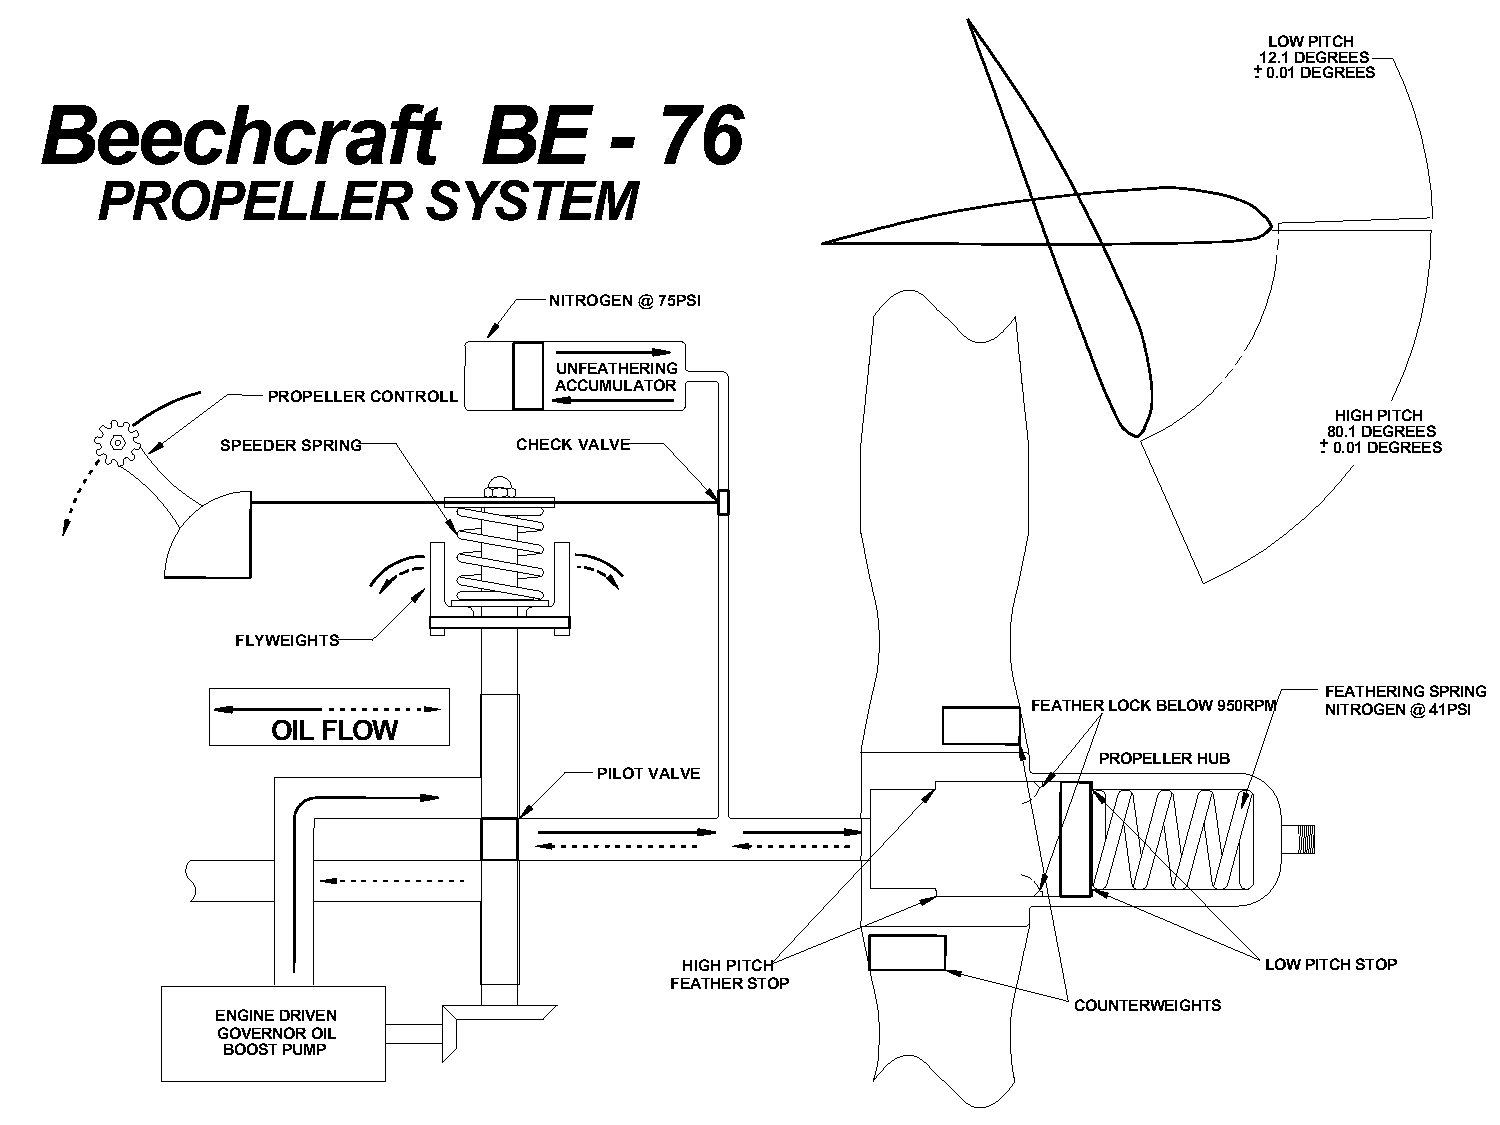
\includegraphics[width=1.0\linewidth]{be76-propeller}
\end{center}
\end{figure}

\newpage

\subsection{Landing Gear}

\begin{figure}[H]
\begin{center}
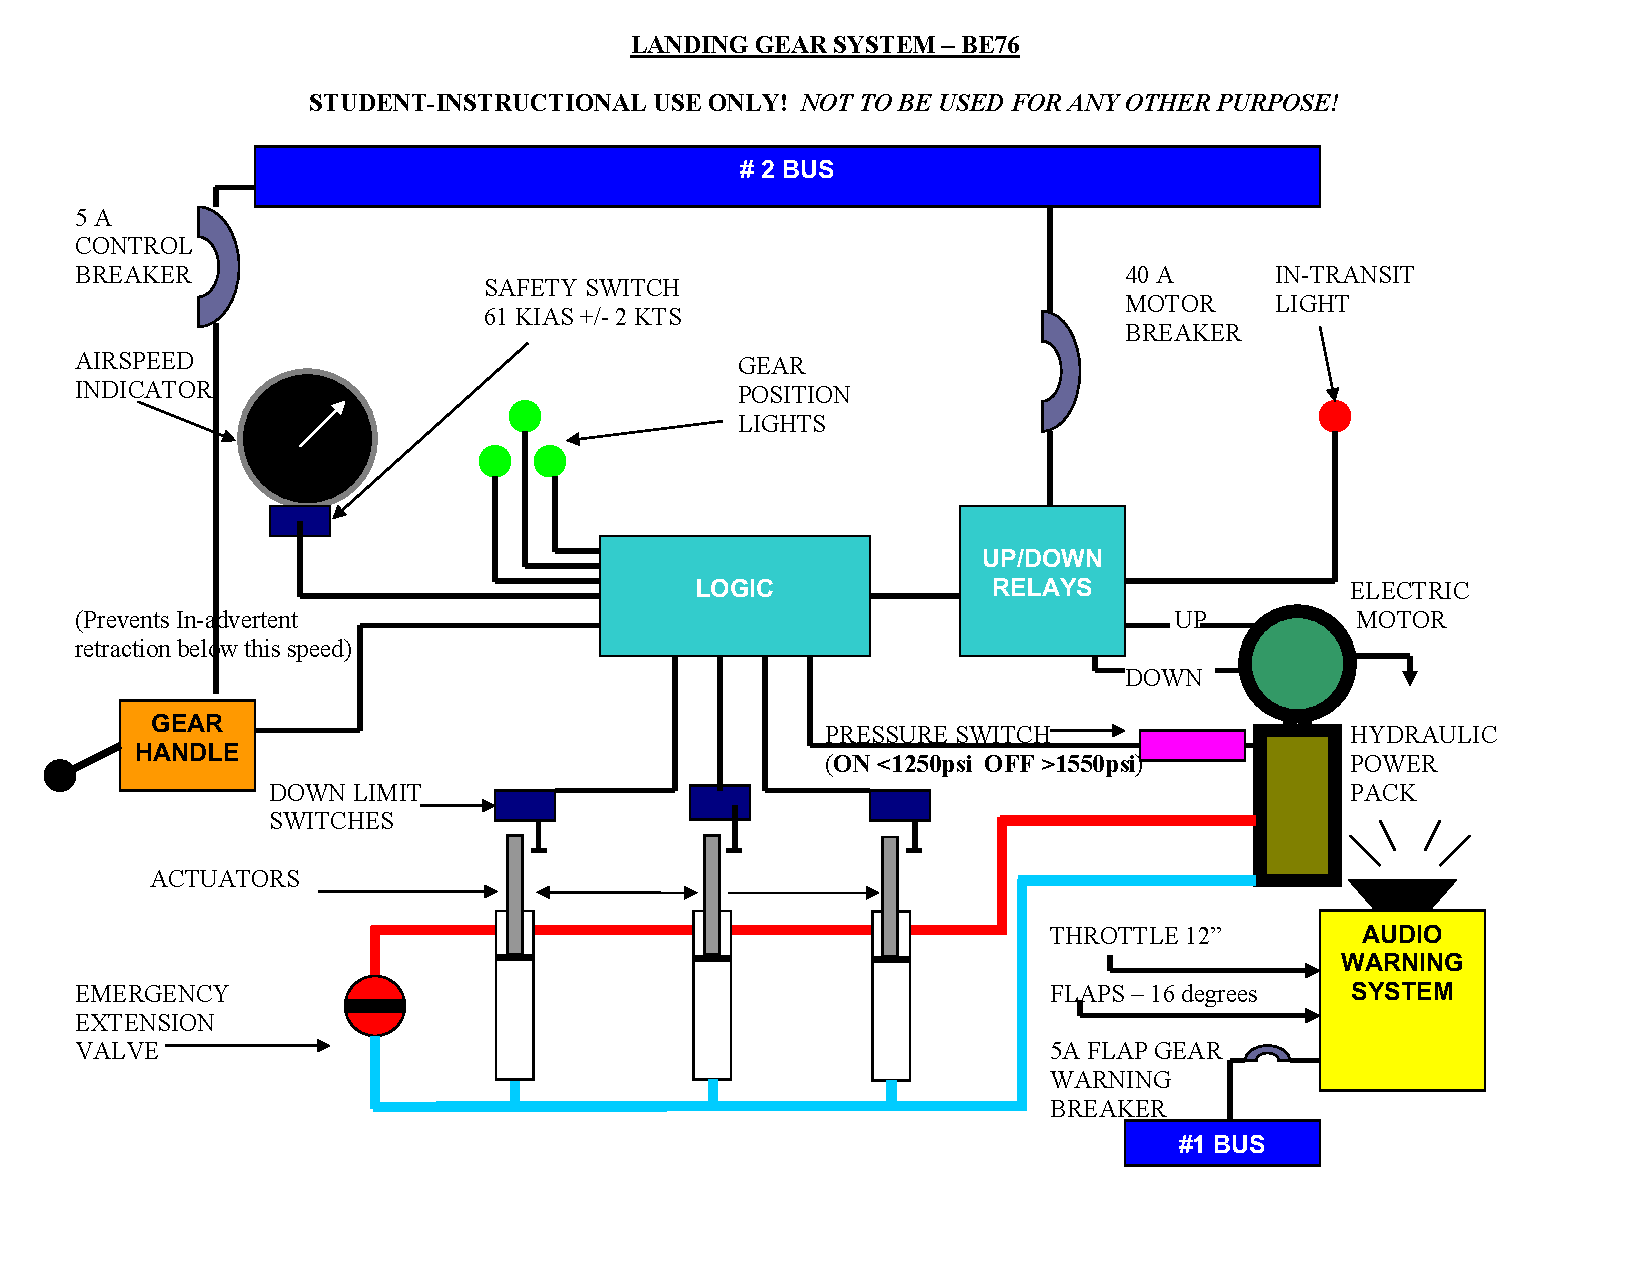
\includegraphics[width=1.0\linewidth]{be76-landinggear}
\end{center}
\end{figure}

\newpage

\subsection{Pressure System}

\begin{figure}[H]
\begin{center}
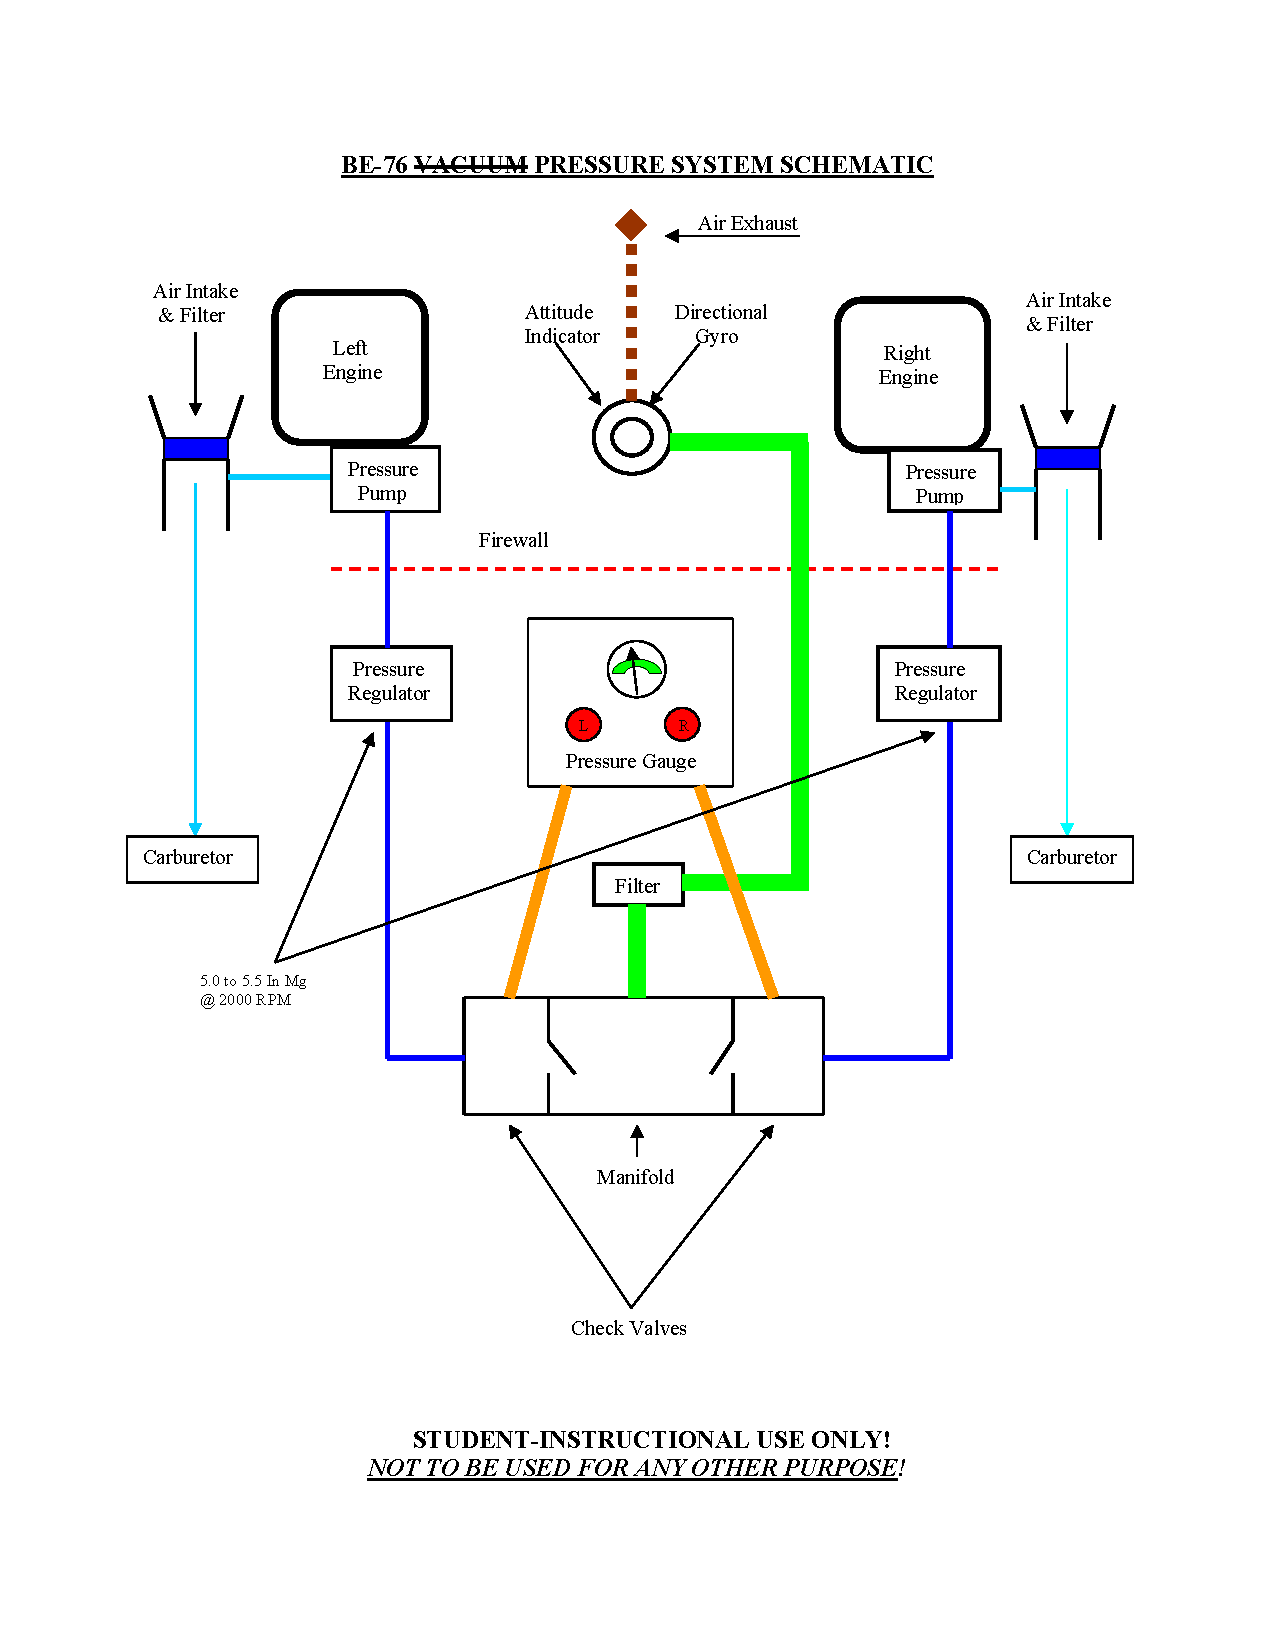
\includegraphics[width=1.0\linewidth]{be76-pressure}
\end{center}
\end{figure}

\newpage

\subsection{Fuel System}

\begin{figure}[H]
\begin{center}
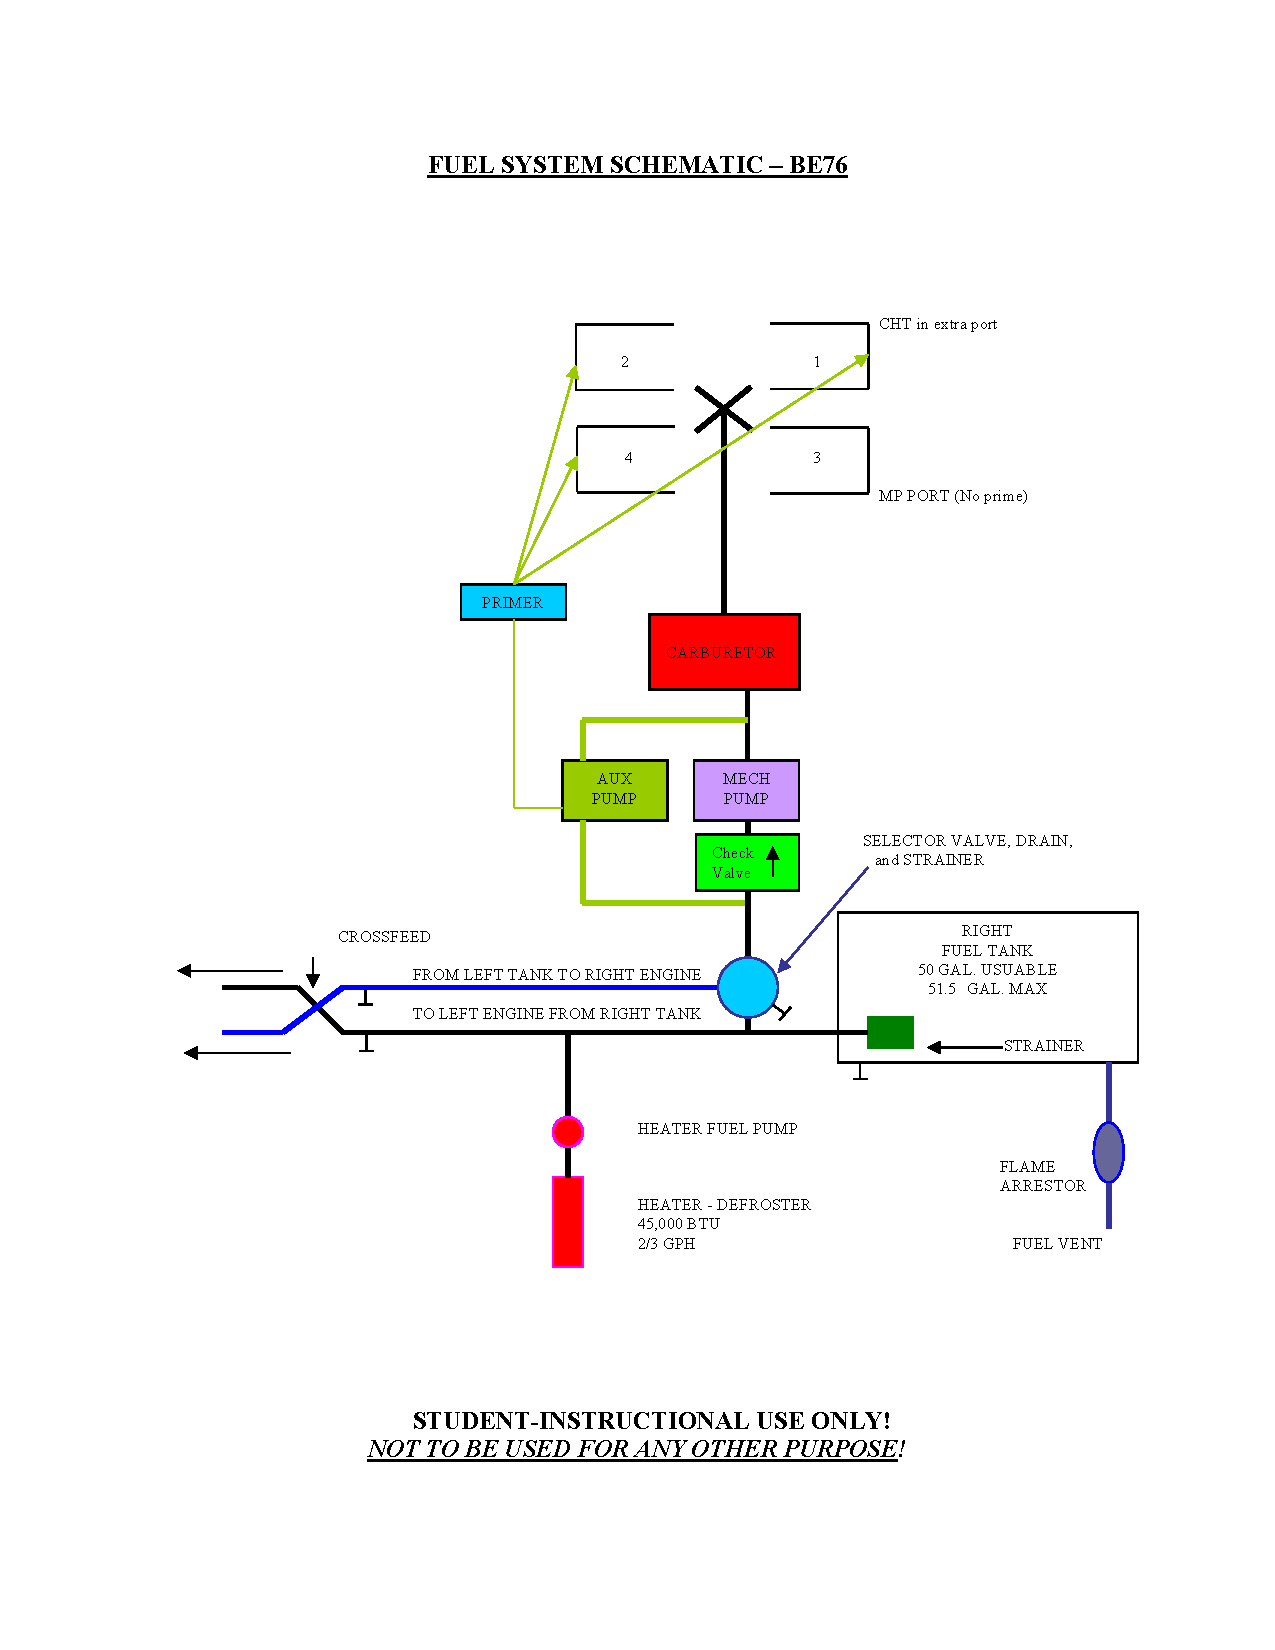
\includegraphics[width=1.0\linewidth]{be76-fuel}
\end{center}
\end{figure}

\newpage

\subsection{Electrical System}

\begin{figure}[H]
\begin{center}
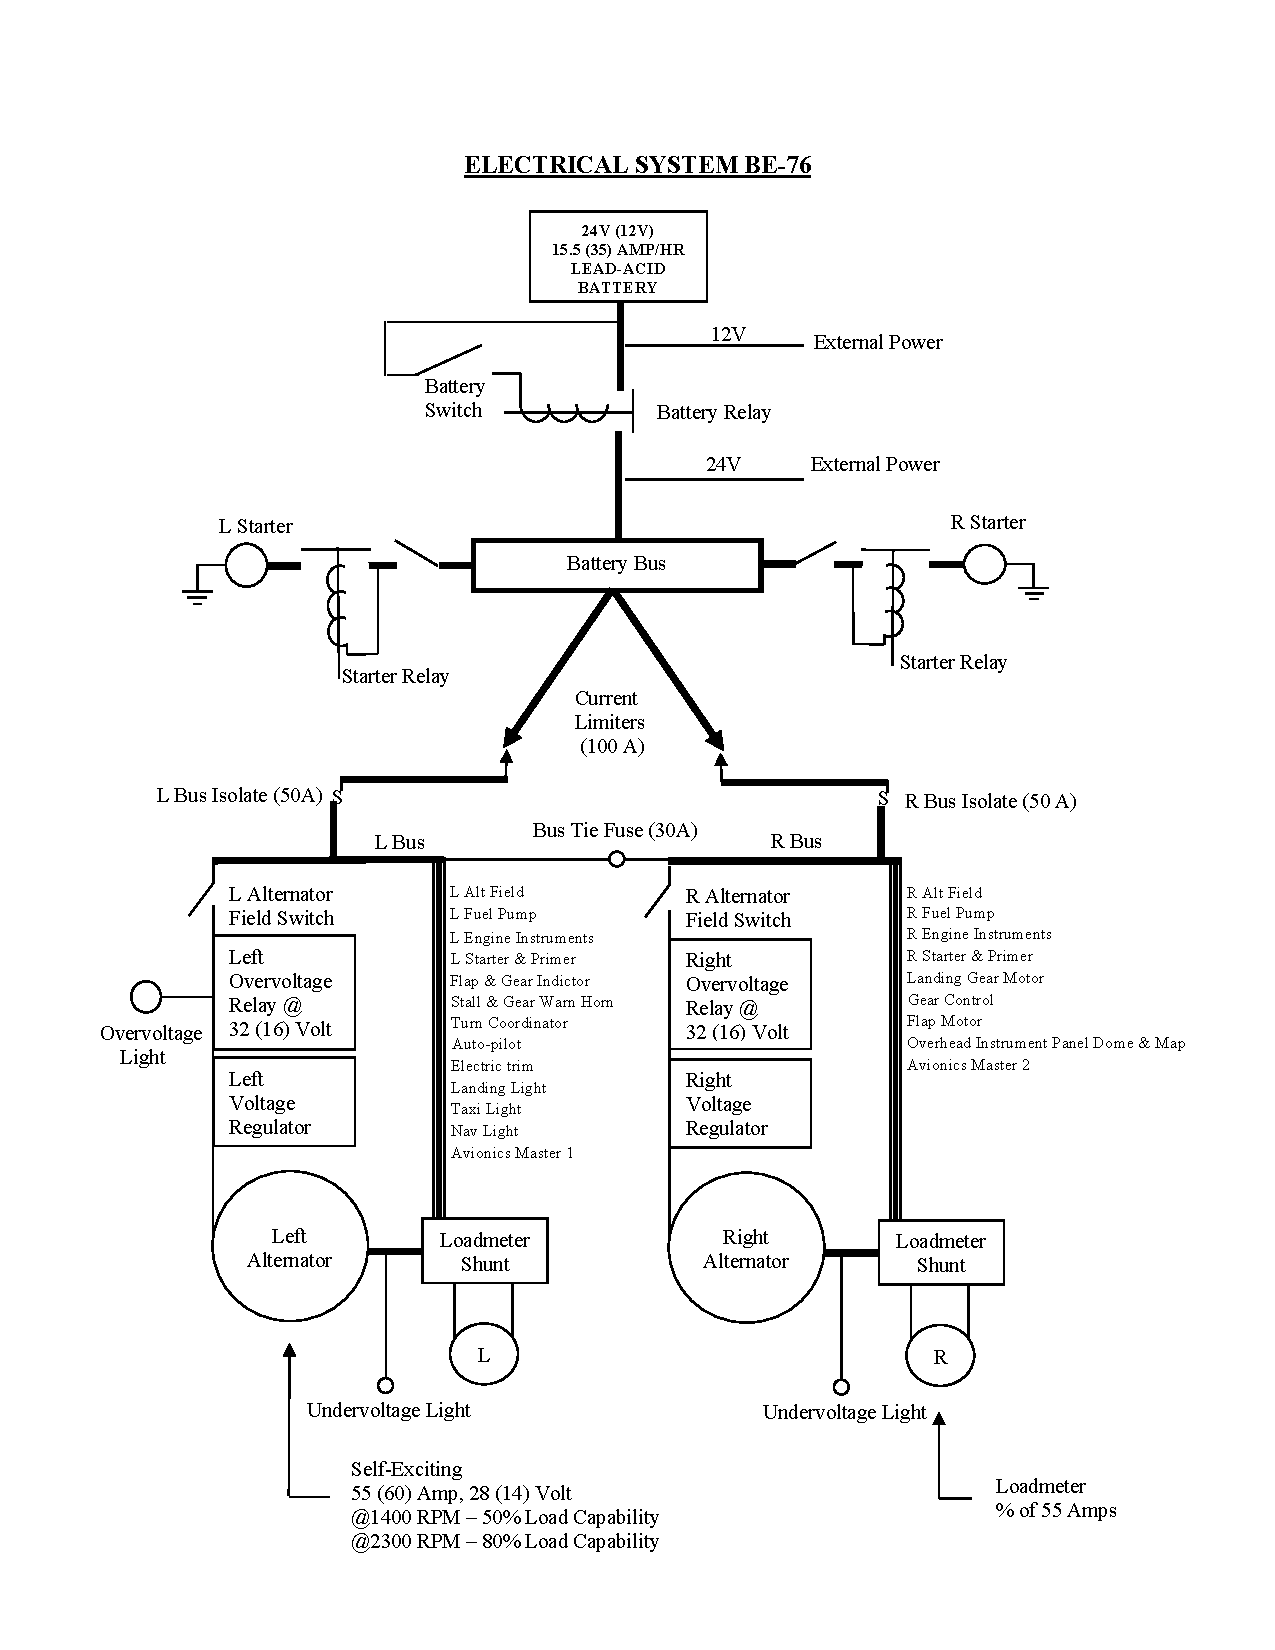
\includegraphics[width=1.0\linewidth]{be76-electrical}
\end{center}
\end{figure}

\chapter{Maneuvers}

\section{Introduction to Maneuvers}

All maneuvers begin and end the same way. Begin by clearing the area, followed by a power change (if required),
and a GUMP-CS check. The maneuvers end by re-establishing slow cruise (20''/2400), and doing a final GUMP-CS
check for cruise configuration.

\begin{table}[H]
\centering
\begin{tabular}{|c|l|c|c|}
\hline
                    &                                                 & \textbf{Maneuver Entry} & \textbf{Resume Cruise} \\ \hline
                    & \textcolor{blue}{\textbf{Power}}                & As Required             & 20'' MP                \\ \hline
\textcolor{blue}{G} & \textcolor{blue}{\textbf{G}}as (fuel selectors) & On                      & On                     \\
                    & \textcolor{blue}{\textbf{G}}as (boost pumps)    & On                      & Off                    \\ \hline
\textcolor{blue}{U} & \textcolor{blue}{\textbf{U}}ndercarriage        & As Required             & Up                     \\ \hline
\textcolor{blue}{M} & \textcolor{blue}{\textbf{M}}ixtures             & Rich                    & Cruise Lean            \\ \hline
\textcolor{blue}{P} & \textcolor{blue}{\textbf{Propellers}}           & As Required             & 2400 RPM               \\ \hline
\textcolor{blue}{C} & \textcolor{blue}{\textbf{C}}owl Flaps           & As Required             & Closed                 \\ \hline
\textcolor{blue}{S} & \textcolor{blue}{\textbf{S}}eat Belts           & Secure                  & Secure                 \\ \hline
\end{tabular}
\end{table}

Airman Certification Standards tables in this chapter are taken from from FAA-S-ACS-7B, Commercial Pilot for Airplane Category Airman Certification Standards, November 2023, and  FAA-S-ACS-25, Flight Instructor for Airplane Category, Airman Certification Standards, November 2023 as appropriate. Private pilot multi engine checkrides are rare, and maneuvers performed to the commercial standard are more than satisfactory for the private checkride's more forgiving tolerances.

\newpage

\section{Slow Flight}
\subsection{Maneuver Checklist}

\textbf{Perform clearing turns prior to maneuver. At least 3000' AGL.}

\begin{table}[H]
\centering
\begin{tabular}{|c|l|c|c|}
\hline
                    &                                                 & \textbf{Maneuver Entry} & \textbf{Resume Cruise} \\ \hline
                    & \textcolor{blue}{\textbf{Power}}                & \textbf{15'' MP}        & 20'' MP                \\ \hline
\textcolor{blue}{G} & \textcolor{blue}{\textbf{G}}as (fuel selectors) & On                      & On                     \\
                    & \textcolor{blue}{\textbf{G}}as (boost pumps)    & On                      & Off                    \\ \hline
\textcolor{blue}{U} & \textcolor{blue}{\textbf{U}}ndercarriage        & Down below 140 KIAS     & Up                     \\ \hline
\textcolor{blue}{M} & \textcolor{blue}{\textbf{M}}ixtures             & Rich                    & Cruise Lean            \\ \hline
\textcolor{blue}{P} & \textcolor{blue}{\textbf{Propellers}}           & 2400 RPM                & 2400 RPM               \\ \hline
\textcolor{blue}{C} & \textcolor{blue}{\textbf{C}}owl Flaps           & Open                    & Closed                 \\ \hline
\textcolor{blue}{S} & \textcolor{blue}{\textbf{S}}eat Belts           & Secure                  & Secure                 \\ \hline
\end{tabular}
\end{table}

Extend \underline{full flaps} when in the white arc of the airspeed indicator.

Maintain heading, altitude and an airspeed leading to the onset of the stall (stall horn intermittent, about 70 kts).
Pitch controls airspeed (use trim, up to full back!) and power controls altitude (approximately \underline{\textbf{15''-16''}}).

Recovery:
\begin{itemize}[label={}]
\item \textbf{23''} Power
\item Flaps up above \textbf{71 KIAS}
\item Gear up above \textbf{85 KIAS}
\item Perform post-maneuver GUMP-CS
\end{itemize}


\subsection{Airman Certification Standards}
\newpage

\section{Power-Off Stall}
\subsection{Maneuver Checklist}

\textbf{Perform clearing turns prior to maneuver. At least 3000' AGL.}

\begin{table}[H]
\centering
\begin{tabular}{|c|l|c|c|}
\hline
                    &                                                 & \textbf{Maneuver Entry} & \textbf{Resume Cruise} \\ \hline
                    & \textcolor{blue}{\textbf{Power}}                & \textbf{15'' MP}        & 20'' MP                \\ \hline
\textcolor{blue}{G} & \textcolor{blue}{\textbf{G}}as (fuel selectors) & On                      & On                     \\
                    & \textcolor{blue}{\textbf{G}}as (boost pumps)    & On                      & Off                    \\ \hline
\textcolor{blue}{U} & \textcolor{blue}{\textbf{U}}ndercarriage        & Down below 140 KIAS     & Up                     \\ \hline
\textcolor{blue}{M} & \textcolor{blue}{\textbf{M}}ixtures             & Rich                    & Cruise Lean            \\ \hline
\textcolor{blue}{P} & \textcolor{blue}{\textbf{Propellers}}           & Full forward below 90 KIAS & 2400 RPM            \\ \hline
\textcolor{blue}{C} & \textcolor{blue}{\textbf{C}}owl Flaps           & Open                    & Closed                 \\ \hline
\textcolor{blue}{S} & \textcolor{blue}{\textbf{S}}eat Belts           & Secure                  & Secure                 \\ \hline
\end{tabular}
\end{table}

Extend \textbf{full flaps} when in the white arc of the airspeed indicator.

Establish landing descent attitude: about 500 FPM @ 85 KIAS.

Pitch to maintain altitude and heading until stall warning or buffet: horizon to the glare shield.

Recovery:
\begin{itemize}[label={}]
\item \textbf{Full Power}, at least 65 KIAS (pitch for straight and level flight: VSI = 0)
\item Flaps up above \textbf{71 KIAS}
\item Gear up above \textbf{85 KIAS}
\item Perform post-maneuver GUMP-CS
\end{itemize}

\subsection{Airman Certification Standards}
\newpage

\section{Power-On Stall}
\subsection{Maneuver Checklist}
\subsection{Airman Certification Standards}
\newpage

\section{Steep Turns}
\subsection{Maneuver Checklist}
\subsection{Airman Certification Standards}
\newpage

\section{Accelerated Stall}
\subsection{Maneuver Checklist}
\subsection{Airman Certification Standards}
\newpage

\section{Emergency Descent}
\subsection{Maneuver Checklist}
\subsection{Airman Certification Standards}
\newpage

\section{Loss of Directional Control Demonstration (\vmc Demo)}
\subsection{Maneuver Checklist}
\subsection{Airman Certification Standards}
\newpage

\section{Effects of Configuration Demonstration (Drag Demo)}
\subsection{Maneuver Checklist}
\subsection{Airman Certification Standards}
\newpage







\chapter{Alphabet Soup}

This chapter contains a number of useful memory items for us to know.

\section{Required Equipment - VFR Day/Night}

A TOMATO FLAMES + FLAPS from 14 CFR 91.205.

\begin{itemize}
\item A - Altimeter
\item T - Tachometer
\item O - Oil Pressure Gage
\item M - Magnetic Compass
\item A - Airspeed Indicator
\item T - Temperature Gauge
\item O - Oil Temperature
\item F - Fuel Gauge
\item L - Landing Gear Position Indication
\item A - Anti Collision Lights (after a certain date?)
\item M - Manifold Pressure Gauge
\item E - Emergency Locator Transmitter (ELT)
\item S - Seat Belts
\item F - Floatation Equipment (Commercial)
\item F - Fuses
\item L - Landing Lights
\item A - Anti Collision Lights (after a certain date?)
\item P - Position Lights
\item S - Source of electrical power
\end{itemize}

\section{Required Equipment - IFR}

GRAB CARD + required equipment for VFR day and night.

\begin{itemize}
\item G - Generators or Alternators
\item R - Radio
\item A - Altimeter
\item B - Ball (Turn Coordinator)
\item C - Clock
\item A - Attitude Indicator
\item R - Rate of Turn
\item D - Directional Gyro
\end{itemize}

\section{Airworthiness - Required Paperwork}

ARROW

\section{Airworthiness - Required Inspections}

AVIATES

\begin{itemize}
\item A - Airworthiness Directives
\item V - VOR Check (30 days)
\item I - Inspections (100 hour, annual)
\item A - Altimeter
\item T - Transponder
\item E - ELT
\item S - Static System
\end{itemize}

\section{Landing Checklist}

GUMPS + FS or GUMPFSS

\begin{itemize}
\item G - Gas or fuel selector
\item U - Undercarriage
\item M - Mixture
\item P - Propeller
\item F - Flaps
\item S - Seat belts and harnesses
\item S - Switches: fuel pump, landing light, etc.
\end{itemize}

\section{Lost Communications Procedure - IFR}

AVE F MEA or ``Avenue F M.E.A.''.

\section{Aircraft Registrations}

30 FT DUC or ``thirty foot duck''.

\section{Special Use Airspaces}

MC PRAWN

\section{Kinds of Class E Airspace}

???

\section{Aeronautical Decision Making}

There are a whole bunch of these, let's group them together...





\printbibliography

\end{document}
